

\documentclass[12pt,a4paper]{book}

\usepackage[margin=8mm]{geometry}
\PassOptionsToPackage{defaults=hu-min,classmod=unchanged}{magyar.ldf}
\usepackage[magyar,english]{babel}
\usepackage{tikz,pgfplots}

%\documentclass{article}
\usepackage[utf8]{inputenc}
\usepackage{t1enc}
\usepackage[T1,T2A]{fontenc}
\usepackage{graphicx}
\usepackage{multirow}
\usepackage{natbib}
\usepackage{graphicx}
\usepackage{fancyhdr}
\usepackage{mathptmx}
\usepackage{geometry}
\usepackage{ifthen}
\usepackage{enumitem}
\usepackage{float}
\usepackage{capt-of}
\usepackage[section]{placeins}
\usepackage{dblfnote}
\usepackage{nomencl}
\usepackage{amsmath}
\usepackage{pgfplots}
\usepackage{graphicx}
\usepackage{epstopdf}
\usepackage{epsfig}
\usepackage{hyperref}
\usepackage{tikz}
\usepackage{filecontents}
\usetikzlibrary{shapes,arrows,positioning,calc}
\usepackage{amssymb}
\usepackage{gensymb}
\usepackage{datatool, filecontents}
\usepackage{svg}
%\usepackage{luacode}
\usepackage{multirow}
\usepackage{listings}
\usepackage{lipsum}
\usepackage{pgfplotstable, booktabs}
\usepackage{datatool,fp}
\usepackage{color}
\usepackage{amsfonts}
\usepackage[colorinlistoftodos]{todonotes}
\usepackage{algorithm}
\usepackage{algpseudocode}
\usepackage{blindtext}
\usepackage{titlesec}
%\usepackage[svgnames]{xcolor}
%\usepackage{newtxtext,newtxmath}
%\usepackage{etoolbox}



\makeatletter
% \patchcmd{<cmd>}{<search>}{<replace>}{<success>}{<failure>}
\patchcmd{\@makechapterhead}{\huge}{\large}{}{}% for \chapter
\patchcmd{\@makechapterhead}{\Huge}{\large}{}{}% for \chapter
\patchcmd{\@makeschapterhead}{\Huge}{\large}{}{}% for \chapter*
\makeatother


%----------------------------XML stilus
\definecolor{gray}{rgb}{0.4,0.4,0.4}
\definecolor{darkblue}{rgb}{0.0,0.0,0.6}
\definecolor{cyan}{rgb}{0.0,0.6,0.6}

\lstset{
  basicstyle=\ttfamily,
  columns=fullflexible,
  showstringspaces=false,
  commentstyle=\color{gray}\upshape
}

\lstdefinelanguage{XML}
{
  morestring=[b]",
  morestring=[s]{>}{<},
  morecomment=[s]{<?}{?>},
  stringstyle=\color{black},
  identifierstyle=\color{darkblue},
  keywordstyle=\color{cyan},
  morekeywords={xmlns,version,type}% list your attributes here
}

% From egreg at https://tex.stackexchange.com/questions/335483/retrieving-substring-of-dtlfetch
\newcommand{\DTLfetchsave}[5]{%
  \edtlgetrowforvalue{#2}{\dtlcolumnindex{#2}{#3}}{#4}%
  \dtlgetentryfromcurrentrow{\dtlcurrentvalue}{\dtlcolumnindex{#2}{#5}}%
  \let#1\dtlcurrentvalue
}


\usetikzlibrary{pgfplots.groupplots, matrix}
\usepgfplotslibrary{groupplots}
\pgfplotsset{%
    compat=1.12,
    minor grid style={dashed,red},
    major grid style={dotted,green!50!black},
    select coords between index/.style 2 args={
    x filter/.code={
        \ifnum\coordindex<#1\def\pgfmathresult{}\fi
        \ifnum\coordindex>#2\def\pgfmathresult{}\fi
    }
}}
\usepackage{subfig}
\captionsetup[subfigure]{labelfont={it,bf},textfont={it,bf},labelformat=parens,labelsep=space}
\usepackage{siunitx}
\usepackage{listings}



\tikzset{
block/.style = {draw, fill=white, rectangle, minimum height=3em, minimum width=3em},
tmp/.style  = {coordinate}, 
sum/.style= {draw, fill=white, circle, node distance=1cm},
input/.style = {coordinate},
output/.style= {coordinate},
pinstyle/.style = {pin edge={to-,thin,black}
}}

\newenvironment{kep}
{   \begin{center}

    \end{center}
}



\title{Kűltéri mobilis robot}								
\author{Gábor Szabolcs László}							
\date{20 Nov 2018}	

\makeatletter
\let\thetitle\@title
\let\theauthor\@author
\let\thedate\@date
\makeatother

\pagestyle{fancy}
\fancyhf{}
%\rhead{Share\LaTeX}
%\lhead{Guides and tutorials}
\rfoot{\center \thepage}

 \geometry{
 a4paper,
 total={170mm,257mm},
 left=25mm,
 right=25mm,
 top=20mm,
 bottom=25mm,
 headheight=15mm
 }
 
%%Formating figure cross references 
\makeatletter
\renewcommand\p@figure{ábra \thesection.\arabic{figure}\expandafter\@gobble}
\makeatother
 
\def\mand#1#2{#1#2} % "macro and"
 
\newcommand\xname{*}
\newcommand\x{*}
\newcommand\y{*}
\newcommand\z{*}
\newcommand\img{*}
\newcommand\imgSecond{*}
\newcommand\sources{*}
\newcommand\captionn{*}
\newcommand\watherProf{*}
\newcommand\sebesseg{*}
\newcommand\weight{*}
\newcommand\AcAndGy{*}
\newcommand\GPS{*}
\newcommand\figlabel{*}
\newcommand{\figlabela}{*}
\newcommand{\figlabelb}{*}
\newcommand{\figlabelc}{*}
\newcommand\svg{*}
\newcommand{\idoFelirat}{*}
\newcommand{\AbraFelirat}{*}
\newcommand{\GlobalPath}{*}
\newcommand{\GlobalPathA}{*}
\newcommand{\GlobalPathB}{*}
\newcommand{\GlobalPathC}{*}
\newcommand{\secondImage}{*}
\newcommand{\nth}{1}
\newcommand{\palya}{*}
\newcommand{\palyaA}{*}
\newcommand{\palyaB}{*}
\newcommand{\palyaC}{*}

\newcommand{\coefA}{1}
\newcommand{\coefB}{1}
\newcommand{\coefC}{1}

\newcommand{\aspectratioPic}{1}
\newcommand{\rotationAnglePic}{0}
\newcommand{\plotRotSpeed}{true}
\newcommand{\plotSpeed}{true}
%%\setfootsepline{.8pt}

% Egyqnlet referencia stilus.
\newcommand*{\myeqref}[2][egyenlet~]{%
  \hyperref[{#2}]{#1(\ref*{#2})}%
}
\def\equationautorefname#1#2\null{%
  Eq.#1(#2\null)%
}

% Egyqnlet referencia stilus intervalum.
\newcommand*{\myeqrefinterval}[3][egyenletek~]{%
  \hyperref[{#2}]{#1(\ref*{#2})-(\ref*{#3})}%
}


\DFNalwaysdouble % Double colon footnotes.

%\makenomenclature
%% This removes the main title:
\renewcommand{\nomname}{}
%% this modifies item separation:
\setlength{\nomitemsep}{8pt}
%% this part defines the groups:
%----------------------------------------------
\usepackage{etoolbox}
\renewcommand\nomgroup[1]{%
  \item[\bfseries
  \ifstrequal{#1}{R}{Rövidítsek}{%
  \ifstrequal{#1}{J}{Jelölősek}{
    \ifstrequal{#1}{B}{Number Sets}{%
    \ifstrequal{#1}{C}{Other Symbols}{}}
  }}%
  \ifstrequal{#1}{F}{Fizikai Konstansok}{%
    \ifstrequal{#1}{B}{Number Sets}{%
    \ifstrequal{#1}{C}{Other Symbols}{}
  }}%
]\vspace{8pt}} % this is to add vertical space between the groups.
%----------------------------------------------

% This will add the units
%----------------------------------------------
\newcommand{\nomunit}[1]{%
\renewcommand{\nomentryend}{\hspace*{\fill}#1}}
%----------------------------------------------

\nomenclature[R]{\textbf{ROS}}{Robot Operation System}
\nomenclature[R]{\textbf{DSC}}{Distributed Control System}
\nomenclature[R]{\textbf{GUID}}{Globally Unique Identifier -globálisan egyedi azonosító}
\nomenclature[R]{\textbf{SMC}}{Sliding Mode Control - Csuszas alapu szabalyzas}
\nomenclature[R]{\textbf{CTM}}{Computed Torque Method - Kiszamitott Nyomatekok modszere}
\nomenclature[R]{\textbf{VFO}}{Vector Field Orientation - Vektor alapu iranymeghatas}
\nomenclature[R]{\textbf{DDV}}{Diferential Driven Vehicles}
\nomenclature[R]{\textbf{ICR}}{Instantaneous Center of Rotation - pillanatnyi forgás-középpont}
\nomenclature[R]{\textbf{HLC}}{Hight Level Controller - magaszintu szabalyozo}
\nomenclature[R]{\textbf{OMP}}{Outdor Mobile Robot - kulteri mobilis robot}
\nomenclature[R]{\textbf{IMO}}{in my opinion}
\nomenclature[R]{\textbf{OP}}{original poster}
\nomenclature[R]{\textbf{COM}}{Center Of Mass}
\nomenclature[R]{\textbf{COG}}{Center Of Geometry}
\nomenclature[R]{\textbf{MR}}{Mobilis Robot }
\nomenclature[R]{\textbf{AMR}}{Autonomus Mobilis Robot }
\nomenclature[R]{\textbf{VNR}}{Vonatkoztatási Rendszer }
\nomenclature[R]{\textbf{UART}}{két vezetékes(Tx,Rx) két irányú kommunikáció}
\nomenclature[R]{\textbf{HLC}}{Angol elnevezésből származó rövidítése a Magasszintű szabályzónak (High Level Controller}

\nomenclature[R]{\textbf{URDF}}{Unified Robot Description Format, xml alapú robotleiró nyelv}

\nomenclature[R]{\textbf{AMCL}}{Adaptive Monte Carlo Localization}

\nomenclature[R]{\textbf{LIDAR}}{Light Detection and Ranging, 2D vagy 3D lézeres kép alkotó műszer}

\nomenclature[R]{\textbf{IMU}}{Inertial Measurement Unit gravitációs gyorsulást és szög elfordulást mérő szenzor.}

\nomenclature[R]{\textbf{SSMR}}{Skid-Steered Mobile Robot - csúszókormányzású mobilis robot.}

\nomenclature[R]{\textbf{4W-SSMR}}{4Wheel Skid-Steered Mobile Robot - 4 kerekű csúszókormányzású mobilis robot.}



\nomenclature[J]{$k$}{$k$ $\in(F, B) $ ahol F és B a robot első és hátulsó oldali kerekek jeleni. }
\nomenclature[J]{$i$}{$i$ $\in(L, R) $ ahol L és R a robot bal és jobb oldali kerekek jeleni. }
\nomenclature[J]{$n$}{$n$ $\in(G, R) $ ahol G és R világ és robot vonatkoztatási rendszer. }
\nomenclature[J]{$^n\S_i_k$}{Valemilyen $\S$ fizikai menyiseg a $n$ vonatkoztatási rendszerben,az $in$ indexek a mennyiség helyet jelöli.}
\nomenclature[J]{$h$}{Plank constant}
\nomenclature[J]{$X$}{A robot x tengelyen mert pozicioja\nomunit{$\, m$}}
\nomenclature[J]{$Y$}{A robot y tengelyen mert pozicioja\nomunit{$\, m$}}
\nomenclature[J]{$\theta$}{A robot z tengelyen x tengelyel bezart szoge\nomunit{$\, rad$}}
\nomenclature[J]{$F$}{erők\nomunit{$\, N$}}
\nomenclature[J]{$q_2$}{A $MR$ állapot vektora $q \in \mathbb{R}^3$ $q$ = [X Y $\theta$] ahol a X es Y  a robot x iletve y tengelyen mert pozicja}

\nomenclature[J]{\includesvg[width = 30pt]{SajatRobot/SzerkAbrak/IRQSymbol.svg}}{Megszakitas a proceszornak.}
\nomenclature[J]{\includesvg[width = 30pt]{SajatRobot/SzerkAbrak/AISymbol.svg}}{Analog bemenet.}
\nomenclature[J]{\includesvg[width = 30pt]{SajatRobot/SzerkAbrak/DISymbol.svg}}{Digitalis bemenet.}
\nomenclature[J]{\includesvg[width = 30pt]{SajatRobot/SzerkAbrak/DOSymbol.svg}}{Digitalis kimenet.}
\nomenclature[J]{\includesvg[width = 30pt]{SajatRobot/SzerkAbrak/uBSymbol.svg}}{Micriblaze proceszor cimtartomanyaban levo regiszter.}
\nomenclature[J]{\includesvg[width = 30pt]{SajatRobot/SzerkAbrak/DmuxSymbol.svg}}{Digitalis tobbites multiplexer.}
\nomenclature[J]{\includesvg[width = 30pt]{SajatRobot/SzerkAbrak/SmuxSymbol.svg}}{Multiplexert szelektalo regiszter.}

\nomenclature[F, 02]{$c$}{Speed of light in a vacuum inertial system 
\nomunit{$299,792,458\, m/s$}}
\nomenclature[F, 03]{$h$}{Plank Constant
\nomunit{$6.62607 \times 10^{-34}\, Js$}}
\nomenclature[F, 01]{$g$}{Gravitational Constant 
\nomunit{$6.67384 \times 10^{-11}\, N \cdot m^2/kg^2$}}
\pgfplotsset{compat=1.12}
\usepgfplotslibrary{external} % creates a tight self-contained pdf figure for each tikzpicture
\tikzexternalize % comment out to debug if latex errors: generates the external pdf
\tikzset{external/force remake} % otherwise will use external pdf if it exists
\tikzset{png export/.style={
	external/system call={
		pdflatex \tikzexternalcheckshellescape
			-halt-on-error -interaction=batchmode -jobname "\image" "\texsource";
		convert -units pixelsperinch -density 150 "\image.pdf" "\image.png";
		convert -units pixelsperinch -density 600 "\image.pdf" "\image-600.png";
}}}
\tikzset{png export}
\tikzsetexternalprefix{tikz/} % output the pdf to an existing directory (needs to exist)



\begin{document}

\renewcommand{\idoFelirat}{$Id$\H{o}$(s)$}

%\tracingall

%\begin{titlepage}
	

	\centering
    \vspace*{4 cm}
    
\includegraphics[scale=0.65]{Fedolap/SapientiaLogo1.png}\\
    [1.0 cm]	% 
   % \textsc{\LARGE  Sapientia \newline Erdélyi Magyar Tudomanyegyetem}\\[2.0 cm]	

	\rule{\linewidth}{0.2 mm} \\[0.4 cm]
	\centering
	{ \huge \bfseries \thetitle}\\
	\rule{\linewidth}{0.2 mm} \\[1.5 cm]
	
	\vspace*{4 cm}
	
	\begin{minipage}{0.4\textwidth}
		\begin{flushleft} \large
			\emph{Témavezető tanár:}\\
			Brassai Sándor Tihamér\\
			\end{flushleft}
			\end{minipage}~
			\begin{minipage}{0.4\textwidth}
            
			\begin{flushright} \large
			\emph{Diák :} \\
			Gábor Szabolcs László\\
		\end{flushright}
        
	\end{minipage}\\[2 cm]
\end{titlepage}
	\newpage

%\begin{titlepage}
Model tip a.



Declaraţie


Subsemnata/ul ............................................................., absolvent(ă) al/a specializării …………………………………………………………., promoţia………… cunoscând prevederile Legii Educaţiei Naţionale 1/2011 şi a Codului de etică şi deontologie profesională a Universităţii Sapientia cu privire la furt intelectual declar pe propria răspundere că prezenta lucrare de disertație se bazează pe activitatea personală, cercetarea/proiectarea este efectuată de mine, informaţiile şi datele preluate din literatura de specialitate sunt citate în mod corespunzător. 







Localitatea, 
Data: 							                  Absolvent
								Semnătura………………………
                                
                                
\newpage                                

\textbf{Model tip b.}


\textbf{Declaraţie }


Subsemnata/Subsemnatul .................................................., funcţia…………………….,
titlul ştiinţific………………… declar pe propria răspundere că absolventa/absolventul …………………………………......……………… de la specializarea …………………………………………………................. a întocmit prezenta lucrare sub îndrumarea mea.
Forma finală a lucrării a fost verificată de mine şi aceasta corespunde cerinţelor de formă şi conţinut precizate în Metodologia proprie de organizare a examenului de finalizare a studiilor (examen de licenţă/diplomă şi disertaţie) în cadrul Universităţii Sapientia din Cluj-Napoca. Lucrarea/proiectul corespunde şi cerinţelor impuse de Legea Educaţiei Naţionale 1/2011 cu modificări ulterioare, Codului de etică şi deontologie profesională a Universităţii Sapientia referitoare la furt intelectual.
Sunt de acord cu susţinerea lucrării în faţa comisiei de examen de disertație.





Localitatea, 
Data:					    			  Semnătura îndrumătorului, 
		



\end{titlepage}

\begin{titlepage}


\section*{Extras}
Subiectul tezei este implementarea sarcinilor legate de robotul mobil, care pot fi aplicate în teren și măsurătorile cu sistemul real. Robotul este un robot mobil de tip SSMR cu patru roți, cele patru roți sunt deplasate cu ajutorul unui raport de transmisie mare, raportul de transmisie este 1:70, iar viteza maximă a roții este de 90 \degree / s, iar diametrul roților este de 0,40m.

Am folosit controale PID pentru a controla viteza de rotație a roților, pe care le-am implementat pe o pagină de dezvoltare bazată pe FPGA și pe software.

Cu ajutorul Matlab, am estimat funcția de transmisie a sistemului și apoi folosind-o informațiile primite am proiectat controlorii PID. La proiectarea sistemului, am analizat oportunitățile de cercetare și dezvoltare, astfel încât este posibilă integrarea altor tipuri de controlere hardware și software în sistem, cu efort minim.

Sarcini centrale ale sistemului sunt realizate de către un computer mic, care rulează în sistemul de operare Ubuntu Linux. Programele rulate pe computer au fost implementate în mediul ROS în C / C ++.

Cu ajutorul senzorilor incrementali, măsor viteza de rotație a roților. Curentul motoarelor DC, care  conduc rapoartele de transmisie, măsor cu senzori bazați pe efect hall.

Valorile măsurate procesez cu ajutorul lui FPGA și trimit mai departe la computerul central.

Unul dintre subiectele principale ale disertației a fost de a examina soluțiile posibile pentru integrarea FPGA și ROS.

Soluția ROS-serial, ca o posibilă soluție de integrare generală, oferită de ROS, este utilizată pe scară largă pentru a integra hardware-ul la nivel inferior, dar datorită limitărilor sale nu este capabil să gestioneze pachetele mari de mesaje.

Pe baza rezultatelor, opțiunea de comunicare cu cele mai bune performanțe este crearea unui protocol propriu bazat pe UART. Cu această soluție, sistemul funcționează robust cu o perioadă de eșantionare de 1 ms. În prezent, lungimea mesajului între calculatorul central și modulele FPGA poate fi de până la 200 de byte, care pot fi extinse dacă este necesar.

Modulele din FPGA au fost implementate folosind un Matlab / Generator de sistem, de ex. PWM, modul de comunicare UART.

Avantajele protocolului propriu dezvoltat și ale FPGA sunt că, prelucrarea datelor încorporate în FPGA este făcută de hardware, facilitând încărcarea procesorului. Dacă protocolul de comunicație a fost efectuat de către procesorul de bază uBlaze soft core, datorită numeroaselor întreruperi, sistemul a fost inutilizabil pentru eșantionarea la 20 ms.

Interpretul de instrucțiuni directe încorporat în modulul de comunicație FPGA poate opri ieșirea PWM și controlorii, dacă întrerupe comunicarea sau asta solicită unitatea centrală.

HeartBeat-ul, cu ajutorul unei soluție de securitate, monitorizează funcționarea tuturor nodurilor importante rulate în sistemul ROS, inclusiv funcționarea FPGA-urilor. Nodul HearBeat trimite periodic semnale de permisiune și așteaptă semnale de la module inportante.

Monitorizarea cadrului și interpretarea caracterelor speciale sunt realizate de hardware-ul FPGA, iar datele primite sunt scrise în memoria partajată cu procesorul. Dacă pachetul este pe deplin în memorie, atunci cere procesorului să-și întrerupă activitatea și să prelucrează pachetul.

Înclinarea și accelerațiile robotului sunt măsurate cu ajutorul unui modul IMU.

Cu ajutorul senzorului 2D LIDAR, măsor distanța robotului în raport cu obiectele din apropiere, distanța de până la 8m, precizia 360 grade, 2mm. Folosind măsurătorile LIDAR, cu ajutorul HectorSlam-ului fac o hartă a mediului, în care robotul este capabil să autolocalizeze.

LIDAR-ul este, în principiu, foarte potrivit pentru sarcini de cartografiere, dacă mediul conține pereți de sticlă și în apropiere nu poate fi găsit alt obiect stabil, în cartografiere apar zgomote.


\subsection*{ Măsurători cu robotul}

Măsurătorile cu robotul, au fost efectuate în diverse terene, studiind pe traseu circular și rotație pe loc. Pe măsură ce robotul se mișcă pe scări, rezultă că scara trebuie abordată mai eficient cu un centru de greutate și nu perpendiculară. Când se deplasează pe sol nisipos, viteza mică a roților este mai eficientă, deoarece roțile nu se sapă în nisip.



\subsection*{Controlul poziției}

Controlul  poziției la robot, poate fi împărțit în două sub-sarcini: întoarce la destinație și reduce distanța dintre ținta și poziția curentă. În cazul direcției, reglăm unghiul în timp ce în cazul distanței pe viteza. Pentru ambele cantități, am folosit un controler de tip PI, ponderând intrarea controlerului de distanță cu valoarea inversă al erorii controlerului de poziției unghiului.
\end{titlepage}
\begin{titlepage}

\section*{Kivonat}

A dolgozat témája terepen alkalmazható mobilis robothoz köthető feladatok elvégzése, és mérések a valós rendszerrel. A robot egy négykerekű csúszáskormányzású SSMR típusú mobilis robot, a négy kereket egy nagy fogaskerék áttétel segítségével hozzuk mozgásba, az áttétel aránya 1:70, és a kerék maximális forgási szögsebessége 90\degree/s, a kerekek átmérője 0.40m.
A kerekek forgási sebességének a szabályzására PID típusú szabályzókat alkalmaztam, amelyeket FPGA alapú fejlesztőlapon és szoftveresen valósítottam meg.
Matlab segítségével megbecsültem a rendszer átviteli függvényét és ezután felhasználva terveztem meg a PID szabályzókat. A rendszer tervezésénél figyeltünk a kutatás-fejlesztési lehetőségekre, így lehetőség van más típusú hardveres és szoftveres szabályzókat is integrálni a rendszerbe minimális erőfeszítéssel.

A rendszer központi feladatait egy kis méretű számítógép végzi, amelyen Ubuntu Linux alapú operációs rendszer fut. A számítógépen futó programokat ROS környezetben implementáltam C/C++ nyelven.

Inkrementális szenzorok segítségével mérem a kerekek forgási sebességét, hall effektusra alapuló szenzorokkal a fogaskerék áttételeket hajtó DC motorok áramát.

A mért értékeket FPGA segítségével dolgozom fel, és küldöm tovább a központi számítógépnek.

A dolgozat egyik fő témája az FPGA és ROS integrációjának lehetséges megoldásainak vizsgálata volt.
A ROS által nyújtott ROS-serial lehetséges általános integrációs megoldás széles körben alkalmazható alacsony szintű hardverek integrálására, de korlátai miatt nem képes nagy méretű üzenetcsomagok kezelésére.

Az eredmények alapján a legjobban működő kommunikációs lehetőség UART protokollra épülő saját protokoll készítése. Ezen megoldással a rendszer 1ms mintavételezési periódussal robusztusan működik. Jelen pillanatban az üzenet hossza a központi számítógép és az FPGA modulok között maximum 200 byte lehet, ami szükség esetén kiterjeszthető.
Az FPGA-ban levő modulokat Matlab/System Generator használatával valósítottam meg pl: PWM, UART kommunikációs modul.

A kifejlesztett saját protokoll és az FPGA előnyei, hogy az FPGA-ba beékező adatok feldolgozását a hardver végzi, így könnyítve a processzor leterheltségén. Abban az esetben, ha a kommunikációs protokollt a uBlaze soft core processzor végezt,e a sok megszakítás miatt a rendszer használhatatlan volt már 20ms mintavételezésnél.

Az FPGA kommunikációs modulba beépített direkt utasítás értelmező képes a PWM kimenetet és a szabályzókat leállítani abban az esetben, ha a kommunikáció megszakad vagy ha a központi egység ezt kéri.
A HeartBeat biztonsági megoldás segítségével figyeli a ROS rendszerben futó összes létfontóságú Node működését, beleértve a FPGA-k működését is. A HearBeat node periodikusan küld engedélyező jeleket és vár is a létfontóságú moduloktól.

A keret figyelését és a speciális karakterek értelmezését a FPGA  hardvere végzi, a beérkező adatokat a processzorral közös memóriába írja bele. Ha a csomag teljes egészében a memóriában van akkor, kéri a processzort, hogy szakítsa meg a munkáját és dolgozza fel a csomagot.






 A robot dőléseit és gyorsulásait IMU modul segéltségével mérem.

A 2D LIDAR szenzor segítségével mérem a robot távolságát a környezetében levő tárgyakhoz képest, 8m távolságig, 360\degree, 2mm pontossággal. A LIDAR méréseit felhasználva, HectorSlam segítségével térképet készítek a környezetéről, amelyben a robot képes lokalizálnia magát.
A LIDAR alapvetően jól használható a térképezési feladok elvezésére, abban az esetben, ha a környezet tartalmaz üvegfalat és nincs más stabilan mérhető tárgy a közelben, zajok jelennek meg a térképezésben. 

\subsection{Mérések a robottal}

A robottal méréseket végeztünk különböző terepviszonyok között, körpályán való mozgást és a helyben forgást tanulmányozva. A robot lépcsőn felfele való mozgását tanulmányozva az eredmény az, hogy a lépcsőt hatékonyabb súlyponttal előre, és nem merőlegesen kell megközelíteni. A homokos talajon való mozgás esetén a kerekek kis fordulatszáma hatékonyabb, mert így a kerekek nem ássák be magukat a homokba. 



\subsection{Pozíció szabályzása}

A  pozíció szabályzása a robotnak két részfeladatra osztható: fordulás a  cél irányába, és csökkentsd a távolságot a cél és az aktuális pozíció között. Az irány esetében szöget szabályzunk, míg a távolság esetében sebességet. Mindkét mennyiség esetében PI típusú szabályzót alkalmaztam, a távolság szabályzó bemenetét súlyozva a szögpozíció szabályzó hibájának a fordított értékével.






Kulcsszavak: SSMR,FPGA,ROS,Robot,SLAM

\end{titlepage}

\begin{titlepage}

\section*{Abstract}

The purpose the document is designing, implementing of a mobile robot platform, which can be applicable outdoor, like in agriculture, and measuring whit robot real scenarios. The robot is a four wheeled robot, the wheels was driven by a worm gearbox 1:70. Some parameters: radius of wheel 0.2m m, maximum angular speed of wheel 90 \degree/s. 
I used PID controllers to control the rotation speed of the wheels, which was implemented in the FPGA based soft core processor (uBlaze). 

With the help of Matlab, I estimated the transmission function of the system and then, with the help of this information I designed the PID controllers.
At the designing of the system, we paid attention to the development opportunities of the research, so it can be possible to integrate other types of hardware and software controllers into this system, with minimal effort.

The system's central tasks are performed by a small computer, running on Ubuntu Linux-based operating system. The running programs on the computer were implemented in ROS environment in C / C ++.

I measure the speed of rotation of the wheels with incremental sensors and the current of the DC motors, which drives the gear ratios, with sensors based on hall effect.I processed the measured values with the help of FPGA and send to the central computer.

One of the main topics of the dissertation was to examine possible solutions of FPGA and ROS integration.

The ROS-serial like a possible general integration, as a solution provided by ROS, is widely used to integrate low-level hardware, but due to its limitations, it is unable to handle large message packages.  Unable to use for integration FPGA and Ros, but successful applied for communication between IMU+ESP8266 (arguing based) and ROS use standard ROS messages.


Based on the results, the best-performing communication option, is to create own protocol, based on UART. With this solution, the system works robustly with 1ms sampling period. At the moment, the length of the message between the central computer and the FPGA modules can be up to 200 bytes, which can be extended if necessary.

The modules in the FPGA were implemented using a Matlab / System Generator, eg PWM, UART communication module. The advantages of the own developed protocol and FPGA, are that the processing of the data embedded in the FPGA is done by the hardware, making it easier for the processor to load.
If the communication protocol was performed by the uBlaze, the soft core processor due to many interruptions, the system was unusable from 20ms of sampling.


The direct instruction interpreter, built into the FPGA communication module, can stop the PWM output and the controllers, if the communication is interrupted or the central unit requests this.

The HeartBeat, uses the security solution to monitor the operation of all important Node running in the ROS system, including the operation of FPGAs. HearBeat node periodically sends permitting signals and waits for critical modules.

The monitoring of the frame and the interpretation of special characters are performed by the hardware of the FPGA, the incoming data is written to the common memory of the processor. If the package is fully in memory, then it asks the processor, to interrupt its work and process the package.

The inclinations and accelerations of the robot are measured with the help of an IMU module.

With the help of the 2D LIDAR sensor, I measure the distance of the robot in relation to the objects in around, up to 8m distance, 360 degree, with 2mm accuracy. Used the LIDAR Measurements, with the help of HectorSlam I create a map of its environment, in which the robot can locate itself.

LIDAR is basically well suited for mapping tasks, if the environment contains a glass wall and can’t find any other stable object in the area, noises appear in the mapping.



\subsection*{Measurements whit robots}

With the robot, we made some measurements in various surface conditions like: green grass, marble, pebbly surfaces to study the circular path motion, the rotation on place turning and robot motion on stair. Result of these measurements is the motion on stair is most effective when the center of gravity point is front and the angle between the stair and robot orientation is less than 90\degree. The motion of pebbly surface is most effective when the wheel rotation speed is smaller, because avoided the wheel sinking into sand.


\subsection*{Robot Position Controller}

The position controller of the robot can be divided by two sub task: turn to the destination and reduce the distance between the target and the current positionl. In the case of the direction we adjust the angle, while in case of distance the speed. For both quantities, I used a PI type controller, weighting the distance controller input with the inverse of the angle position controller error.

Keywords: SSMR,FPGA,ROS,Robot,SLAM

\end{titlepage}





\tableofcontents

\listoffigures

\listoftables\newpage

\printnomenclature[2cm] \newpage




\chapter{Bevezető}
A robotokat széles körben alkalmazzák, egyre több feladatra és most már az átlag emberek életében is. Néhány nagyobb vállat mint pl: ABB, Kuka nagy területet foglalt el az iparban robot karok gyártásában.Emellett egyre több kisebb vállalat jelent meg, amelyek háztartási vagy fél katonai eszközöket gyártanak pl.: iRobo. A mezőgazdaságban is próbálnak alkalmazni autonóm robotokat pl.: echorobotics amelyek segítségével hatóanyag mentes élelmiszereket állíthatnak elő.

A dolgozat célja hogy felderítse az aktuális legmodernebb technikákat amelyeket robotokon alkalmaznak, és ezeket alkalmazza egy kültéri mobilis robot megépítése során.
Az előzőleg már egy hasonló rendszer kivitelezésekor elteszitek modulok továbbfejlesztése és integrálása az új rendszerbe. A robot mozgása négy csiga áttétel és négy DC motor segítségével valósul meg. A motrok szögsebességét és  felvett arámokat merjük, inkrementális szenzor és elektromágneses jelenségre alapuló aramerő modul segítségével.

A beavatkozás feszültség formájában történik, amelyet H-híddal állítunk elő azáltal hogy PWM jelet generálunk.

Az inkrementális és aramerő szenzorok jeleit FPGA alapú fejlesztőlapokkal oldjuk meg. A roboton helyet foglal egy kis méretű számítógép is amely USB vezetékeken keresztül csatlakozik az FPGA lapokhoz és a roboton található más szenzorokhoz pl: LIDAR, IMU, GPS..
Az FPGA modulok segitsegevel valosulnak meg a kerekek szogsebesseg szabalyzasa, a dolgozatban targyalasra kerul az egyedi hardver integracioja ROS keretrendszerben, amelyet egy koztes nodal valositunk meg.
A robot a csiga áttelek miatt nagy nyomatékot tud előállítani, ami a mozgási sebesség rovására vált. A robot kepés 0.3 m/s sebességél mozogni előre, és 20 \degree/s forgási sebességet generálni súlypontja körül.

A dolgozat célja az elkészített kültéri mobilis robottal meréseket végezni különböző terepviszonyok között és azokat összehasonlítási. A terepviszonyok mit pl: füves, kavicsos, aszfalt, márvány stb. A meréseket szeretnek összehasonlítani a terepviszonyok függvényében: a robot mozgását és a szükséges energia nagyságát, a környezetében okozott behatások.

A robot SLAM algoritmus  dolgozza fel a LIDAR által mért adatokat és egy 2D térképet állít elő, amelyen kepés egyidőben behatárolnia pozícióját és a térképet építeni is. Ezen meglevő programok használatával kültéri meréseket végezni, térképeket készíteni és majd egy előírt pályán végigmenni, ezen terepeken a térképet használva. Az esetleges zavao tenyezok felderites amelyek befolyasoljak a terkepezes es a lokalizacio pontosagat.
\newpage
\FloatBarrier 



\chapter{Bibliográfiai tanulmány} 



\section{Robotok} 

Az olyan gépek, amelyeket arra terveztek, hogy bizonyos feladatokat automatikusan elvégezzenek gyorsabban és pontosabban mit az emberek. Manapság már sok típusú robot létezik, ezek közül néhány repül, földön gurul vagy mászik, de léteznek mar emberhez hasonlóak is. 



A robotok legelőször a második világháború alatt jelentek meg mint irányított bombák. A háború után W.Grey Walter neurologus fejlesztett ki egy kisméretű robotot (Elmer and Elsie) mely fényszenzorral, es nyomásszenzorral volt ellátva. 1961-1963 Johns Hopkins Beast robot képes volt a fal menten végigmenni és megtálalni a töltőállomást. 1970 -ben Shakey robot képes volt kamera segítségével egy vonalat követni. A 1990 után a fejlesztések felgyorsultak es azóta mar robot jár a naprendszer más bolygóján is. 



Ezen dolgozat csak a $MR$ típusú robotokkal fog részletesebben kitérni. A $MR$ típusú robotok képesek a saját pozíciójukat megváltoztatni a környezetükhöz képest. Az $AMR$ típusú robotok képesek saját környezetük felderítésére ismeretlen környezetben is különböző szenzorokat használva melyekkel kepések a környezetük paramétereinek a megmérésére. Az $AMR$ típusú robotokat manapság leginkább tároló helységekben használjak, ahol anyagokat, palettákat vagy különböző dolgokat kel egyik helyszínről a másikra szállítani (például Mobile Industrial Robots ApS vállalat fejlesztései). 



\section{Mobilis Robotok Helyváltoztatása} 

A $MR$ kerekekkel, hernyótalpakkal, vagy lábakkal képesek helyüket megváltoztatni. A leginkább használatos es robusztusnak bizonyult kültéri terepen a kerekek es a hernyótalpak. 

Legismertebb robot felépítések: packboot pl: iRobo510, 

négy hagyományos kerek pl: husky, négy kormányozható kerek, hat kerek, amiből négy kormányozható pl: Curiosity Mars Rover. 

Az utóbbi években a kerek fogalma is újraértelmeződőt, a hagyományos kerekek pl: RHex Rough-Terrain amely a kerek es a lábak keveréke. 





\section{Kültéri mobilis robotok} 





\renewcommand{\xname}{iRobo510}
\renewcommand{\x}{0.521}
\renewcommand{\y}{0.686}
\renewcommand{\z}{0.178}
\renewcommand{\weight}{20}
\renewcommand{\img}{MobilisRobotok/iRobo/iRobo510.jpg}
\renewcommand{\sources}{Forrás: https://www.army-technology.com}
\renewcommand{\captionn}{iRobo 510 lanctalpas packboot}
\renewcommand{\watherProf}{Igen -3m ig.}
\renewcommand{\sebesseg}{9.3}
\renewcommand{\weight}{10.89}
\renewcommand{\AcAndGy}{Igen}
\renewcommand{\GPS}{Igen}
\subsection*{iRobo510}
 A robot kulteren es belteren is egyarant hasznalhato, felderitesekre es kisebb beavatkozasra alkalmas a manipulatorat hasznalva.A robotot 2007 ben dobtak pacra. A katonasag hasznalta bombak hatastalanitasara vagy felderitesre. 

\renewcommand{\aspectratioPic}{0.5}
\begin{kep}
\begin{figure}[H]
\centering
\ifthenelse{\equal{\svg}{*}}
{
    \includegraphics[width=\aspectratioPic\textwidth,angle=\rotationAnglePic]{\img}
}
{
    \includesvg[width=\aspectratioPic\textwidth,angle=\rotationAnglePic]{\img}
}

 \ifthenelse{\equal{\sources}{*}}
    { \captionof{figure}{ \captionn}}
    { \captionof{figure}{ \mand{\mand{\captionn}{Forrás:}}{}} }
  	

\ifthenelse{\equal{\figlabel}{*}}
    {}
    {\label{fig:\figlabel}}%
    
\renewcommand{\figlabel}{*}



\end{figure}
\end{kep}
\renewcommand{\aspectratioPic}{1}
\renewcommand{\rotationAnglePic}{0}
\renewcommand{\svg}{*}


\begin{center}
\center
\begin{tabular}{ llll  }
 \hline
 Tulajdonság              &           &          & Mértékegység \\ \hline
\multirow{3}{*}{Méretek} & X         &    \x      & m  \\
                         & Y         &    \y      & m  \\
                         & Z         &    \z      & m  \\
Önsuly                   & \multicolumn{2}{l}{\weight} & kg \\
Max Sebesség             & \multicolumn{2}{l}{\sebesseg} & km/h \\
Gyorsulásmérő és Giroszkóp & \multicolumn{2}{l}{\AcAndGy} & 
\end{tabular}
\end{center}

 

\renewcommand{\xname}{Husky}
\renewcommand{\x}{0.99}
\renewcommand{\y}{0.67}
\renewcommand{\z}{0.39}
\renewcommand{\weight}{50 + 75}
\renewcommand{\img}{MobilisRobotok/clearpathrobotics/husky.jpg}
\renewcommand{\sources}{Forrás: https://robots.ros.org/husky}
\renewcommand{\captionn}{Négykerekű mobilis platform.}
\renewcommand{\watherProf}{Igen}
\renewcommand{\sebesseg}{3.6}
\renewcommand{\AcAndGy}{Igen}
\renewcommand{\GPS}{Igen}

\subsection*{Husky}
Nagy teherbírású kültéri mobilis robot, leginkább kutatási célokra használják, nagy keréknyomatéka miatt nehéz terepen is jól boldogul. Nagy felbontású inkrementális szenzorokkal szerelték fel, alacsony mozgási sebességre is képes. Működése 3 óra átlagos használat mellett, támogatja teljes mertekben ROS-t.

\renewcommand{\aspectratioPic}{0.6}
\begin{kep}
\begin{figure}[H]
\centering
\ifthenelse{\equal{\svg}{*}}
{
    \includegraphics[width=\aspectratioPic\textwidth,angle=\rotationAnglePic]{\img}
}
{
    \includesvg[width=\aspectratioPic\textwidth,angle=\rotationAnglePic]{\img}
}

 \ifthenelse{\equal{\sources}{*}}
    { \captionof{figure}{ \captionn}}
    { \captionof{figure}{ \mand{\mand{\captionn}{Forrás:}}{}} }
  	

\ifthenelse{\equal{\figlabel}{*}}
    {}
    {\label{fig:\figlabel}}%
    
\renewcommand{\figlabel}{*}



\end{figure}
\end{kep}
\renewcommand{\aspectratioPic}{1}
\renewcommand{\rotationAnglePic}{0}
\renewcommand{\svg}{*}

\begin{center}
\center
\begin{tabular}{ llll  }
 \hline
 Tulajdonság              &           &          & Mértékegység \\ \hline
\multirow{3}{*}{Méretek} & X         &    \x      & m  \\
                         & Y         &    \y      & m  \\
                         & Z         &    \z      & m  \\
Önsuly                   & \multicolumn{2}{l}{\weight} & kg \\
Max Sebesség             & \multicolumn{2}{l}{\sebesseg} & km/h \\
Gyorsulásmérő és Giroszkóp & \multicolumn{2}{l}{\AcAndGy} & 
\end{tabular}
\end{center}

 

\renewcommand{\xname}{ecorobotix}
\renewcommand{\x}{2.2}
\renewcommand{\y}{1.70}
\renewcommand{\z}{1.30}
\renewcommand{\img}{MobilisRobotok/EcoRobotix/ecorobotix.jpg}
\renewcommand{\sources}{Forrás: https://www.ecorobotix.com/}
\renewcommand{\captionn}{ecorobotix mezőgazdasági robot}
\renewcommand{\watherProf}{Igen}
\renewcommand{\sebesseg}{1.4}
\renewcommand{\weight}{130}
\renewcommand{\AcAndGy}{Igen}
\renewcommand{\GPS}{Igen, GPS RTK}

\subsection*{Ecorobotix}

Mezőgazdaság számára kifejlesztett robot, négy kerékkel rendelkezik amelyek közül kettőt motor hajt, és a másik kettő ön-beálló kerék. Kamera segítségével ismeri fel a növényeket és a pozíciójukat, és ha szükséges akkor be is avatkozik. 

A lokalizációra egy nagy pontosságú GPS RTS alkalmaznak.

\renewcommand{\aspectratioPic}{0.5}
\begin{kep}
\begin{figure}[H]
\centering
\ifthenelse{\equal{\svg}{*}}
{
    \includegraphics[width=\aspectratioPic\textwidth,angle=\rotationAnglePic]{\img}
}
{
    \includesvg[width=\aspectratioPic\textwidth,angle=\rotationAnglePic]{\img}
}

 \ifthenelse{\equal{\sources}{*}}
    { \captionof{figure}{ \captionn}}
    { \captionof{figure}{ \mand{\mand{\captionn}{Forrás:}}{}} }
  	

\ifthenelse{\equal{\figlabel}{*}}
    {}
    {\label{fig:\figlabel}}%
    
\renewcommand{\figlabel}{*}



\end{figure}
\end{kep}
\renewcommand{\aspectratioPic}{1}
\renewcommand{\rotationAnglePic}{0}
\renewcommand{\svg}{*}

\begin{center}
\center
\begin{tabular}{ llll  }
 \hline
 Tulajdonság              &           &          & Mértékegység \\ \hline
\multirow{3}{*}{Méretek} & X         &    \x      & m  \\
                         & Y         &    \y      & m  \\
                         & Z         &    \z      & m  \\
Önsuly                   & \multicolumn{2}{l}{\weight} & kg \\
Max Sebesség             & \multicolumn{2}{l}{\sebesseg} & km/h \\
Gyorsulásmérő és Giroszkóp & \multicolumn{2}{l}{\AcAndGy} & 
\end{tabular}
\end{center}


 

\renewcommand{\xname}{Spirit}
\renewcommand{\x}{1.6}
\renewcommand{\y}{2.3}
\renewcommand{\z}{1.5}
\renewcommand{\weight}{35 (felszereléssel 180)}
\renewcommand{\img}{MobilisRobotok/Spirit/spirit.jpg}
\renewcommand{\sources}{Forrás:
https://en.wikipedia.org/wiki/Mars_Exploration_Rover}
\renewcommand{\captionn}{Spirit nevu Marsjáró robot.}
\renewcommand{\watherProf}{Igen -3m ig.}
\renewcommand{\sebesseg}{0.05(avg 0.01)}
\renewcommand{\AcAndGy}{Igen}
\renewcommand{\GPS}{Igen}
\subsection*{Spirit}
 Marsi körülményekre tervezett robot 6 kerekkel rendelkezett amelyből 4 kormányzott
 négy sztereo kamerapárral elátva,30\degree lejtöt volt képes megmaszni. 
Működési ideje 6 év és 2 hónap volt a Marson, a végen homokba süllyedve egy sziklára akadva
érte a marsi tél, amely ahhoz vezetett hogy a nap elemei nem szolgáltattak elegendő
energiát és így végleg leált és kihült.

\renewcommand{\aspectratioPic}{0.5}
\begin{kep}
\begin{figure}[H]
\centering
\ifthenelse{\equal{\svg}{*}}
{
    \includegraphics[width=\aspectratioPic\textwidth,angle=\rotationAnglePic]{\img}
}
{
    \includesvg[width=\aspectratioPic\textwidth,angle=\rotationAnglePic]{\img}
}

 \ifthenelse{\equal{\sources}{*}}
    { \captionof{figure}{ \captionn}}
    { \captionof{figure}{ \mand{\mand{\captionn}{Forrás:}}{}} }
  	

\ifthenelse{\equal{\figlabel}{*}}
    {}
    {\label{fig:\figlabel}}%
    
\renewcommand{\figlabel}{*}



\end{figure}
\end{kep}
\renewcommand{\aspectratioPic}{1}
\renewcommand{\rotationAnglePic}{0}
\renewcommand{\svg}{*}


\begin{center}
\center
\begin{tabular}{ llll  }
 \hline
 Tulajdonság              &           &          & Mértékegység \\ \hline
\multirow{3}{*}{Méretek} & X         &    \x      & m  \\
                         & Y         &    \y      & m  \\
                         & Z         &    \z      & m  \\
Önsuly                   & \multicolumn{2}{l}{\weight} & kg \\
Max Sebesség             & \multicolumn{2}{l}{\sebesseg} & km/h \\
Gyorsulásmérő és Giroszkóp & \multicolumn{2}{l}{\AcAndGy} & 
\end{tabular}
\end{center}

 


%\lhead{Robot Operációs Rendszer}

\section{Robot Operációs Rendszer} 
A ROS 2007-ben jelent meg, gyorsan elterjedt az egész világon, manapság szinte minden robotokkal foglalkozó cég termékei kapcsolódnak a ROS-hoz.

A ROS működéséhez szükséges egy gazda operációs rendszer, UNIX vagy Windows alapú, amelyen a központi node fut (rosmaster). A master kezeli a többi node közti kommunikációt, paramétereket, szervízhívásokat.

A kommunikáció a nodok közözt TCP protokolra épül, amely XML/PRC technoloiát használ, RPC távoli eljáráshívást jelent \cite{xmlrpc}.
Minden node jelzi a rosmasternek, milyen adatokat szeretne megosztani, ezeket az advertise függvényhívások jelzik. A nodeok ugyanakkor feliratkozhatnak, ezeket a subscribe függvényekkel valósíthatjuk meg pl.: \cite{rossubpubexample}.
A szervízhívások 5 lépéses folyamatból állnak, látható a \ref{fig:rosmech1}, valamint az adatfolyamok 8 lépésből \ref{fig:rosmech2}.



\renewcommand{\img}{AktualisTudomany/rosmech1.jpg}
\renewcommand{\sources}{Forrás: http://answers.ros.org}
\renewcommand{\captionn}{ROS kommunikációs mechanizmus szervizhívásokra}
\renewcommand{\aspectratioPic}{0.7}
\renewcommand{\figlabel}{rosmech1}
\begin{kep}
\begin{figure}[H]
\centering
\ifthenelse{\equal{\svg}{*}}
{
    \includegraphics[width=\aspectratioPic\textwidth,angle=\rotationAnglePic]{\img}
}
{
    \includesvg[width=\aspectratioPic\textwidth,angle=\rotationAnglePic]{\img}
}

 \ifthenelse{\equal{\sources}{*}}
    { \captionof{figure}{ \captionn}}
    { \captionof{figure}{ \mand{\mand{\captionn}{Forrás:}}{}} }
  	

\ifthenelse{\equal{\figlabel}{*}}
    {}
    {\label{fig:\figlabel}}%
    
\renewcommand{\figlabel}{*}



\end{figure}
\end{kep}
\renewcommand{\aspectratioPic}{1}
\renewcommand{\rotationAnglePic}{0}
\renewcommand{\svg}{*}



\renewcommand{\img}{AktualisTudomany/rosmech2.jpg}
\renewcommand{\sources}{Forrás: http://answers.ros.org}
\renewcommand{\captionn}{ROS kommunikációs mechanizmus adatfolyamokra}
\renewcommand{\aspectratioPic}{0.7}
\renewcommand{\figlabel}{rosmech2}
\begin{kep}
\begin{figure}[H]
\centering
\ifthenelse{\equal{\svg}{*}}
{
    \includegraphics[width=\aspectratioPic\textwidth,angle=\rotationAnglePic]{\img}
}
{
    \includesvg[width=\aspectratioPic\textwidth,angle=\rotationAnglePic]{\img}
}

 \ifthenelse{\equal{\sources}{*}}
    { \captionof{figure}{ \captionn}}
    { \captionof{figure}{ \mand{\mand{\captionn}{Forrás:}}{}} }
  	

\ifthenelse{\equal{\figlabel}{*}}
    {}
    {\label{fig:\figlabel}}%
    
\renewcommand{\figlabel}{*}



\end{figure}
\end{kep}
\renewcommand{\aspectratioPic}{1}
\renewcommand{\rotationAnglePic}{0}
\renewcommand{\svg}{*}


A \cite{lentin2015} \cite{NagyPirosKonyv} segítségével megalapozhatjuk a tudásunkat. Számos előnnyel rendelkezik a ROS használata egy új robot fejlesztésében, mert már elkészített eszközöket használhatunk pl: SLAM \footnote{ Simultaneous Localization and Mapping egyidejű térképezés és lokalizáció}, $AMCL$, vagy előre elkészített eszközök segítenek a fejlesztésben pl: Rviz  \footnote{ROS környezet vizualizációs eszköze}, Gazebo \footnote{ROS környezet szimulációs eszköze}, interfészt biztosít a szenzoroknak és beavatkozóknak pl: $LIDAR$, $IMU$ .

A \cite{lentin2015} említést tesz arról, hogy más hasonló keret-rendszerekhez képest a ROS stabilabb pl: ha egy modulban futás-idejű hiba lép fel, az nem terjed ki a többi csomópontra.
Egyszerűbb fejlesztés lehetséges azáltal, hogy kisebb modulokat fejlesztünk és nem egy nagy, több szálon futó kódot. Annak ellenére, hogy a forrás-kódja nyílt, a keret-rendszernek nagyon jó szupportja van, rengeteg fórumon keresztül kaphatunk megoldásokat az esetleges hibákra. Több technológiát képes összekapcsolni mint pl.: tensorflow, matlab, simulink, opencv, V-Rep...

Hátrányai között említhető a Gazebo szimulátor, mert a használata nem egyszerű, ellentétben a V-Rep \footnote{Robot szimulációs szoftverrel, amely támogatja a ROS-t} programmal. A robot modellezése nem egyszerű dolog, $URDF$ fájl szükséges hozzá, csak SolodWork \footnote{3D modellező szoftver} biztosít  lehetőséget arra, hogy modellt exportálhassuk.

\subsection{Új robot integrációja ROS-hoz}
Egy új robot integrációja során meg kell vizsgálni, hogy milyen mérési adatok állnak rendelkezésünkre alacsony szinten, a rotációs csuklók paraméterei lehetnek pl: szögpozíció, szögsebesség, kifejtett nyomaték, ezeket a paramétereket mérhetjük, illetve referenciaként is előírhatjuk. 

Az integrációra több megoldás is lehetséges:
\begin{enumerate}[label=(\alph*)]
	\item ROS Serialon keresztül.
	\item ROS control használata.
	\item Osztott Rendszer.
\end{enumerate}

\subsubsection*{Ros Serial}
Egy megoldás a hardver integrációjára a ROS Serial, amely UART vagy TCP protokollra épülő, soros vagy hálózati kommunikációt használva. Korlátai miatt \cite{RosSerial} nem képes nagy méretű üzentek használatára, valamint a nodoek száma is korlátozott. Szükséges a ROS csomagok használata a hardveren, ami nem mindig előnyös, függőség alakul ki a hardver fejlesztése közben a szoftver irányába.

A \cite{ROSArduino2013} cikkben egy arduino típusú fejlesztő lappal valósítja meg a robot alacsony szintű szabályzását, megemlíti, hogy a rosserial-t nem tudja használni a limitációk miatt. A feldolgozó oldalon elkészít egy saját szoftveres modult, amely megvalósítja a ROS és a hardver közti kapcsolatot.A kommunikációra soros $UART$ protokollt használ.

A \cite{ROSRoboticsByExampleSecEd} könyv 8. fejezetben leírja, hogyan lehet használni a rosserial-t, arduino, valamint Raspberry Pi fejlesztő lapokon, viszont nem tesz említést a hátrányairól.

\subsubsection*{Ros Control}

A ros controller  \cite{roscontrol} használatával összeköthetjük az alacsony szintű hardvert a ROS keretrendszerben fejlesztett modulokkal, implementálva \cite{ROSControlExample} a hardware\_interface::RobotHW interfészt és létrehozva minden egyes rotációs csuklónak egy \newline hardware\_interface::JointStateHandle-t. A \ref{fig:RosControlDiagram} látható read() és write() függvényeken keresztül kell megvalósítani a kommunikációt a hardverrel, ez történhet hálózaton vagy soros porton keresztül.

\renewcommand{\img}{AktualisTudomany/roscontrol.png}
\renewcommand{\sources}{Forrás: https://www.army-technology.com}
\renewcommand{\captionn}{Ros Control modulok}
\renewcommand{\figlabel}{RosControlDiagram}
\begin{kep}
\begin{figure}[H]
\centering
\ifthenelse{\equal{\svg}{*}}
{
    \includegraphics[width=\aspectratioPic\textwidth,angle=\rotationAnglePic]{\img}
}
{
    \includesvg[width=\aspectratioPic\textwidth,angle=\rotationAnglePic]{\img}
}

 \ifthenelse{\equal{\sources}{*}}
    { \captionof{figure}{ \captionn}}
    { \captionof{figure}{ \mand{\mand{\captionn}{Forrás:}}{}} }
  	

\ifthenelse{\equal{\figlabel}{*}}
    {}
    {\label{fig:\figlabel}}%
    
\renewcommand{\figlabel}{*}



\end{figure}
\end{kep}
\renewcommand{\aspectratioPic}{1}
\renewcommand{\rotationAnglePic}{0}
\renewcommand{\svg}{*}


A \ref{fig:RosControlDiagram} ábrán látható az interfészek kapcsolatai és a fontosabb függvényhívások. A hardverrel való integráció write() és read() fűvényhívásokkal valósul meg, ebben a két függvényben kell elkészíteni a programokat, amelyek kepések kiolvasni és beírni az eszközben a kívánt jeleket. Itt használhatunk több típusú, alacsony szintü kommunikációs protokolt pl: TCP,UART.., vagy bármilyen interfészt, amit a gazda operációs rendszer elismer.

\subsection*{Osztott Rendszer}

A  \cite{DistributedRealTimeControlROS} cikkben leír egy megoldást arra, hogyan lehetne smart eszközként tekinteni a szenzorokra és beavatkozó modulokra. Osztott rendszert $DSC$ -t alkalmaz, ahol minden szenzornak saját mastere van, ezáltal minden node független lesz a hálózaton. Enélkül a hálózat konfigurációját teljes mértékben ismerni kell minden nodenak a többi node IP címét, de ezzel a megoldással futásidőben módosíthatjuk a hálózatot, $GUID$ -t használ a új maszter bejelentésre a hálózaton, valamint ezzel oldja meg az információk áramlását is.
A kommunikációt a masterek között ROS MultiPeer Architecture-nek (RMPA) nevezett architektúrával oldja meg. Más rendszerekhez képest kétszer jobb időkésést valósított meg. 
Ami a hátránya, a szenzorok mellett egy mcu is szükséges, amely kepés kell legyen egy operációs rendszert futtatni és egy ros mastert. Valóban robusztusabb, modulárisabb lesz a rendszer ezáltal, de drágább is. Kisebb rendszereknél inkább hátrány mint előny, viszont komplex, térben nagy területet lefedő rendszernél előnyös.

Egy másik hasonló megoldás, ahol több ROS mastert lehet összekötni és felügyelni, a multimaster\_fkie megoldja a futásidőben való új master szinkronizációját, a topikok és a szervizek kezelését is. 


 \newpage 




%\lhead{Mobilis robotok modellezése}

\section{Mobilis robotok modellezése} 

\subsection*{Négy kerekű modell}
A mobilis robotok leginkább kerekekkel oldjak meg a helyváltoztatásukat. Egy fontos probléma ezekkel a robotokkal az hogy milyen kölcsönhatások lepnek fel a kerék és a talaj között \cite{Torjancki4Mobilerobot} \cite{RobustMotionControl} \cite{Campa2014}, és ezeket az erőket hogyan lehet modellezni. A \cite{Torjancki4Mobilerobot} cikkben kidolgoz egy modellt amely segítségével képes meghatározni egy négykerekű robot pozícióját a kerekek forgási sebességéét felhasználva. A fent említett irodalmakban a $SSMR$  típusú $OMP$ vizsgálnak módélezés és pályakövetés szempontjából. Annak függvényében hogy a MR-t mozgató motorokat tekintve a következő variánsok lehetségesek: \textbf{4 kerék - 4 motor}, \textbf{4 kerék - 2 motor}, azonos oldalon levő kerekek összecsatolva fogas-szíjjal ez második megoldás egyszerűbb kevesebb szenzort és hajtó motort igényel.
A \cite{Torjancki4Mobilerobot} \cite{Campa2014} irodalmakban a $HLC$ sebesség referencia jelet ír elő a kerekeken, \cite{RobustMotionControl} a cikkben nyomatékot ír elő amelyet az alacsony szintű szabályozóknak.
Az $ICR$ meghatározásával választotta. Több dolgot is feltételez: a robot forgásközpontja a robot középpontjában van, a robot azonos oldalán levő kerekek ugyanazzal a szögsebességgel forognak, a négy kerék mindig érintkezik a talajjal és méretben is megegyeznek.

A \cite{RobustMotionControl} kifejezetten a SSMR  jól ismert a robusztus félépítése miatt, nagyon jól alkalmazható terepen. Általában $DDV$ mert a fordulást azáltal oldják meg hogy a jobb és bal oldali kerekek különböző sebességgel vagy különböző kifejtett nyomatékot fejtenek ki a talajra.
A \cite{RobustMotionControl} cikkben alkalmazott technológiáiak: $VFO$
$CTM$ a robot kerekeit szabályzó motoroknak nyomaték van előríva amit követniük kell.

\subsection{Merőleges Nyomóerő (N)} 

A kerekek és a talaj egy pontban érintkeznek, ezeket a pontokat jelölje a BR,BL,FL,FR a \ref{fig:SMR4WMerolegesNyomoero} ábrán. Jelölje S a robot súlypontkát, G - a súlyából származó erők a robot alapjához rendelt kordinát rendszerben felbontva a három tengely menten, N a merőleges nyomóerő a talajra az adott pontban.

\renewcommand{\img}{SajatRobot/SzerkAbrak/MerolegesNyomoEro.jpg}
\renewcommand{\sources}{*}
\renewcommand{\captionn}{Merőleges nyomóerő a talajra $4W-SSMR$ típusú robot esetében.}
\renewcommand{\figlabel}{SMR4WMerolegesNyomoero}
\begin{kep}
\begin{figure}[H]
\centering
\ifthenelse{\equal{\svg}{*}}
{
    \includegraphics[width=\aspectratioPic\textwidth,angle=\rotationAnglePic]{\img}
}
{
    \includesvg[width=\aspectratioPic\textwidth,angle=\rotationAnglePic]{\img}
}

 \ifthenelse{\equal{\sources}{*}}
    { \captionof{figure}{ \captionn}}
    { \captionof{figure}{ \mand{\mand{\captionn}{Forrás:}}{}} }
  	

\ifthenelse{\equal{\figlabel}{*}}
    {}
    {\label{fig:\figlabel}}%
    
\renewcommand{\figlabel}{*}



\end{figure}
\end{kep}
\renewcommand{\aspectratioPic}{1}
\renewcommand{\rotationAnglePic}{0}
\renewcommand{\svg}{*}


Jelölje az $\alpha$ \ szög ha a lejtőn felfele halad a robotref{fig:SMR4WLejtoOldalrol}, $\beta$  ha a robot a lejtőn oldalra halad \ref{fig:SMR4WLejtoSzembol}. 
Ha ismerjük a robot súlypontjának a pozícióját mindhárom tengelyen akkor kicsuszamolhatjuk a kerekek merőleges nyomóerejét a talajra a következő módszerrel.



\renewcommand{\img}{SajatRobot/SzerkAbrak/LejtoOldalrol.jpg}
\renewcommand{\sources}{*}
\renewcommand{\captionn}{$4W-SSMR$ típusú robot lejtőn felfele oldal nézetből.}
\renewcommand{\aspectratioPic}{0.5}
\renewcommand{\figlabel}{SMR4WLejtoOldalrol}
\begin{kep}
\begin{figure}[H]
\centering
\ifthenelse{\equal{\svg}{*}}
{
    \includegraphics[width=\aspectratioPic\textwidth,angle=\rotationAnglePic]{\img}
}
{
    \includesvg[width=\aspectratioPic\textwidth,angle=\rotationAnglePic]{\img}
}

 \ifthenelse{\equal{\sources}{*}}
    { \captionof{figure}{ \captionn}}
    { \captionof{figure}{ \mand{\mand{\captionn}{Forrás:}}{}} }
  	

\ifthenelse{\equal{\figlabel}{*}}
    {}
    {\label{fig:\figlabel}}%
    
\renewcommand{\figlabel}{*}



\end{figure}
\end{kep}
\renewcommand{\aspectratioPic}{1}
\renewcommand{\rotationAnglePic}{0}
\renewcommand{\svg}{*}


\renewcommand{\img}{SajatRobot/SzerkAbrak/LejtoSzembol.png}
\renewcommand{\sources}{*}
\renewcommand{\captionn}{$4W-SSMR$ típusú robot lejtőn első nézetből.}
\renewcommand{\aspectratioPic}{0.5}
\renewcommand{\figlabel}{SMR4WLejtoSzembol}
\begin{kep}
\begin{figure}[H]
\centering
\ifthenelse{\equal{\svg}{*}}
{
    \includegraphics[width=\aspectratioPic\textwidth,angle=\rotationAnglePic]{\img}
}
{
    \includesvg[width=\aspectratioPic\textwidth,angle=\rotationAnglePic]{\img}
}

 \ifthenelse{\equal{\sources}{*}}
    { \captionof{figure}{ \captionn}}
    { \captionof{figure}{ \mand{\mand{\captionn}{Forrás:}}{}} }
  	

\ifthenelse{\equal{\figlabel}{*}}
    {}
    {\label{fig:\figlabel}}%
    
\renewcommand{\figlabel}{*}



\end{figure}
\end{kep}
\renewcommand{\aspectratioPic}{1}
\renewcommand{\rotationAnglePic}{0}
\renewcommand{\svg}{*}



\iffalse
\begin{equation}
    AN=B \Rightarrow N=BA^{-1}
\end{equation}

\begin{equation}
G_xh=F_{difX}R_5\Rightarrow F_{difX}=\frac{G_{x}h}{R5}, \quad
G_yh=F_{difY}R_6\Rightarrow F_{difY}=\frac{G_{y}h}{R6}
\end{equation}

\begin{equation}
N_{comp} = \begin{bmatrix}
-\frac{1}{2}\\ 
\frac{1}{2}\\ 
-\frac{1}{2}\\ 
\frac{1}{2}
\end{bmatrix}F_{difX}
+
\begin{bmatrix}
-\frac{1}{2}\\ 
\frac{1}{2}\\ 
-\frac{1}{2}\\ 
\frac{1}{2}
\end{bmatrix}F_{difY}
\end{equation}

\begin{equation}
    N=BA^{-1} + N_{conp}(G_x,G_y)
\end{equation}

\begin{equation*}
A =\begin{pmatrix}
0 & \frac{R_5}{R_1} & \frac{R_7}{R_1} & \frac{R_6}{R_1}\\ 
\frac{R_5}{R_2} &  0&  \frac{R_6}{R_2}& \frac{R_7}{R_2} \\ 
\frac{R_7}{R_3} & \frac{R_6}{R_3} & 0 & \frac{R_5}{R_3} \\ 
\frac{R_6}{R_4} & \frac{R_7}{R_4} & \frac{R_5}{R_4}& 0
\end{pmatrix},\quad
N =\begin{bmatrix}
N_{FL} & N_{BL} & N_{FR} & N_{BR} 
\end{bmatrix}^T,
B=\begin{bmatrix}
G_z&& 
G_z&& 
G_z&& 
G_z
\end{bmatrix}^T
\end{equation*}

\begin{equation*}
    G=mg \textbf{ ahol m - a robot súlya.}
\end{equation*}

\begin{equation*}
R_1 = \sqrt{a^2+d^2},R_2 = \sqrt{a^2+c^2},\quad
R_3 = \sqrt{b^2+c^2}, R_4 = \sqrt{d^2+b^2}
\end{equation*}
\begin{equation*}
R_5 = d+c, R_6 = a+b,\quad
R_7 = \sqrt{(a+b^2)+(d+c)^2)} 
\end{equation*} 

\fi

Egy test nyugalomban van ha a rá ható erők eredője és a forgatónyomatékok eredője zero, ismerve a súlypont pozíciójának a koordinátáit a robot $VNR$-be akkor az \ref{eq:N1} egyenlettel meghatározzuk a $G_x$ erő által létrehozót nyomóerőket a $N_F$ és $N_B$ pontokban.

\begin{equation}
\label{eq:N1}
    N_{FGx}=\frac{hG_x}{c+d}
    ,\quad
    N_{BGx}= - N_{FGx}
\end{equation}

Meghatározzuk a $G_y$ erő által létrehozott nyomóerőket a $N_{RGy}$ és $N_{LGy}$ pontokban.

\begin{equation}
\label{eq:N2}
    N_{RGy}=\frac{hG_y}{a+b}
    ,\quad
    N_{LGy}= - N_{FGy}
\end{equation}


Ismerve a $N_{LGy}$ és $N_{RGy}$ pontokban ható erőket kiszámítjuk ezek eloszlását a robot kerekeire nézve, így megkapjuk azokat a nyomóerőket amelyet a \ref{fig:SMR4WLejtoSzembol} ábrán látható állapotban a $G_y$ gravitációból származó erő hoz létre.

\begin{equation}
\label{eq:N3}
N_{yBL}=\frac{dN_{LGy}}{c+d}
    ,\quad
F_{yFL}=-N_{yBL}
\end{equation}

\begin{equation}
\label{eq:N4}
N_{yBR}=\frac{dN_{RGy}}{c+d}
    ,\quad
F_{yFR}=-N_{yBR}
\end{equation}


Meghatározzuk a gravitáció Z komponense által létrehozót nyomóerőket a $F_F$ és a $F_B$ pontokban amelyhez hozzáadjuk a X komponens által létrehozót nyomóerőket ugyan ezekben a pontokban.

\begin{equation}
\label{eq:N5}
F_F = \frac{G_zd}{c+d} + N_{FGx}
    ,\quad
F_B = G_z-F_F + N_{BGx}
\end{equation}


Ismét kiszámoljuk a kerekekre nézve a nyomóerőket ismerve az $F_F$ és $F_B$ erőket.

\begin{equation}
\label{eq:N6}
F_{BR}=\frac{aF_B}{a+b}
    ,\quad
F_{BL}=F_{B}-F_{BR}
\end{equation}

\begin{equation}
\label{eq:N7}
F_{FR}=\frac{aF_F}{a+b}
    ,\quad
F_{FL}=F_{F}-F_{FR}
\end{equation}

A merőleges nyomóerő vektor az X,Y,Z gravitációs erők által létrehozott nyomóerők összegzéséből áll.


\begin{equation}
\label{eq:N8}
N_\perp =\begin{bmatrix}
F_{FL} + N_{yFL} & F_{BL} +  N_{yBL} & F_{FR} +  N_{yFR} & F_{BR} +  N_{yBR}
\end{bmatrix}^T
\end{equation}

\subsection{Súlypont (X,Y) komponensének a meghatározása}

Ismerve a robot méreteit $W$ jelölje a szélességét  míg a $L$ hosszúságát, kerék középpont között mérve.

A robotot vízszintes helyzetbe helyezzük, és minden kerek merőleges nyomóerejét megmérve mérleg segítségével megkapjuk a
$N_{FL},N_{FR},N_{BL},N_{BR}$ nyomóerőket.

\begin{equation}
\label{eq:N9}
W = a+b,\quad L = c+d
\end{equation}

Meghatározzuk a $a$ érteket ismerve a $F_{FR}$ pontban a nyomóerőt és kiszámolva a $F_F$ pontban a nyomóerőt a \ref{eq:N11} és \ref{eq:N12} egyenletek segítségével.

\begin{equation}
\label{eq:N10}
F_{FR}=\frac{aF_F}{W} \Rightarrow a = \frac{F_{FR}W}{F_F}
\end{equation}

\begin{equation}
\label{eq:N11}
G_{z}=F_{FR}+ F_{FL}+ F_{BR}+ F_{BL} 
\end{equation}

\begin{equation}
\label{eq:N12}
F_{F}=\frac{dG_z}{L} \Rightarrow d = \frac{F_{F}L}{G_z}
\end{equation}











\subsubsection{Meroleges nyomoero alakulasa a sulypont fugvenyeben}

A tételezzük fel hogy a robot súlya 28kg, a $BR$ kerek közepe legyen a (0,0) pont, $W\in(0m,0.6m)$ és $L\in(0m,0.6m)$ értéket vehet fel.
A \ref{fig:FRnyomoeroszim} ábran látható a $FR$ pontban a merőleges nyomóerő változása a súlypont pozíciójának a függvényben.


\pgfplotstableset{%
    x index=0,
    y index=1,
    header=true
}%

\pgfplotsset{every axis/.append style={
font=\large,
line width=1.2pt,
tick style={line width=0.8pt}}}

\pgfplotsset{
contour/every contour label/.style={
sloped,
transform shape,
inner sep=1pt,
every node/.style={mapped color!50!black,fill=white},
/pgf/number format/relative={\pgfplotspointmetarangeexponent},
},
}





\begin{kep}

\begin{figure}[H]
\centering

\input{Szimualciok/MerolegesNyomoero.tex}
\pgfplotstableread{MerolegesNyomoeroCalc.dat}{\pistonkinetics}

\begin{tikzpicture}
\pgfplotsset{every axis plot/.append style={very thick}}
\setcaptionsubtype
\begin{axis}[grid,xlabel=m,ylabel=m,zlabel=N]

\addplot3 [surf,mesh/rows=196, mesh/cols=14,mesh/check=false ] table [header=true, x = x, y=y, z=F_zFL] {\pistonkinetics};
\end{axis}
\end{tikzpicture}
\caption[]{Kerek nyomoero valtozasa a sulypont fugvenyeben ha $\alpha=0 es \beta=0$}
\label{fig:FRnyomoeroszim}

\end{figure}




\begin{figure}[H]
\centering

\input{Szimualciok/MerolegesNyomoero.tex}
\pgfplotstableread{MerolegesNyomoeroCalc.dat}{\pistonkinetics}

\begin{tikzpicture}
\pgfplotsset{every axis plot/.append style={very thick}}
\setcaptionsubtype

\begin{groupplot}[%
            ,group style={%
                ,group name=my plots
                ,group size=2 by 2
                ,vertical sep=2cm,
                ,horizontal sep = 2cm,
                ,ylabels at=edge left
            }
            ,width=7cm
            ,height=6cm
            ,try min ticks=5
            ,xlabel={\bfseries{\emph{m}}}
            ,ylabel={\bfseries{\emph{m}}}
            ,zlabel={\bfseries{\emph{kg}}}
            ,grid=both
            ,every major grid/.style={gray, opacity=0.5},
            view={0}{90},
            %xmin=0,xmax=0.65,
            %ymin=0,ymax=0.65,
            zmin=-5,zmax=60,
            ]

\nextgroupplot%
\addplot3 [contour gnuplot={number=7},
        thick,mesh/rows=196, mesh/cols=14,mesh/check=false ] table [header=true, x = x, y=y, z=F_zFR] {\pistonkinetics};
\label{plots:InstC}

\nextgroupplot%
\addplot3 [contour gnuplot={number=7},
        thick,mesh/rows=196, mesh/cols=14, mesh/check=false,contour/label distance=50pt] table [header=true, x = x, y=y, z=F_zFL] {\pistonkinetics};

\nextgroupplot%
\addplot3 [contour gnuplot={number=1},
        thick,mesh/rows=196, mesh/cols=14,mesh/check=false ] table [header=true, x = x, y=y, z=F_zBR] {\pistonkinetics};
 
\nextgroupplot%       
\addplot3 [contour gnuplot={number=14},
        thick,mesh/rows=196, mesh/cols=14,mesh/check=false ] table [header=true, x = x, y=y, z=F_zBL] {\pistonkinetics};


\end{groupplot}

%\path [nodes={anchor=south,rotate=90,font=\large\bfseries,midway}]
%  (my plots c1r1.outer north west)--(my plots c1r2.outer south west)
%    node {Testing of Parameters 1}
%  (my plots c2r1.outer north west)--(my plots c2r2.outer south west)
%    node {Testing of Parameters 2};

% legend



\node[text width=.5\linewidth,align=center,anchor=south] at (my plots c1r1.north) {\caption[]{FL\label{subplot:one}}};
\node[text width=.5\linewidth,align=center,anchor=south] at (my plots c2r1.north) {\caption[]{FR\label{subplot:two}}};
\node[text width=.5\linewidth,align=center,anchor=south] at (my plots c1r2.north) {\caption[]{BL\label{subplot:three}}};
\node[text width=.5\linewidth,align=center,anchor=south] at (my plots c2r2.north) {\caption[]{BR\label{subplot:four}}};
\end{tikzpicture}
\caption[]{$SSMR-4W$ tipusu robot kereknyomoerok kerekenkeni változása a sulypont fuggvenyeben}
\label{fig:NyomoeroSzim4Wheel}

\end{figure}
\end{kep}



A \ref{fig:NyomoeroSzim4Wheel} ábrán láható a szimuláció mind a négy kerekre.

\subsection{Súlypont meghatározása mérésekkel}

A robot súlypont meghatározása egy mérleg segítségéével lemérve sorra minden kerék merőleges nyomóerőjét a talajra nézve. 
A mért adatok vízszintes helyzetben:

\begin{table}[H]
\center
\begin{tabular}{lll}
Node  & Nyomó erő & Mértékegység \\
FL &   11,8      & kg          \\
FR &   13,2      & kg          \\
BL &   17,1      & kg          \\
BR &   17,9      & kg            
\end{tabular}
\end{table}

A súlypont pozíciója: $b = 20$ es $c = 30 $

\subsection{Kerék Dinamikája}
Az $I_w \in \mathbb{R}^4$ tartalmazza a kerekek inerciáját a forgás tengelyükhöz képest. $\Omega \in \mathbb{R}^4$ a kerekek szögsebessége. A $W_r \in \mathbb{R}^4$ a kerekek sugara, $\tau \in \mathbb{R}^4$ a kerekek forgatónyomatéka.


\begin{equation}
I_w\dot\Omega =
\tau-W_rF_x
\end{equation}

\begin{equation*}
 I_w =   \begin{bmatrix}
I_{FL} & 0 & 0 & \\ 
 0 & I_{BL}  & 0 & 0 \\ 
 0 &  0 & I_{FR} & 0\\ 
 0 &  0 &  0 & I_{BR}
\end{bmatrix}
,\quad
W_r=\begin{bmatrix}
r_{FL} & 0 & 0 & 0\\ 
0 & r_{BL} & 0 &0 \\ 
0 & 0 & r_{FR} & 0\\ 
0 & 0 & 0 & r_{BR}
\end{bmatrix}
\end{equation*}

\begin{equation*}
\tau = \begin{bmatrix}
\tau _{FL}&& 
\tau _{BL}&& 
\tau _{FR}&& 
\tau _{BR}
\end{bmatrix}^T
,\quad
\Omega =\begin{bmatrix}
\omega _ {FL}&& 
\omega _ {BL}&& 
\omega _ {FR}&& 
\omega _ {BR}
\end{bmatrix}^T
\end{equation*}







\section{Kinematikai Modell} 

A \ref{fig:SMR4WKinematics} látható a $4W-SSMR$ kinematikai modellje. Néhány feltételezés : a robot minden kereke mindig érintkezik a talajjal, a kerekek nem csúsznak forgásuk közben, külön van kezelve a laterális és a longitudinális súrlódás, a robot egy tömeg központtal van jellemezve, az alacsony szintű szabályzok tökéletesen követik az előírt referenciát.

A robot a $ICR$ pont körül fordul, és csak a robothoz rendelt vonatkoztatási rendszer x tengelye menten tud elmozdulni. Az y irányú sebességeket azt okozza hogy a jobb és bal oldali kerekek forgási sebessége eltér és így létrejönne egy oldal irányú csuszás. 

Jelölje a rendre a $K_{ik}$ a kerekek a talajjal való érintkezési pontját, $^RV_{ik}$ a $K_{ik}$ pontok sebességét a robothoz rendelt $VNR$-ben, $^RV_{ikX}$ és $^RV_{ikY}$ rendre a $^RV_{ik}$ sebesség X és Y komponense robothoz rendelt $VNR$-ben. A $^RV_{ikX}$ megfelel a kerekek kerületei sebességének. A $^RV^{COM}_{ik}$ a $COM$ pont sebességet a robothoz rendelt $VNR$-ben, illetve a $^RV^{COM}_{ikX}$ és $^RV^{COM}_{ikY}$ az X és Y komponense. 

A robot és a globális $VNR$ x tengelye között bezárt szög $\theta$ valamint $X$ és $Y$ a robot pozíciója a $O$ ponthoz viszonyítva.

Az $ICR$ pont helyzete a $^RV_{ik}$ sebesség vektorokra merőleges egyenesek metszés pontjában található és mindig a robothoz rendelt $VNR$ $Y$ tengelyen helyezkedik el.

\renewcommand{\img}{SajatRobot/SzerkAbrak/robot4wSebModel_seb.jpg}
\renewcommand{\sources}{*}
\renewcommand{\captionn}{Kinematikai modell az $4W-SSMR$ típusú robotnak.}
\renewcommand{\figlabel}{SMR4WKinematics}
\begin{kep}
\begin{figure}[H]
\centering
\ifthenelse{\equal{\svg}{*}}
{
    \includegraphics[width=\aspectratioPic\textwidth,angle=\rotationAnglePic]{\img}
}
{
    \includesvg[width=\aspectratioPic\textwidth,angle=\rotationAnglePic]{\img}
}

 \ifthenelse{\equal{\sources}{*}}
    { \captionof{figure}{ \captionn}}
    { \captionof{figure}{ \mand{\mand{\captionn}{Forrás:}}{}} }
  	

\ifthenelse{\equal{\figlabel}{*}}
    {}
    {\label{fig:\figlabel}}%
    
\renewcommand{\figlabel}{*}



\end{figure}
\end{kep}
\renewcommand{\aspectratioPic}{1}
\renewcommand{\rotationAnglePic}{0}
\renewcommand{\svg}{*}


A $\dot q$ a $4W-SSMR$ síkban modellezett állapot vektora a globális $VNR$-ben. $^R \omega^{COG}$ az $COG$ pont körüli szögsebesség a robothoz rendelt $VNR$-ben. Az $\eta$ jelölje a bemeneti értékeket.
A $d$ a $COG$ és a $COM$ pontok közti távolság.

A $COM$ pontban mert értékek az \myeqref{eq:allapot} segítségével számolhatjuk a globális $VNR$ -be.
A $COM$ pont sebességének y komponense megadható az \myeqref{eq:SebComY} segítségével.
A nemholomonikus megkötés \myeqref{eq:nemholomonikusmegkotes} biztosítja azt hogy a robot nem tud oldal irányú mozgást végezni.

\begin{equation}
\label{eq:allapot}
\dot{q} = 
\begin{bmatrix}
\dot{X}\\ 
\dot{Y}\\
\dot{\theta}
\end{bmatrix}= \begin{bmatrix}
\cos \theta  & -\sin \theta & 0 \\
\sin\theta & \cos \theta &  0\\ 
 0 & 0  & 1
\end{bmatrix}
\begin{bmatrix}
^RV^{COM}_x\\ 
^RV^{COM}_y\\ 
^R\omega^{COG}
\end{bmatrix}
\end{equation}

\begin{equation}
\label{eq:SebComY}
^RV^{COM}_y = d\omega
\end{equation}

\begin{equation}
\label{eq:nemholomonikusmegkotes}
\begin{bmatrix}
-\sin\theta  & -\cos\theta  & -d
\end{bmatrix}
\begin{bmatrix}
\dot{X}\\ 
\dot{Y}\\
\dot{\theta}
\end{bmatrix} = A(q) \dot{q} =0
\end{equation}

\begin{equation}
    \label{eq:allapotegyszeru}
    \dot q = S(q)\eta 
\end{equation}

\begin{equation*}
S(q)=\begin{bmatrix}
\cos \theta  & -d\sin \theta  \\
\sin\theta & d\cos \theta \\ 
 0  & 1
\end{bmatrix},
\eta=\begin{bmatrix}
^RV^{COM}_x\\ 
^R\omega^{COG}
\end{bmatrix}
\end{equation*}

\begin{equation}
\label{eq:SxAeqZero}
    S^TA^T=0
\end{equation}







\section{Dinamikai Modell} 

A \ref{fig:SMR4WDinamicsModel} látható a $4W-SSMR$-ra ható erők rendszerre. Jelölje a $F_{ik}$ a $K_{ik}$ pontokban a kerekek a talajra kifejtett erőt, $F_{fxik}$ és a $F_{fyik}$ rendre az x és y irányba ható súrlódási erőket a $K_{ik}$ pontokban.

Az \myeqrefinterval{eq:eromodelglobal1}{eq:eromodelglobal3} leírják a robot mozgását a globális rendszerben, felhasználva a robot $VNR$ - ben mert erő hatásokat.

\renewcommand{\img}{SajatRobot/SzerkAbrak/robot4wDinamic.jpg}
\renewcommand{\sources}{*}
\renewcommand{\captionn}{Kinematikai modell az $SSMR$ típusú $MR$ robotnak.}
\renewcommand{\figlabel}{SMR4WDinamicsModel}
\begin{kep}
\begin{figure}[H]
\centering
\ifthenelse{\equal{\svg}{*}}
{
    \includegraphics[width=\aspectratioPic\textwidth,angle=\rotationAnglePic]{\img}
}
{
    \includesvg[width=\aspectratioPic\textwidth,angle=\rotationAnglePic]{\img}
}

 \ifthenelse{\equal{\sources}{*}}
    { \captionof{figure}{ \captionn}}
    { \captionof{figure}{ \mand{\mand{\captionn}{Forrás:}}{}} }
  	

\ifthenelse{\equal{\figlabel}{*}}
    {}
    {\label{fig:\figlabel}}%
    
\renewcommand{\figlabel}{*}



\end{figure}
\end{kep}
\renewcommand{\aspectratioPic}{1}
\renewcommand{\rotationAnglePic}{0}
\renewcommand{\svg}{*}


Az $F_x \in \mathbb{R}^4$ tartalmazza $F_{ik}$ kerekek által a talajra kifejtett erőket. Az $F_{sx} \in \mathbb{R}^4$ és $F_{sy} \in \mathbb{R}^4$ súrlódási erők x és y tengely menten a robot $VNR$-ben.A $F \in \mathbb{R}^2$ tartalmazza a jobb és bal oldali kerek által a talajra kifejtett erők összegét. Jelölje $I$ a robot inerciáját a z tengely körül, $M_a$ nyomatékok összege amelyeket a kerekek hoznak létre, $M_r$ a nyomatékok összege amelyeket a súrlódások hoznak létre. 

A $K_x\in \mathbb{R}^4$ és $K_y\in \mathbb{R}^4$ jelölje a súlypont pozíciója a kerek és talaj érintkezési pontokhoz viszonyítva a \ref{fig:SMR4WMerolegesNyomoero} alapján.

Az $N \in \mathbb{R}^4$ tartalmazza a merőleges nyomóerőket talajra nézve, a $K_{ik}$ pontokban. 

\begin{equation}
\label{eq:eromodelglobal1}
m\ddot{X} = \xi F_x\cos \theta -\xi F_{sx}\cos \theta + \xi F_{sy} \sin\theta
\end{equation}

\begin{equation}
\label{eq:eromodelglobal2}
m\ddot{Y} = \xi F_x\sin \theta -\xi F_{sx}\sin \theta - \xi F_{sy} \cos \theta
\end{equation}

\begin{equation}
\label{eq:eromodelglobal3}
I\ddot{\theta} = M_{a}+ M_{r},
\end{equation}

\begin{equation*}
\xi = \begin{bmatrix}
1 & 1 & 1 & 1
\end{bmatrix}
\end{equation*}

\begin{equation*}
F_{sx} = \begin{bmatrix}
F_{sxFL} & F_{sxBL} & F_{sxFR} & F_{sxBR}
\end{bmatrix}^T
, \quad
F_{sy} = \begin{bmatrix}
F_{syFL} & F_{syBL} & F_{syFR} & F_{syBR}
\end{bmatrix}^T
\end{equation*}

\begin{equation*}
    F_{sxik}=N_{ik} \mu_{xik} S_{xik}
    ,\quad
    F_{sy}=N_{ik} \mu_{yik} S_{y{ik}}
\end{equation*}

\begin{equation*}
\mu _x = \begin{bmatrix}
\mu _{xFL} & 
\mu _{xBL} & 
\mu _{xFR} & 
\mu _{xBR}
\end{bmatrix}^T
,\quad
\mu _y = \begin{bmatrix}
\mu _{yFL}& 
\mu _{yBL}& 
\mu _{yFR}&
\mu _{yBR}
\end{bmatrix}^T
\end{equation*}

\begin{equation*}
S_x=\begin{bmatrix}
sgn(V_{xFL})&& 
sgn(V_{xBL})&& 
sgn(V_{xFR})&& 
sgn(V_{xBR})
\end{bmatrix}^T
\end{equation*}

\begin{equation*}
S_y=\begin{bmatrix}
sgn(V_{yFL})&& 
sgn(V_{yBL})&& 
sgn(V_{yFR})&& 
sgn(V_{yBR})
\end{bmatrix}^T
\end{equation*}

\begin{equation}
M_r=M_{rx}+M_{ry}
\end{equation}

\begin{equation}
M_{rx}=K^T_xF_{sx},M_{ry}=K^T_yF_{sy}, M_a = K^T_xF_x
\end{equation}

\begin{equation*}
K_x =\begin{bmatrix}
a & a & b & b
\end{bmatrix}^T
,\quad
K_y =\begin{bmatrix}
c & d & c & d
\end{bmatrix}^T
\end{equation*}

\begin{equation*}
F_x= \begin{bmatrix}
F_{FL}&& 
F_{BL}&& 
F_{FR}&& 
F_{BR}
\end{bmatrix}^T
\end{equation*}

\begin{equation*}
    F = \begin{bmatrix}
    F_{FL}+F_{BL} &&
    F_{FR}+F_{BR}
    \end{bmatrix}^T
\end{equation*}



Általános formában a $4W-SSMR$ dinamikai modellje a \myeqref{eq:dinamiceqgeneral} adható meg a \cite{RobustMotionControl} alapján. Jelölje $M \in \mathbb{R}^{3x3}$ a tömegek és inerciák mátrixa, $R \in \mathbb{R}^{3}$ ellenálló nyomatékok és erők mátrixa,  $B \in \mathbb{R}^{3x2}$ bemeneti mátrix, $A$ a megkötések vektora \myeqref{eq:nemholomonikusmegkotes} alapján, $\lambda$ Lagrange együtthatók vektora. $F_d \in \mathbb{R}^{3}$ zajok vektora.

A \myeqref{eq:dinamiceqgeneral}  az állapotok gyorsulását megkapjuk ha az \myeqref{eq:allapotegyszeru} időben deriváljuk, így az \myeqref{eq:allapotokdupladerivalt}-t kapjuk.

Felhasználva a  \myeqref{eq:SxAeqZero} és \myeqref{eq:allapotokdupladerivalt} és \myeqref{eq:allapotegyszeru} a \myeqref{eq:dinamiceqgeneral} egyenletet egyszerűbb alakra írhatjuk azáltal hogy minden tagot beszorzunk balról $S^T$ -vel, így a \myeqref{eq:dinamicmodelgenericsimplified} kapjuk.


\begin{equation}
\label{eq:dinamiceqgeneral}
    M(q)\ddot q+
R(\dot q)+F_d = B(q)F + A^T\lambda 
\end{equation}

\begin{equation*}
M=\begin{bmatrix}
m & 0 & 0\\ 
0 & m & 0\\ 
0 & 0 & I
\end{bmatrix},\quad
B(q)=\begin{bmatrix}
\cos\theta  & \cos\theta \\
\sin\theta  & \sin\theta \\
-a &  b
\end{bmatrix},\quad
D=\begin{bmatrix}
1 & 1 & 0 & 0\\ 
0 & 0 & 1 & 1
\end{bmatrix}^T, \quad
R(\dot q)=\begin{bmatrix}
\xi F_{sx}\cos\theta-\xi F_{sy}\sin\theta \\ 
\xi F_{sx}\sin\theta-\xi F_{sy}\cos\theta\\ 
M_r
\end{bmatrix}
\end{equation*}

\begin{equation}
\label{eq:allapotokdupladerivalt}
    \ddot q = S(q) \dot\eta + \dot S(q)\eta 
\end{equation}

\begin{equation}
\label{eq:dinamicmodelgenericsimplified}
\bar{M}\dot\eta+\bar{C}\eta+\bar{R}+\bar{F_d}=\bar{B}F
\end{equation}

\begin{equation*}
\bar{M}=S^TMS, \quad
\bar{C}= S^TM \dot S, \quad
\bar{R}=S^T\dot R,  \quad
\bar{F_d}=S^TF_d,\quad
\bar{B}=S^TB 
\end{equation*}




\section{Robot Platform Sebesség Szabályzása}

\subsection{Előírt nyomatékkal}

A kerekek előírt nyomatékát megkapjuk ha a  \myeqref{eq:eloirtnyomatek} -t használva. Az $u$ szabályzó jelet kiszámíthatjuk ha az \myeqref{eq:controllertorque1}-t használjuk. Jelölje a $K_\eta$ a szabályzó paraméterei. Csuszás szabályzó  $\sigma_\eta$ paraméteri $\rho_v$ lineáris sebességért, és $\rho_w$ szögsebességért felelős. Mindkét paraméter nagyobb kell legyen mint a zaj $n$ megfelelő érteké.

\renewcommand{\img}{SajatRobot/SzerkAbrak/SebContRefNyom.tex}
\renewcommand{\sources}{*}
\renewcommand{\captionn}{Kinematikai modell az $SSMR$ típusú $MR$ robotnak.}
\renewcommand{\figlabel}{DinamicSpeedController}
\begin{kep}
\begin{figure}[H]
\centering
\input{\img}
 \ifthenelse{\equal{\sources}{*}}
    { \captionof{figure}{ \captionn}}
    { \captionof{figure}{ \captionn Forrás: \sources }}%
 

\ifthenelse{\equal{\figlabel}{*}}
    {}
    {\label{fig:\figlabel}}%
    
\renewcommand{\figlabel}{*}

\end{figure}
\end{kep}



\begin{equation}
\label{eq:eloirtnyomatek}
\tau = W_rD\overline{B}\begin{bmatrix}
\overline{M}u+\overline{C}\eta +\overline{R}
\end{bmatrix} + I_w \dot\Omega 
\end{equation}

\begin{equation}
    \label{eq:controllertorque1}
    u = \dot \eta_d + K_\eta e_\eta  + \sigma_\eta  
\end{equation}

\begin{equation}
    e_\eta = \eta _d - \eta
\end{equation}

\begin{equation}
    e_\eta = \begin{bmatrix}
e_v & e_w 
\end{bmatrix}^T \in \mathbb{R}^2
,\quad
\sigma_\eta = \begin{bmatrix}
\sigma_v & \sigma_w 
\end{bmatrix}^T \in \mathbb{R}^2
,\quad
\sigma_v = \rho _v sgn(e_v)
, \quad
\sigma_w = \rho _w sgn(e_w)
\end{equation}



\subsubsection{Mesterséges Erő Módszere}
A \cite{SSMRartificialForceMethod} cikk alapján egy másik megközelítést használva modellezi a robot. A $q$ állapotokat meg kiegészíti a jobb és bal oldali kereke szögsebességével. Feltételezi hogy a kerekek sugara $r$ mind a négy kereknél egyenlő, és a $COM$ pont a robot szimmetriatengelyén helyezkedik el. Jelölje $F$ a ellenálló erők és nyomatékok vektora. Hasonlóképen az  \myeqref{eq:dinamiceqgeneral} -hez a Lagrange egyenletet ír fel a dinamikai modellre. Az $\eta$ tartalmaz az előírt sebességek vektora, az $\eta_{3}$ a sebességek vektora, a 3-dik eleme tartalmazza a generált sebességet amelyet úgy kell előírnunk hogy a hozza tartozó előírt kerek sebesség nulla legyen.
Az $u \in \mathbb{R}^3$ a jobb és bal oldali kerekek előírt erőleadása a talajra.

\begin{equation}
A(q)\dot q = \begin{bmatrix}
\cos\theta  & \sin\theta & -c & -r &  0\\ 
\cos\theta & \sin\theta & c & 0 & -r
\end{bmatrix}
\begin{bmatrix}
\dot X\\ 
\dot Y\\ 
\dot \theta\\ 
\Omega_L\\ 
\Omega_R
\end{bmatrix}
\end{equation}

\begin{equation*}
M(q)=\begin{bmatrix}
m & 0 & 0 & 0 & 0\\ 
0 & m & 0 & 0 & 0\\ 
0 & 0 & I & 0 & 0\\ 
0 & 0 & 0 & I_{FL}+I_{BL} & 0\\ 
0 & 0 & 0 & 0 & I_{FR}+I_{BR}
\end{bmatrix}
,\quad
B=\begin{bmatrix}
0 & 0\\ 
0 & 0\\ 
0 & 0\\ 
1 & 0\\ 
0 & 1
\end{bmatrix}
\end{equation*}

\begin{equation}
F(q,\dot q) = \begin{bmatrix}
F_x \cos \theta - F_y \sin \theta & F_x \sin \theta - F_y \cos \theta & M_r & 0 & 0
\end{bmatrix}^T
\end{equation}

\begin{equation}
\dot q = G_e(q)\eta = \begin{bmatrix}
\cos \theta & \cos \theta & -\sin \theta\\ 
\sin \theta & \sin \theta & \cos \theta\\ 
\frac{1}{c} & -\frac{1}{c}  & 0\\ 
0 & \frac{2}{r} & 0\\ 
\frac{2}{r} & 0 & 0
\end{bmatrix}
\begin{pmatrix}
\eta_1 \\ 
\eta_2\\ 
\eta_3
\end{pmatrix}
\end{equation}

\begin{equation}
\underset{M^*}{\underbrace{G^T_eMG_e}}\dot\eta + \underset{C^*}{\underbrace{G^T_e(M\dot G_e + CG_e)}}\dot \eta
 + \underset{F^*}{\underbrace{G^T_eF}} = \underset{B^*}{\underbrace{G^T_eB}}u
\end{equation}

\begin{equation*}
M^*(q)=\begin{bmatrix}
m+\frac{I}{c}+4\frac{I_k}{r^2} & m-\frac{I}{c^2}  & 0 \\ 
m-\frac{I}{c^2} & m+\frac{I}{c^2} + 4\frac{I_k}{r^2}& 0\\ 
0 & 0 & m
\end{bmatrix}
,\quad
F^*(q,\dot q)=\begin{bmatrix}
-F_x-\frac{M_r}{c} && - F_x+\frac{M_r}{c} && -F_y
\end{bmatrix}^T
\end{equation*}

\begin{equation*}
C^*(q)=\begin{bmatrix}
0 & 0 & -m\dot \theta \\ 
0 & 0 & -m\dot \theta \\
m\dot \theta & m\dot \theta & 0
\end{bmatrix}
\end{equation*}

\begin{equation*}
B^*=\begin{bmatrix}
\frac{2}{r} & 0 & 0\\ 
0 & \frac{2}{r} & 0\\ 
0 & 0 & 1
\end{bmatrix}
,\quad
(B^*)^{-1}=\begin{bmatrix}
\frac{r}{2} & 0 & 0\\ 
0 & \frac{r}{2} & 0\\ 
0 & 0 & 1
\end{bmatrix}
,\quad
\eta_r=\begin{pmatrix}
\eta_{r_1}\\ 
\eta_{r_2}\\ 
\eta_{r_3}
\end{pmatrix}
\end{equation*}


\begin{equation}
u=(B^*)^{-1}
\begin{Bmatrix}
M^*\dot\eta_r + C^*\eta_r + F^* -K_de
\end{Bmatrix}
\end{equation}



\begin{equation}
    \tau =W_rD[u_1, u_2]^T
\end{equation}

\begin{equation}
e_{\eta_{i}} = \eta_{i} - \eta_{r_{i}}
\end{equation}

\begin{equation}
\dot\eta_{r_{3}} = \frac{m\dot\theta(\eta_{r_{1}}+\eta_{r_{2}})-F_y-K_d(\eta_3-\eta_{r_3})}{m}
\end{equation}

\begin{equation*}
\eta_{r_1} = \frac{^RV^{COM}_x- ^R\omega^{COG}_rc}{2}
,\quad
\eta_{r_2} = \frac{^RV^{COM}_x+ ^R\omega^{COG}_rc}{2} 
\end{equation*}





\subsection{Elirt kerekszogsebessegekkel}
A \cite{Campa2014} cikkben a kerekek sebességét szabályozza, A jobb és bal oldali kerekek modelljét ARX becsléssel meghatározza a matematikai modellt és pólusáthelyezéses  módszerrel a kívánt modellt állítja elő. 

\renewcommand{\img}{SajatRobot/SzerkAbrak/SebContRefOmega.tex}
\renewcommand{\sources}{*}
\renewcommand{\captionn}{Kinematikai modell az $SSMR$ típusú $MR$ robotnak.}
\renewcommand{\figlabel}{DinamicSpeedController}
\begin{kep}
\begin{figure}[H]
\centering
\input{\img}
 \ifthenelse{\equal{\sources}{*}}
    { \captionof{figure}{ \captionn}}
    { \captionof{figure}{ \captionn Forrás: \sources }}%
 

\ifthenelse{\equal{\figlabel}{*}}
    {}
    {\label{fig:\figlabel}}%
    
\renewcommand{\figlabel}{*}

\end{figure}
\end{kep}



 


\newpage
\chapter{A rendszer implementálása}
A robot egy négykerekű kültéri mobilis robot $4W-SSMR$ amelynek négy különálló csiga áttétel, és egy DC motor mozgat.

\begin{table}[H]
\center
    \begin{tabular}{llll}
        \hline
        Paraméter               & érték     & Mértékegység     \\ \hline
        Szélesség               & 80        &   $[cm]$         \\
        Hosszúság               & 80        &   $[cm]$         \\
        Magasság                & 40        &   $[cm]$         \\
        Önsúly                  & 54        &   $[kg]$         \\
        Max sebessége           & 25        &   $[cm/s]$       \\
        Max fordulási sebesség  &25         &   $[\degree/s]$  \\
        Kerék-átmérő            &40         &   $[cm]$       \\
        Maximális 
        kerék forgatónyomaték   &1000       &   $[N/m]$        \\ 
    \end{tabular}
\end{table}

A roboton egy performáns számítógép felelős a ROSmaster és egyéb kiszolgáló nodok fűtatásáért, a rendszerhez, USB \ref{fig:CmodA7architektura} csatlakozóval kapcsolódó modulok:
\begin{table}[H]
\center
    \begin{tabular}{llll}
        \hline
        Modulnév            & Leírás     \\ \hline
        2xFPGA                          &   \multicolumn{2}{p{12cm}|}{\raggedright CmodA7 $https://reference.digilentinc.com/reference/programmable-logic/cmod-a7/reference-manual$ }      \\
        IMU                       &   \multicolumn{2}{p{12cm}|}{\raggedright ESP8266 arduino alapú rendszer,
        SPI protokollon keresztül olvassa az IMU mert értékeit,
        átalakítás után string formában uart protokollon
        küldődik a kiszolgáló ROS nodnak }       \\
        GPS                     &  \multicolumn{2}{p{12cm}|}{\raggedright Uart porton NMEA protokoll alapján
        ROS node fogadja az értékeket. }        \\
        LIDAR                          & \multicolumn{2}{p{12cm}|}{\raggedright Leírás:
        $https://www.robotshop.com/media/files/pdf2/rpk-02-datasheet.pdf$,
        gyártó által biztosított ROS
        $http://wiki.ros.org/rplidar$
        integráció.     }   \\
       
    \end{tabular}
\end{table}



%\lhead{Modulok es kapcsolatok}

\section{Alacsony szintu modulok} 

A roboton alacsonyszintű feladatait amelyek a motor hajtásokhoz kapcsolódó szenzorokat és vezérlő jelek elő allitasara hivatott a kétdaram CmodA7 20T FPGA fejlesztőlap. Négy tengely szogsebesseget kel szabályozni, egy FPGA két hajtást valósít meg. A \ref{fig:CmodA7architektura} alapján egy hajtáshoz tartozó I/O-k:

\begin{table}[H]
\center
\begin{tabular}{lll}
\hline Név                            & Darab              & Típus  \\ \hline
Inkrementális enkoder           & 2           & Digitális Input \\
Árammérő szenzor                & 1                  & Analóg Input \\
Motor vezérlő                   & 3                  & Digitális Output \\
Végálas kapcsoló                 & 1                  & Digitális Input        
\end{tabular}
\end{table}




\renewcommand{\img}{SajatRobot/SzerkAbrak/cmoda7modulok.jpg}
\renewcommand{\sources}{*}
\renewcommand{\captionn}{CmodA7 FPGA-ban kialakított architektúra amely a szenzorok és motor hajtások kezelésre hivatott }
\renewcommand{\figlabel}{CmodA7architektura}
\begin{kep}
\begin{figure}[H]
\centering
\ifthenelse{\equal{\svg}{*}}
{
    \includegraphics[width=\aspectratioPic\textwidth,angle=\rotationAnglePic]{\img}
}
{
    \includesvg[width=\aspectratioPic\textwidth,angle=\rotationAnglePic]{\img}
}

 \ifthenelse{\equal{\sources}{*}}
    { \captionof{figure}{ \captionn}}
    { \captionof{figure}{ \mand{\mand{\captionn}{Forrás:}}{}} }
  	

\ifthenelse{\equal{\figlabel}{*}}
    {}
    {\label{fig:\figlabel}}%
    
\renewcommand{\figlabel}{*}



\end{figure}
\end{kep}
\renewcommand{\aspectratioPic}{1}
\renewcommand{\rotationAnglePic}{0}
\renewcommand{\svg}{*}


A rendszer tervezesenel a fo koncepcio az volt hogy a rendszer arhitekturaja dinamikus legyen a fejleszhetoseget tekitve, igy a \ref{fig:CmodA7architektura} levo arhitekurat kaptuk. 


\renewcommand{\img}{SajatRobot/FPGAmodulok/uBlazeAndFpgaUML.jpg}
\renewcommand{\sources}{*}
\renewcommand{\captionn}{MicroBlaze proceszoron futo szoftver diagramja}
\renewcommand{\figlabel}{MicroblazeSoft}
\begin{kep}
\begin{figure}[H]
\centering
\ifthenelse{\equal{\svg}{*}}
{
    \includegraphics[width=\aspectratioPic\textwidth,angle=\rotationAnglePic]{\img}
}
{
    \includesvg[width=\aspectratioPic\textwidth,angle=\rotationAnglePic]{\img}
}

 \ifthenelse{\equal{\sources}{*}}
    { \captionof{figure}{ \captionn}}
    { \captionof{figure}{ \mand{\mand{\captionn}{Forrás:}}{}} }
  	

\ifthenelse{\equal{\figlabel}{*}}
    {}
    {\label{fig:\figlabel}}%
    
\renewcommand{\figlabel}{*}



\end{figure}
\end{kep}
\renewcommand{\aspectratioPic}{1}
\renewcommand{\rotationAnglePic}{0}
\renewcommand{\svg}{*}





\subsection{FPGA alapu uart komunikacio}
\label{FPGAcomuSection}
Megvalositva a komunikaciot a kiszolgalo ROS noddal, amely UART protokolra epitett sajat uzenetekbol all \ref{fig:FPGAComCsomagAlt}.

\renewcommand{\img}{SajatRobot/FPGAmodulok/ProtokolDiagram.jpg}
\renewcommand{\sources}{*}
\renewcommand{\captionn}{FPGA komunikacios protokol altalanos csomag szerkezet}
\renewcommand{\figlabel}{FPGAComCsomagAlt}
\begin{kep}
\begin{figure}[H]
\centering
\ifthenelse{\equal{\svg}{*}}
{
    \includegraphics[width=\aspectratioPic\textwidth,angle=\rotationAnglePic]{\img}
}
{
    \includesvg[width=\aspectratioPic\textwidth,angle=\rotationAnglePic]{\img}
}

 \ifthenelse{\equal{\sources}{*}}
    { \captionof{figure}{ \captionn}}
    { \captionof{figure}{ \mand{\mand{\captionn}{Forrás:}}{}} }
  	

\ifthenelse{\equal{\figlabel}{*}}
    {}
    {\label{fig:\figlabel}}%
    
\renewcommand{\figlabel}{*}



\end{figure}
\end{kep}
\renewcommand{\aspectratioPic}{1}
\renewcommand{\rotationAnglePic}{0}
\renewcommand{\svg}{*}



A modul megvalositja mindet iranyban a keretezest, parameterkent atadhato egy-egy karaketr jelzi az uzenet kezdetet es veget jelen esetben az $S$ csomag kezdetet, mig a $P$ a csomag veget jelzik.
A proceszor cimtartomanyaba ilesztet modul rendelkezik egy 400byte karakterbol allo memoriaval, amelyhez egyidoban a proceszor es a hardver is hozaferhet \cite{DualPortRam}.
A kezdo keret beerkezte utan minden karakter bekerul a 400byte hoszu memoriaba sorba, kivetelt kepez ezalol a binaris adat tomb ahol a skip\footnote{specialis karakterek amelyek jelzik az ertelmezo szamara hogy olyan karakter kovetkezik amelyet a protokol ertelmezeseben nem kell vegrehajtani.} karakterek kikerulnek a tombol.Jelen esetben a \{ es \} kozt levo karakterek nem kerulnek ertelmezesre. A \{ utani elso karakter megadja a binaris adat hoszat igy tudja az ertelmezo hogy hol kell varnia a lezaro karaktert.

\subsection{Paramterek FPGA modul}
% Please add the following required packages to your document preamble:
% \usepackage{multirow}
% \usepackage[normalem]{ulem}
% \useunder{\uline}{\ul}{}

\begin{table}[H]
\begin{tabular}{lllllp{6cm}}
\hline \multirow{2}{*}{Id} & \multirow{2}{*}{\begin{tabular}[c]{@{}l@{}}Nev \\ (X lehet A vagy B)\end{tabular}} & \multicolumn{2}{l}{Ertekek} & \multirow{2}{*}{Tipus} & \multirow{2}{*}{Leiras}                                                                                                                      \\
                    &                                                                                    & Min         & Max           &                        &                                                                                                                                              \\ \hline
1                   & TsTimerPeriod                                                                      & 1           & 1000          & int16                  &  Mintavetelezesi periodus {[}ms{]} ban.                                                                                                      \\
2                   & GetDataPeriodical                                                                  & 0           & 1             & int16                  &  Kapcsolo ha 0 akkor nem kuld az FPGA mert ertekeket, kulomben a TsTimerPeriod periodusi mintavetellel kuld.                                  \\
3                   & TorqueCoefX                                                                        &             &               & float16                &  Motor aram es nyomatek kozti egyuthato.                                                                                                      \\
4                   & ActiveControllerX                                                                  & 0           & 65535         & int16                  &  Valaszhato szabalyzo tipusok hajtasonkent 0=Szoftvare PID szogsebesseg, 1=Hardver PID szogsebesseg, 2=Szoftver PID aram, 3=Hardver PID aram  \\
5                   & MaxControlSiggnalX                                                                 & 0           & 32760         & sint16                 &  A beavatkozo PWM jel maximalis kitoltesi tenyezoje, linearisan 0-\textgreater{}0\% -tol 32760-\textgreater{}100\% -ig.                       \\
6                   & IncSenzResX                                                                        & 0           & 65535         & int16                  &  Inkrementalis szenzor altal generalt inpulzusok szama egy teljes kerekfordulatra.FPGA oldalon ez a szam 10-el szorzodik.                     \\
7                   & IncSenzCountDirectionX                                                             & -1          & 1             & sint16                 &  inkrementalis szenzor jeleit feldogozo mudul szamolasi iranyanak valtoztatasara szolgalo egyuthato.                                          \\
8                   & Kp\_Whell\_PidX                                                                    & 0           &               & float16                &  szogsebeseg szabalyzo, PID erositesi parametere.                                                                                             \\
9                   & Ti\_Whell\_PidX                                                                    &             &               & float16                &  szogsebeseg szabalyzo, PID integralasi ido.                                                                                                  \\
10                  & Td\_Whell\_PidX                                                                    &             &               & float16                &  szogsebeseg szabalyzo, PID derivalasi ido.                                                                                                   
\end{tabular}
\end{table}


\renewcommand{\img}{SajatRobot/FPGAmodulok/UartUML.jpg}
\renewcommand{\sources}{*}
\renewcommand{\captionn}{FPGA hardver/MicroBlaze proceszor es ROS node kozti komunikacio megvalistiasa UART protokol alapjan }
\renewcommand{\figlabel}{FPGAuartRos}
\begin{kep}
\begin{figure}[H]
\centering
\ifthenelse{\equal{\svg}{*}}
{
    \includegraphics[width=\aspectratioPic\textwidth,angle=\rotationAnglePic]{\img}
}
{
    \includesvg[width=\aspectratioPic\textwidth,angle=\rotationAnglePic]{\img}
}

 \ifthenelse{\equal{\sources}{*}}
    { \captionof{figure}{ \captionn}}
    { \captionof{figure}{ \mand{\mand{\captionn}{Forrás:}}{}} }
  	

\ifthenelse{\equal{\figlabel}{*}}
    {}
    {\label{fig:\figlabel}}%
    
\renewcommand{\figlabel}{*}



\end{figure}
\end{kep}
\renewcommand{\aspectratioPic}{1}
\renewcommand{\rotationAnglePic}{0}
\renewcommand{\svg}{*}



Az uzenet veget jelzo karakter az \ref{fig:FPGAuartRos} lathato folyamat alapjan a modul general egy hardveres megszakitast a procesornak, a proceszor kiolvassa az adat kezdocimet, es elkezdi kiolvasni az adatokat a sajat adatmemoriajaba. Ekozben ha uj csomag erkezik a hardver komunikacios modulhoz, elkezdodik annak beirasa a memoriaba, az elozo adatok felulnemirasaval. A megszakitas ertelemzi a csomag tipusat es annak megfeleloen vegrehajtja a muveleteket amelyek lehetnek: Parameter ertekenek a bealitasa,  Parameter ertekenek a lekerdezese, eloirt ertekek fogadasa, mert erteke kuldese, ACK megerosito uzenet kuldese/fogadasa.

Az uzenetek kuldese hasonlokepen mukodik az olvasashoz, a hardver megoldja a keretezest es a skip karakterek beszurasat is.




\subsubsection{Kommunikáció sebessége}

Az uart sebesege 1MBd \footnote{megabaud} ami megfelel 131072 byte/s adatforgalomnak. A valosagban a komunikacio hibatlanul mukodik 1ms periodussal kuldott 100byte hoszu uzeneteket.

\begin{equation}
    frekvencia = \frac{131072}{SizeOfPachage}=\frac{131072[byte/s]}{100[byte]}=1310,072 [Hz]
\end{equation}

\subsubsection{Biztonsagi megoldasok}

Abbana az esetben ha kikultuk az elirt ertekeket a modulnak es ezutan a komunikacio megszakadt a modullal akkor a szabalyzok probaljak tartani az elirt erteket annak elenere is hogy az mar lehet hogy megkelet volna valtozzon. Erre a celra bepitesre kerult egy uzenet es egy logika (HeartBeat) amely csak a komunikacios modulhoz erkezik meg, es jelzi hogy a ROS jolmukodik, es forditva is.Abban az esetben ha a komunikacio megszakad lealitja a motrokat es a szabalyzokat,  \ref{fig:FPGAuartRos} alapjan az Enable(EN) jel.

\begin{table}[H]
\center
\begin{tabular}{lll}
\hline Irany   & Uzenet & Periodis    \\ \hline
FPGA->ROS &  SEP        & 300 ms kotelezo         \\
ROS->FPGA &  mintavetelezett ertekek kuldese & dinamikusan modosithato                   
\end{tabular}
\end{table}
















\newpage
%\lhead{ROS sajat robot}

\section{ROS}

A robot irányítását megtehetjük azáltal, hogy csatlakozunk wifin keresztül a robothoz. Az irányításhoz szükséges egy számítógép, amelyre telepítve kell  legyen a ROS. A kliens gépen fognak futni a következő felhasználói eszközök:
-a rendszerben futó programok által loggolt üzeneteket szűrhetjük és tekinthetjük meg valós időben.
-a paramétereket bealíthatjuk egy grafikus felhasználói felület segítségével ($dinamic\_reconfigure$).-rviz amelyel megjeleniti a robot 3D modelljét a térképen, a robot aktuális pozíciójában és irányában a környezetéhez viszonyítva.
-$JuglerPlot$ segítségével online ábrázolhatunk mért értékeket mint pl.: a szabályzókörökben mért értékeket.

Jelenleg két működési mód közül választhatunk:

	-távirányítóról vezérelve. A távirányítón található egy joystick, amely segítségével a robotnak referencia sebességeket írhatunk elő. A hozzárendelt referencia rendszerhez képest az X tengelyen m/s sebességet adunk meg, míg a Z tengelye körül \degree/s forgási sebességet adunk meg.
A távirányító két gomb folyamatosan lenyomva tartásával a deadman kapcsolót valósíthatjuk meg. Abban az esetben, ha a két gomb nincsen lenyomva, a szabályzók működése és a pwm generátorok kimenete letiltva marad.

	-automata mód, itt rviz program segítségével előírhatunk egy referencia pozíciót és irányt ahova szeretnénk, hogy a robot eljusson. Ez alatt a távirányítón a deadman kapcsolókat lenyomva kell tartanunk. A referencia értékeket megadhatjuk rviz használata nélkül azáltal, hogy a megfelelő típusú és nevű üzenetet beküldjük a ROS rendszerbe.



\begin{figure}[H]
  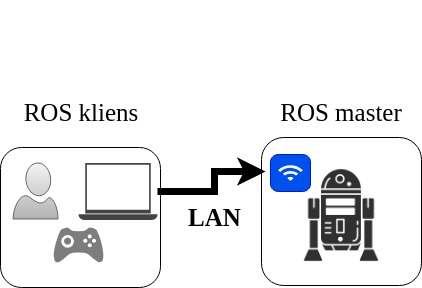
\includegraphics{tikz/RobotUserLan.jpg}
  \caption{Robothoz csatlakozás a Wifi-n keresztül.}
  \label{fig:RobotUserLan}
\end{figure}


Az \ref{fig:ROSgraph} láthatóak a főbb nodok, topikok és a köztük levő relációk. A nodok és a topikok leírását a \ref{Tab:nodok}

\begin{table}[H]
\centering
\begin{tabular}{lp{3cm}p{8cm}}
\hline Node Név & Típus & Leírás \\ \hline
  /R és /L      &  FPGA
  Communication
  Modul     &  Az FPGA-val való kommunikációért felelős. Adatokat fogad/küld  a \ref{FPGAcomuSection} fejezetben leírt protokoll alapján, amelyeket továbbít a ROS operációs rendszerben működő nodoknak.     \\
  /ImuInBoxA       &    Imuxxxx   &  Feladata szöveges formában érkező adatok feldolgozása és a ROS keretrendszerbe integrálását oldja meg. Mért fizikai mennyiségek:       \\
  /WheelOdometry       &       &   Kerekek mozgásából számolt robot elméleti pozíciója a térben     \\
  /TeleopJot      &       & Feladata a joystick-től érkező parancsok fogadása. Megvalósítja a $Dead Man Switch$ gomb kezelését, létrehoz egy globálisan engedélyező jelet a /setEMS-t és a /TeleopSig-t, amely előírja a robot lineáris mozgási sebességét és a forgási sebességét a Z tengely körül.  \\
  /rplidarNode & & A lidar mérési adatait olvassa ki és továbbítja a /scan topikban.\\
  /rosserial\_server & & A megvalósítja a kommunikációt egy esp8266 fejlesztőlap és a ROS között, amely az akkumulátorok feszültségeinek a merését végzi \cite{RosSerial}.\\
  /Joy & & Joystick eszközök integrációját valósítja meg \cite{rosjoy}.\\
  /hector\_mapping & & Lidar mérései alapján 2D térképet készit a környezetről, miközben lokalizálja a robotot ezen a térképen \cite{roshectormap}\\
  /Measurement & & mérésék elvégzésére szolgáló node, amely egy élőre beállított intervallumokban a megadott referencia értékeket küld ki az FPGA ban levő szabályzóknak.\\
  /TelepoController & & Átalakítja a robot sebesség állapotait és kiszámolja nyílt hurokban a szabályzok előírt értékeit. Abban az esetben, ha a /movebase nodot használjuk, ez megoldja a robot pozíció szabályozását a térképen, így a $/cmd_vel$ csomagot csak átalakítja /refVals csomaggá azáltal, hogy azonos oldalon levő kereke ugyanazt a referencia értéket kell követniük.
  
\end{tabular}
 \label{Tab:nodok} 
\end{table}

\subsection{Üzenet típusok (.msg)}
Az alábbi táblázatban láthatjuk a ROS operációs rendszer által szolgáltatott .msg üzenetek kiterjesztését, amelyek lehetővé teszik az FPGA integrációját a ROS környezethez.
\begin{table}[H]
\centering
\begin{tabular}{lllp{6cm}}
\hline \textbf{Üzenet típus}              & \textbf{Értékek}   & \textbf{Erkek típusa} & \textbf{Leírás} \\ \hline
 header                   &     -     &      std\_msgs/Header      &   Minden üzenet tartalmaz egy fejlécet, amely információkat tartalmaz az üzenetről. \\   
                          & seq       &      uint32        &   minden üzenetet egyedileg beazonosító szám     \\
                          & stamp     &      time        &  idő-bélyeg amely a küldés idő-pillanatát tárolja.      \\
                          & frame\_id  &      string        &        \\  \hline
                          
\hline  \multirow{1}{*}{/GlobalEnable}  &   systemIsOk        &    int16          &    
                                                                          =0 - a HLC működik.
                                                                          
                                                                          <>0 -  a HLC nem nem működik      \\    \hline                    
\hline\multirow{4}{*}{/refVals} & names     & string{[}{]} &        \\
                          & ref\_position  & float{[}{]}  & előírt szög pozíció       \\
                          & ref\_velocity & float{[}{]}  &  előírt szög sebesség      \\ 
                          & ref\_effort &    float{[}{]}  &  előírt forgatónyomaték    \\\hline
 \hline \multirow{1}{*}{/setEMS}  &   value        &     int16         &      =0 - Vészleállító aktív.
                                                                          
                                                                       <>0 -  Vészleállító nem aktív  \\     \hline 
\hline\multirow{3}{*}{/joyControll} & vx     & float64 &    A robot X tengely mentén előírt sebessége m/s-ban.    \\
                          & omega  & float64  & előírt szög pozíció   A robot Z tengely körüli forgása \degree/s-ban.    \\
                          & ControlMode & int64  &  Választhatunk a HLC szabályzok típusa vagy a manuális irányítás közül 
                           =0 move\_base szabályzó, =1 manuális irányítás joystick segítségével.\\   \hline                                                                       
\end{tabular}
\end{table}

A \ref{fig:ROSgraph} ábrán láthatjuk a nodok és az üzenetek közti kapcsolatot.

\renewcommand{\img}{SajatRobot/ROS/rosgraph.svg}
\renewcommand{\sources}{*}
\renewcommand{\svg}{svg}
\renewcommand{\aspectratioPic}{1.4}
\renewcommand{\rotationAnglePic}{90}
\renewcommand{\captionn}{ROS graph}
\renewcommand{\figlabel}{ROSgraph}
\begin{kep}
\begin{figure}[H]
\centering
\ifthenelse{\equal{\svg}{*}}
{
    \includegraphics[width=\aspectratioPic\textwidth,angle=\rotationAnglePic]{\img}
}
{
    \includesvg[width=\aspectratioPic\textwidth,angle=\rotationAnglePic]{\img}
}

 \ifthenelse{\equal{\sources}{*}}
    { \captionof{figure}{ \captionn}}
    { \captionof{figure}{ \mand{\mand{\captionn}{Forrás:}}{}} }
  	

\ifthenelse{\equal{\figlabel}{*}}
    {}
    {\label{fig:\figlabel}}%
    
\renewcommand{\figlabel}{*}



\end{figure}
\end{kep}
\renewcommand{\aspectratioPic}{1}
\renewcommand{\rotationAnglePic}{0}
\renewcommand{\svg}{*}


\subsection{FPGA kommunikációs modul ROS oldali integració}

A ROS biztosít a fejlesztőknek egy megoldást, amelyek képesek újonnan létrehozott robot integrálását ROS környezetben \cite{RosSerial}. Előnye hogy gyorsan látványos eredményt érhetünk el, de a működés sebességben és az üzenetek méretében is korlátozott. Ezen hátrányokból kifolyólag sajátos integráció szükséges, amely integrálta az FPGA UART kommunikáció protokollt a ROS keretrendszerben működő más modulokhoz.

A \ref{fig:ROStoUart} diagramon a kommunikáció node technikai megvalósítását láthatjuk. Különálló szál gondoskodik az UART adatok olvasasáról és írásáról. Az üzenetek értelemezését egy külön szál végzi és hívja fel a kiszolgáló függvényeket.
A paraméterek helyes beállításáról a ParamThread szál gondoskodik, paraméterek helyes beállításáról FPGA oldalon. Abban az esetben, ha a hardver kap egy űj paramétert a \ref{fig:MicroblazeSoft} alapján az FPGA visszaküldi a kapott paramétert, a visszajelzésből eldönthető, hogy a paraméter  a hardverben helyesen állítódott e be. Abban az esetben, ha nem megfelelő, újraküldődik mindaddig amíg nem sikeres a beállítás.

A paraméterek kezelésére a ROS paraméter szerver a felelős \cite{parameterserver}, abban az esetben, ha egy paraméter megváltozott, amely az illető nodehoz köthető, akkor a \ref{fig:ROStoUart} ábrán látható ParameterValtozott esemény előidézi a  megváltozott paraméter értékének az elküldését  FPGAnak irányába.

A globális engedélyező jel a \ref{fig:ROStoUart} MasterLive Enable,  /globalEnable típusú üzenettel engedélyezhetjük a szabályzok működését, a folyamatos működéshez 500ms periódussal kell érkeznie. Abban az esetben, ha a központi számítógép valami okból leállna, akkor a hardveres szabályzok is leállnak. A node 300ms periódussal küldi tovább az engedélyező jelet az FPGA modulnak. A HardverLive jel információt szolgáltat a többi ROS környezetben futó és a működés szempontjából kritikus nodenak, hogy az adott modul megfelelően működik e. Ezen információ birtokában a HeartBeat node leállítja a rendszert, ha egyik FPGA modul nem válaszol.

\renewcommand{\img}{SajatRobot/ROS/NodeUML.jpg}
\renewcommand{\sources}{*}
\renewcommand{\captionn}{ROS integrálása Uart protokolhoz.}
\renewcommand{\figlabel}{ROStoUart}
\begin{kep}
\begin{figure}[H]
\centering
\ifthenelse{\equal{\svg}{*}}
{
    \includegraphics[width=\aspectratioPic\textwidth,angle=\rotationAnglePic]{\img}
}
{
    \includesvg[width=\aspectratioPic\textwidth,angle=\rotationAnglePic]{\img}
}

 \ifthenelse{\equal{\sources}{*}}
    { \captionof{figure}{ \captionn}}
    { \captionof{figure}{ \mand{\mand{\captionn}{Forrás:}}{}} }
  	

\ifthenelse{\equal{\figlabel}{*}}
    {}
    {\label{fig:\figlabel}}%
    
\renewcommand{\figlabel}{*}



\end{figure}
\end{kep}
\renewcommand{\aspectratioPic}{1}
\renewcommand{\rotationAnglePic}{0}
\renewcommand{\svg}{*}


\subsection{Előirt értékek}
A /refVals típusú üzenetben megadjuk minden egyes motor előírt értékét annak fövenyében $\degree/s$ hogy sebesség alapján szabályzunk vagy $N/m$ előírt nyomaték alapján.


\subsection{Vonatkoztatási Rendszerek }
A  vonatkoztatási rendszerek szükségesek, mert a szenzorok és beavatkozó eszközök egymáshoz viszonyított helyzete és poziciója is változhat. Sok esetben szükséges ismernünk egy adott eszköznek a múltbeli helyzetét, vagy egy másik vonatkoztatási rendszerhez képest a pozícióját vagy irányát. A ROS biztosít egy tf \cite{rosTF} nevű csomagot amely megvalósítja a szűkséges transzformálásokat a $VNR$-k között. 
A \ref{fig:ROSframes} látható a kialakított vonatkoztatási rendszerek a roboton amely hűen modellezi a fizikai robot kialakítását.
A vonatkoztatási rendszereket két csoportba oszthatók:

\begin{enumerate}[label=(\alph*)]
\item rögzített pozíció és szögek, szabadságok 0:
Szenzorok laser, BODY\_link, wheel\_odom, ImuALink VNR je a base\_link a globális robot VNR hoz:
\item rögzített pozíció csak szögek változnak, szabadságok 1: Kerekek VNR je: FL\_link, BL\_link, FR\_link, BR\_link a BODY\_link hez képest csak Y körül foroghat.
\item pozíció és szög is változik, szabadságok 6:
A robot base\_link az helymeghatározás odom, és az odometria a térképhez map viszonyítva.
\end{enumerate}


A robot modellt ROS környezetben URDF robot leíró, xml alapú fájlal tehetjük meg, \cite{rosURDF}
\cite{rosJoint} \cite{rosLink}.
Az <origin> tag az xzy paraméter alatt, megadhatjuk a csukló pozícióját mindhárom tengelyen, méterben kifejezve a <parent> tagban szereplő linkhez képest. Az rpy paraméter alatt az elfordulásokat rendre x, y, z tengelyek mentén radiánban kifejezve.
Az <axis> tagban beállíthatjuk a kényszereket, jelen esetben csak az y tengely körüli forgás engedélyezett, azaz a kerekek esetében. 
Az <link> tagban robot elemeket hozhatunk létre. Az alábbi XML-ben látható a robot fizikai leírása, amely megfelel a valós szerkezetnek.
\begin{lstlisting}[language=XML]
<robot name="mobile_robot_platform_4Wheel">
	<link name="base_link" > </link>
	<link name="FL_link" > </link>
	<link name="BR_link" > </link>
	<link name="BL_link" > </link>
	<link name="BODY_link"> </link>  
	<link name="ImuALink"> </link>  
	<link name="laser"> </link> 

	<joint name="FL" type="continuous">
		<parent link="BODY_link"/>
		<child link="FL_link"/>    
		<origin xyz="0.29 -0.33 0" rpy="0 0 0" />
		<axis xyz="0 1 0" />
	</joint>

	<joint name="FR" type="continuous">
		<parent link="BODY_link"/>
		<child link="FR_link"/>    
		<origin xyz="0.29 0.330 0" rpy="0 0 0" />
		<axis xyz="0 1 0" />
	</joint>

	<joint name="BL" type="continuous">
		<parent link="BODY_link"/>
		<child link="BL_link"/>
		<origin xyz="-0.29 -0.330 0" rpy="0 0 0" />
		<axis xyz="0 1 0" />
	</joint>

	<joint name="BR" type="continuous">
		<parent link="BODY_link"/>
		<child link="BR_link"/>     
		<origin xyz="-0.29 0.330 0" rpy="0 0 0" />
		<axis xyz="0 1 0"/>
	</joint>

	<joint name="imuAandGPS" type="fixed">
		<parent link="base_link"/>
		<child link="ImuALink"/>
		<origin xyz="0.125 0.03 0.11" rpy="0 0 0" />
	</joint>

	<joint name="laserAJoin" type="fixed">
		<parent link="base_link"/>
		<child link="laser"/>
		<origin xyz="0.39 -0.02 0.23" rpy="0 0 3.14" />
	</joint>  

	<joint name="contact" type="fixed">
		<parent link="base_link"/>
		<child link="BODY_link"/>
	</joint> 
</robot>
\end{lstlisting}

A \ref{fig:ROSframes} láthatjuk, hogy a robot törzsét a $BODY\_link$ alkotja, amelyhez kapcsolódnak a kerekek: $BL\_link,FL\_link,BR\_link,FR\_link$. A $base\_link$ és a $BODY\_link$ egybe esnek. A szenzorok a $laser$, amely a lidarnak felel meg, $ImuALink$ IMU szenzor ezek a $base\_link$-hez kapcsolódnak.
A $map$ VNR a térképnek, amelyen meghatározzuk a robot pozícióját $odom$.

\renewcommand{\img}{SajatRobot/ROS/frames.svg}
\renewcommand{\sources}{*}
\renewcommand{\svg}{svg}
\renewcommand{\aspectratioPic}{1.5}
\renewcommand{\rotationAnglePic}{90}
\renewcommand{\captionn}{A megvalósított robot VNR-k közti reláció }
\renewcommand{\figlabel}{ROSframes}
\begin{kep}
\begin{figure}[H]
\centering
\ifthenelse{\equal{\svg}{*}}
{
    \includegraphics[width=\aspectratioPic\textwidth,angle=\rotationAnglePic]{\img}
}
{
    \includesvg[width=\aspectratioPic\textwidth,angle=\rotationAnglePic]{\img}
}

 \ifthenelse{\equal{\sources}{*}}
    { \captionof{figure}{ \captionn}}
    { \captionof{figure}{ \mand{\mand{\captionn}{Forrás:}}{}} }
  	

\ifthenelse{\equal{\figlabel}{*}}
    {}
    {\label{fig:\figlabel}}%
    
\renewcommand{\figlabel}{*}



\end{figure}
\end{kep}
\renewcommand{\aspectratioPic}{1}
\renewcommand{\rotationAnglePic}{0}
\renewcommand{\svg}{*}



\section{Kerekek Pid Szabalyzo hangolas}

A pid, a legelterjedtebb szabályozó egyszerű feladatok elvégzésére, esetünkben is elegendő a kerekek szögsebesség szabályzására kerekenkénti egy PID szabályzóval. A PID szoftveresen fut a uBlaze processzoron. Bemenete egy előírt forgási sebesség \degree/s ban és kimenete egy -32000 és 32000 egész típusú értek. A kimenti érteke a PWM kitöltési tényezőt jeleni, az előjel pedig a beavatkozás irányát.
Matlab/Simulink környezetben használva a Robotix Toolbox segítségével direkben pwm beavatkozo referenica erteket irtam elo a motroknak. A beavatkozó jel előállítása és elküldési a fizikai eszköznek 0-100\%-ig 10\% lépcsőkben amelyek 0\% kitoltesekkel vanak megszakitva. A mert adatokat rosbag csomagba mentve majd a System Identification Toolbox használatával identifikáljuk a rendszer modellt. A rendszer bemenete egy beavatkozójel ami fizikailag feszültségnek fele meg 0V és 12V között. A kimenetek a forgási sebesseg.
A mert adatokat Matlab/System Identification hasznalataval megbecsuljuk a rendszer modeleket. Nemlinearis modelt becslunk 
Hammerstein-Wiener model \cite{matlabhwmmodel} hasznalva, 1 kimenet es 1 bemenet, a linearis atviteli fugveny fokszama:
zerusok nb = 2, polusok nf = 3, keses a bemenet es a kimenet kozott nk = 1. A becsult adatok 94\% ban megfelelnek a mert rendszernek.          

A mereseket a robot kerekei es a talaj erintekzese nelkul vegeztem.
A becsult modelt a bemenet 50/\%  korul linearizaljuk es a linearizalt modelbol atviteli fugvenyt kesztunk. 
$tf = tf(linearize(model,16000));$ utasutast hasznalva Matlab kornyezetben. A linearizalt modelt Matlab/PidTuning eszkozt hasznalva behangolunk kiszamitjuk a megfelelo PID szabalyzo parametereit.

\input{SajatRobot/PIDHangolasa/MeasuremetSimulinkWheel.tex}

A becsült rendszer átviteli függvénye $H_s(z)$, mintavetelezesi periódus Ts: = 0.05s.

\subsection*{Nagyobik fokozatban}

A becsult modelt oszehasonlitva a mert ertekekkel a \ref{fig:NFsysIdent}, a model nemlinearis becsult model megfelel a mert ertekeknek.

\begin{figure}[H]
  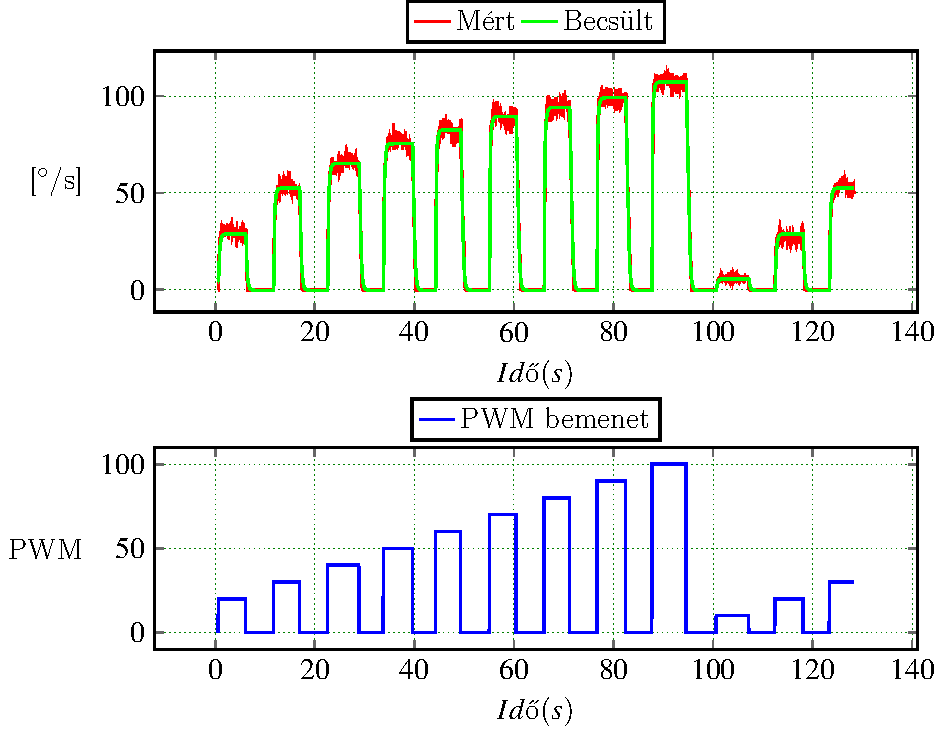
\includegraphics{tikz/NFsysIdent.pdf}
  \caption{Nagy fokozat Hammerstein-Wiener becsult model valasza, es a mert ertekek.}
  \label{fig:NFsysIdent}
\end{figure}


Az atviteli fuggveny a bemenet 50/\% korul linearizalva.

\begin{equation}
    H_s(z)=\frac{-0.07017z^{-2} -0.053z^{-1}}{-0.2117^{-3}+0.7321z^{-2} -1.393z^{-1} +1}
\end{equation}

A tervezett PID szabályozó paramétere Kp: 7.11 , Ti: 23.66 , Td: 0.43

\subsection{Kisebik fokozatban}

A becsult modelt oszehasonlitva a mert ertekekkel a \ref{fig:KFsysIdent}, a model nemlinearis becsult model megfelel a mert ertekeknek.


\begin{figure}[H]
  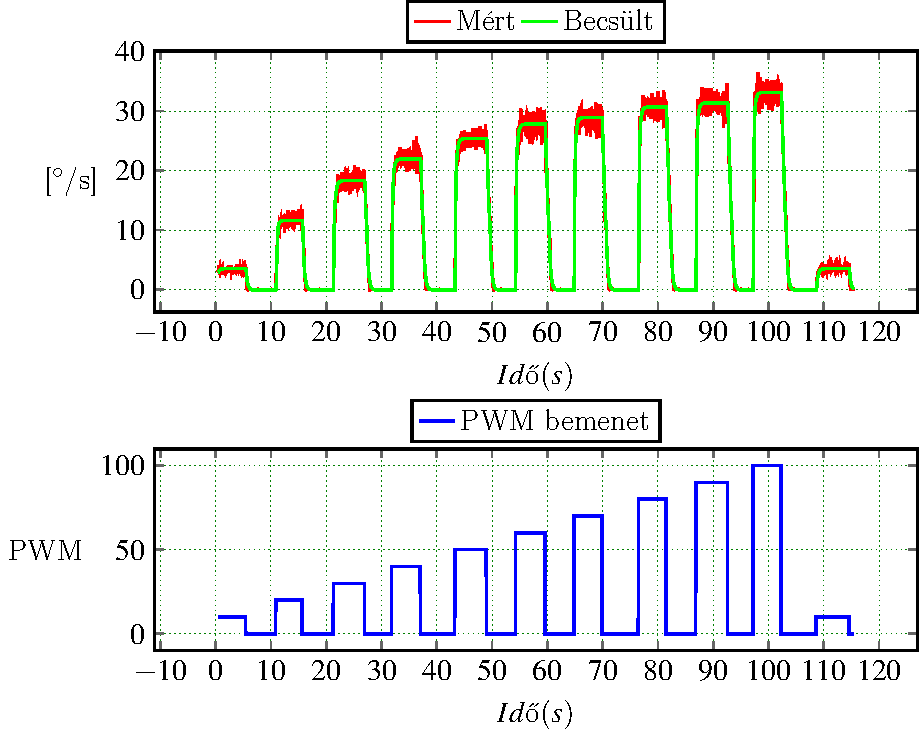
\includegraphics{tikz/KFsysIdent.pdf}
  \caption{Kis fokozat Hammerstein-Wiener becsult model valasza, es a mert ertekek.}
  \label{fig:KFsysIdent}
\end{figure}

Az atviteli fuggveny a bemenet 50/\% korul linearizalva.

\begin{equation}
    H_s(z)=\frac{-0.0291z^{-2} -0.009263z^{-1}}{-0.198z^{-3}+0.7058z^{-2} -1.394z^{-1} +1}
\end{equation}

A tervezett PID szabályozó paraméterek: Kp: 15.96 , Ti:51.51 , Td:1.237 

.



\newpage
\section{Pályakövetési feladatok}

A robot pályakövetési feladatát megfogalmazhatjuk úgy, hogy tudjunk eljutni A pontból B pontba, ha ismerjük a robot síkbeli pozícióját és az orientációját egy térképen, amely megfelel a környezetnek, látható az \ref{fig:PositionController} ábrán.
A \ref{fig:PositionController} ábrán látható, hogy felveszünk egy pozitív és egy negatív irányt a szögre nézve, az orientációkat mindig [0\degree 360\degree] között kell megadjuk. A robotnak mindig arra kell fordulnia, amerre a szög a legkisebb, azért, hogy minél kevesebbet keljen mozogjon.
A kiinduló állapotban a robot kezdetben az A pontban van és az orientációja $\beta_0$ és a B pontba szeretnénk eljutni egyenes vonalban. Így a robotnak kezdetben a célra kell fordulnia és ezután haladhat előre, miközben korrigálja az orientációs hibákat.
Első lépésben a robotnak fordulnia kell $error$ szöget, hogy $\beta_1$ irányba mutasson és ezután haladhat a cél fele.


\begin{figure}[H]
    		%trim = bal also jobb felso
   \fbox{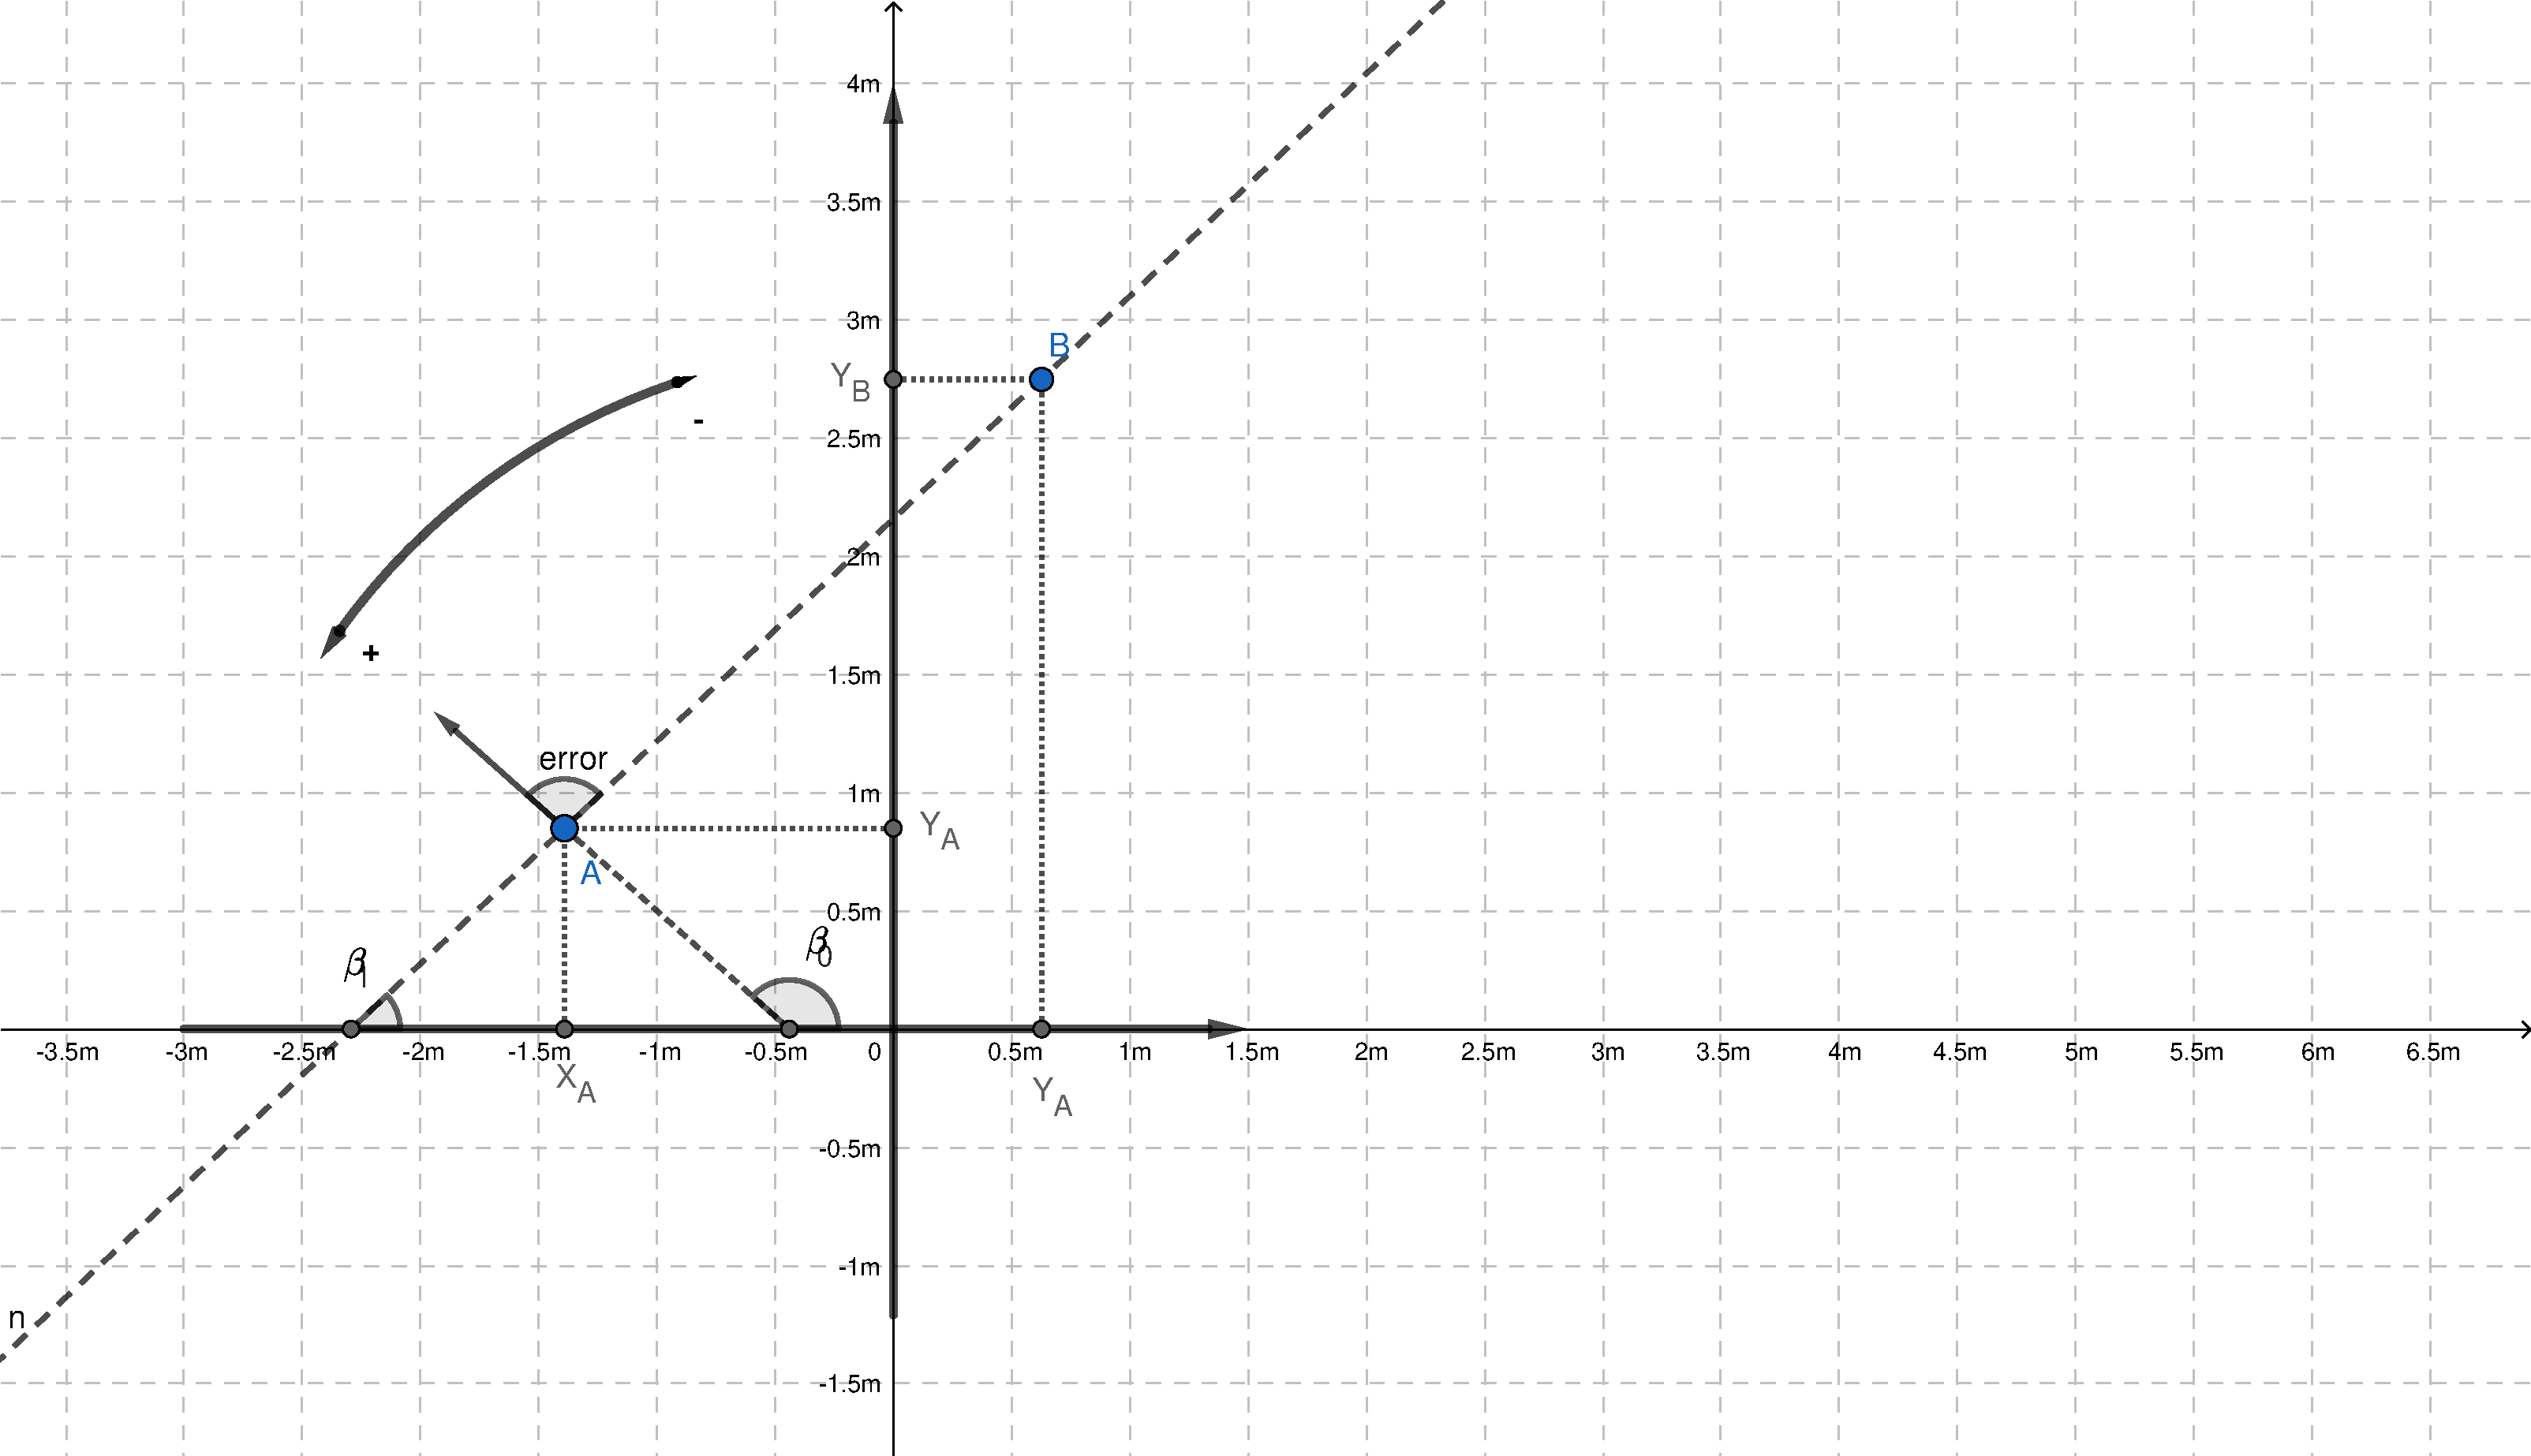
\includegraphics[width=1\columnwidth,trim=3cm 6cm 27cm 2cm,clip]{tikz/PositionController.pdf}}
  \caption{Robot pozíció szabályzása}
  \label{fig:PositionController}
\end{figure}


A pályakövetési algoritmus látható alább. Az  előírt irányt $tan^{-1}$ függvény segítségével határozzuk meg, ismerve X és Y tengelyen a hibák nagyságát. A Rotate($e_\alpha$,$\Omega_{max}$) függvényben alkalmazunk egy PI típusú szabályzót, melynek a feladata a szöghiba 0-hoz való közelítése. A Vx(d,$V_max$) a robot lineáris sebességének a szabályzását látja el egy PI típusú szabályzó, célja a robot és a kitűzött cél távolságának a csökkentése. 
A távolságszabályzó bemenetét súlyozzuk $1/e_\alpha$ értékkel, hogy ameddig nincs a robot irányban, addig ne domináljon távolságszabályzó.

\begin{algorithm}
   \caption{Pályakövetés Algoritmusa}
    \begin{algorithmic}[1]
     %\Function{GetNextControl}{$X_a,Y_a\alpha$}
      \Function{GetNextControl}{$X_a,Y_a,\alpha_a,X_t,Y_t,\alpha_t,Tr,Tr_\alpha,\Omega_{max},V_{max}$}
      %\Comment{Ahol X,Y - pozicio a térképén, \alpha irány, a - aktuális, t - előírt, Tr - pozicio hiba küszöb, $Tr_{\alpha}$ - szöghiba küszöb,${\Omega}_{max}$ maximális forgási sebesseg, $V_{max}$ maximális haladási sebesség. }
      
       \State $e_x = X_a-X_t$
       \State $e_y = Y_a-Y_t$
       \State $d=\sqrt{e_x^2+e_y^2}$
       \State $\alpha_i=dir(X_a,Y_a,X_t,Y_t)$ \Comment{Két ponton átmenő egyenes iránytényezője}
       \State $e_\alpha=\alpha_i-\alpha_a$
            \If {$e_\alpha > Tr_\alpha$} \Comment{Fordulj a cél fele}
                \State $\Omega = Rotate(e_\alpha,\Omega_{max}) $
                \State $V_x = 0 $
            \Else \Comment{Haladj a cél fele és korrigáld az elfordulást}
                
                \State $\Omega = Rotate(e_\alpha,\Omega_{max}) $
                \State $V_x = Vx(d*1/e_\alpha,V_{max})$
            \EndIf
     
            \If {$e_\alpha < Tr_\alpha$ és $d<Tr$} \Comment{Kívánt pozícióban}
                \State $\Omega = 0$
                \State $V_x = 0 $
            \EndIf
        
       \EndFunction

\end{algorithmic}
\end{algorithm}



Az algoritmus tesztelésére MATLAB/Simulink környezetet használtam. A robot kinematikai modellt az \ref{eq:allapot} egyenlet alapján modelleztem, a pozíciók (X,Y) és az irány meghatározására integráltam a lineáris és szögsebességeket. 

A \ref{fig:SimPoseCont} ábrán láthatjuk a szimulációs eredményeket, amint a robot egy végtelen jelhez hasonló pályát követ.

\begin{figure}[H]
	\setlength{\fboxsep}{0pt}
	\setlength{\fboxrule}{0pt}
	
    \begin{center}  	
    		%trim = bal also jobb felso
    	\fbox{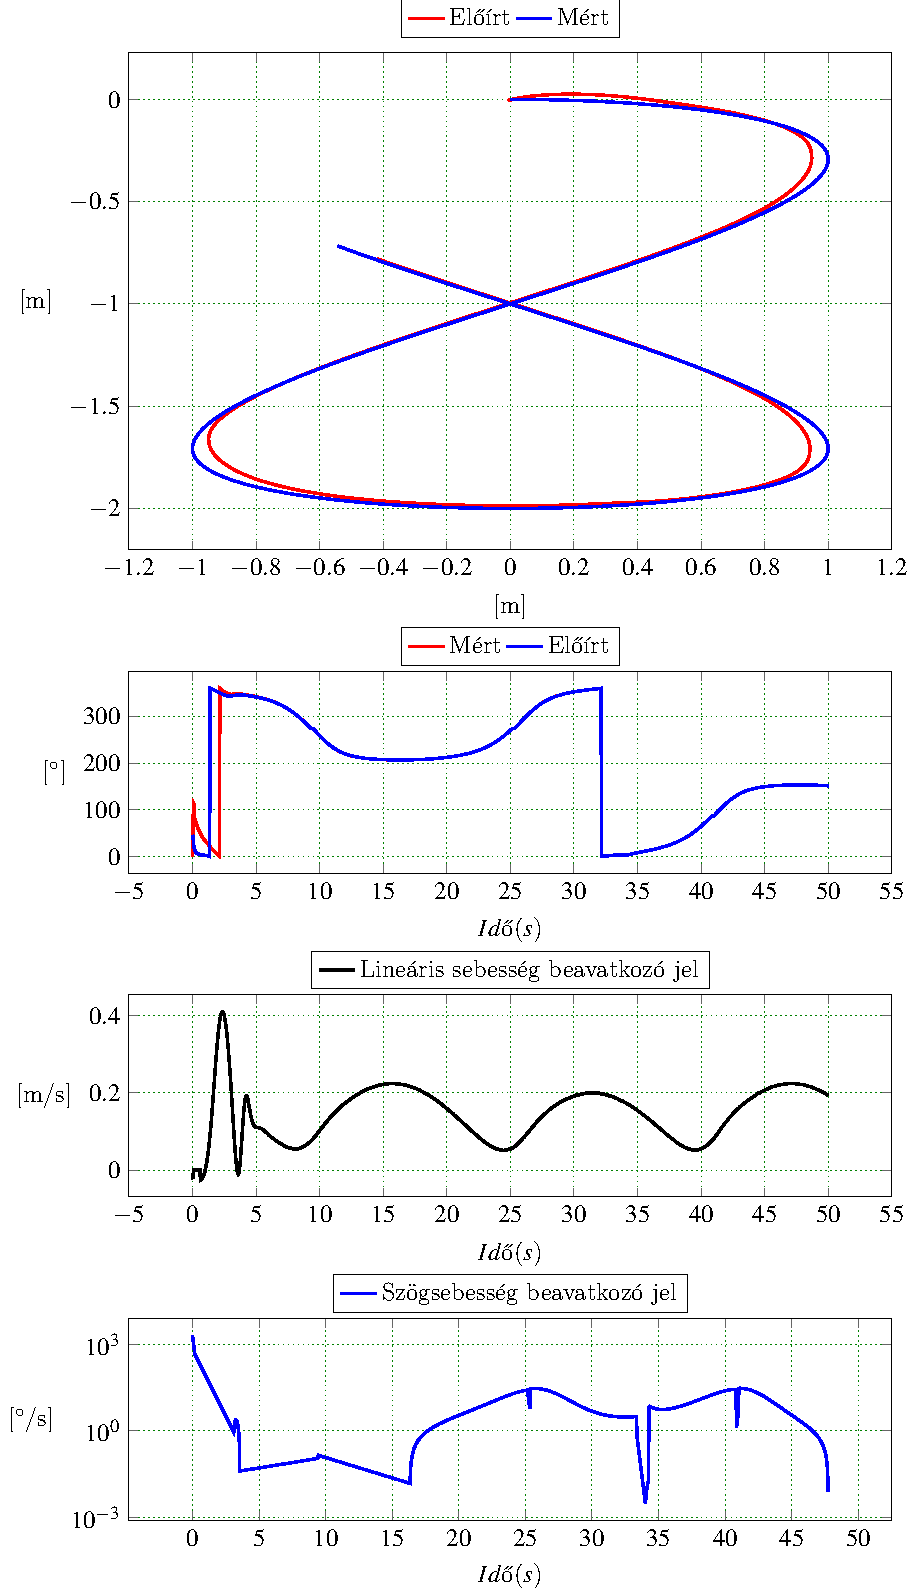
\includegraphics[width=0.9\columnwidth,trim=0cm 0cm 0cm 0cm,clip]{tikz/SimPoseCont.pdf}}
    \end{center}  
    
  	\caption{Robot pozíció szabályzása}
  	\label{fig:SimPoseCont}
\end{figure}

\newpage

\lhead{Meresek a Robottal}
\section{Meresek}
Ebben a fejezetben tanulmányozásra kerül a robot viselkedése abban az estekben ha valamely kerék meghibásodik, és ezáltal nem megfelelően működik.
Hasonló eset történt a Marson a Spitit mars roverrel (2006,Március,13) \cite{SpititWheel1} amikor az első jobb kereke meghibásodott. A megoldás az volt hogy a robot mozgása optimálisabb lesz energia felhasználás szempontjából ha háttal megy. Az energia ellátása is véges volt, kiszolgáltatott volt a napsütésnek,a nap elemekre rakodót por miatt csökkentek a ayok hatásfoka így sokkal alaposabb mozgás pálya tervezésre volt szükség.
Problémák adódtak a homokos talajjal is, a Spirit mars járonak, kerekei a homokba süllyedtek és beragadtak, a földi irányító csoport egy másolat segítségével próbálta kimozdítani a csapdaból.
A hasonló eseteket elkerülhetők lennének, ha ismerve a robot korlátait olyan mozgás pályát határoznak meg amellyel elkerulhetjuek ezen akadajokat, vagy időben detektálhatjuk ezen problémákat pl: homokba süllyedés érzékelése.


A robottal a következő méréseket fogjuk elvégezni:
\begin{enumerate}[label=(\alph*)]
\item BL kerék blokált
\item BL és BR kerék blokált
\item BL kerék maximálisan pörög
\item BL és BR kerék maximálisan pörög
\end{enumerate}


\subsection{Differenciális Forgás Vízszintes Talajon}

Diferencialis forgasnak nevezuk azt amikor a jobb es ball oldali kerekek sebesege megegyezo, csak iranyukban elenkezo, igy a robot belso teruleten belul jon letre a ICR pont a COG kozeleben kelene legyen \ref{fig:SMR4WKinematics}. 


%%globalis paremeterek a meresek kirajzolasahoz.

\pgfplotstableset{%
    x index=0,
    y index=1,
    header=true
}%

\pgfplotsset{every axis/.append style=
    {
        font=\large,
        line width=1.2pt,
        tick style={line width=0.8pt}
    }
}

\pgfplotsset{
    contour/every contour label/.style={
    sloped,
    transform shape,
    inner sep=1pt,
    every node/.style={mapped color!50!black,fill=white},
    /pgf/number format/relative={\pgfplotspointmetarangeexponent},
    },
}






\subsection{Feloldali kerekek blokolva kavicsos talajon}

A robot baloldali kerekei leblokkolva és a jobboldali kerekei 50\degree/s szögsebességgel forognak. Az eredmények alapján a \ref{fig:Left0Right50b} látható a robot által leírt pálya. A mozgás során több mint 360 \degree -t fordul és mondhatni körpályát írt le. A talajjal való súrlódások miatt a robot nem tökéletesen fordul ez látható abból is hogy a másodszori fordulás már az előzőhöz képest más középponttal rendelkezik. 

\renewcommand{\GlobalPath}{Meresek/Mozgasok/HibasMukodes/R_0_L_1/}
\renewcommand{\secondImage}{*}

%kep a talajrol
%

\renewcommand{\sources}{}
\renewcommand{\captionn}{Kep a felszinrol}
\renewcommand{\figlabel}{figm}


\begin{kep}
    \begin{figure}[H]%
    \begin{center}
    
    \subfloat[label a]{
        {\includegraphics[width=9cm]{\mand{\GlobalPath}{talaj1.jpg}} }
        \label{fig:ex3-a}
    }%
    
    \ifthenelse{\equal{\secondImage}{*}}
    {}
    {
        \qquad
        \subfloat[label b]{{\includegraphics[width=9cm]{\mand{\GlobalPath}{talaj1.jpg}} }}%
    }
  
    \label{fig:example}%
    \end{center}
\end{figure}
\end{kep}

\renewcommand{\secondImage}{*}



%1
% %1
    \begin{figure}
    
        %-------------------------------------------------Joint Adatok---------------
        \begin{subfigure}{\textwidth}
            \begin{center}
        
            \input{\mand{\GlobalPath}{L.tex}}
            \pgfplotstableread{NodeLeft.dat}{\leftNode}

            
            \input{\mand{\GlobalPath}{R.tex}}
            \pgfplotstableread{NodeRight.dat}{\rightNode}

        
            \begin{tikzpicture}
            \pgfplotsset{every axis plot/.append style={very thick}}
            \setcaptionsubtype
            
            % megjelenites beallitasai
            
            \begin{groupplot}[%
                        ,group style={%
                            ,group name=my plots
                            ,group size=2 by 2
                            ,vertical sep=1.8cm,
                            ,horizontal sep = 2.4cm,
                            ,ylabels at=edge left
                        }
                        ,width=7cm
                        ,height=6cm
                        ,try min ticks=5
                        ,xlabel={\bfseries{\emph{\idoFelirat}}}
                        ,zlabel={\bfseries{\emph{kg}}}
                        %%ha kell y felirat az elso ketore
                        %,ylabel={\bfseries{\degree$/s$}}
                        %,ylabel style={rotate=-90}
                        %,xtick={0,10,...,60},
                        %,minor tick num=5
                        %,xtick distance=10
                        %,ytick distance=25
                        ,grid=major%both
                        ,every both grid/.style={gray, opacity=0.7},
                        view={0}{90},
                        legend columns=2,
                        %xmin=0,xmax=0.65,
                        %ymin=0,ymax=0.65,
                       % zmin=-5,zmax=60,
                        ]
            %% ide jonnek a adatok. 
            
            %ha kell felirat be kell teni a nextplot[] parameterei koze
            % \nextgroupplot[ylabel=\degree$/s$, ylabel style={rotate=-90},legend to name={CommonLegend},legend style={legend columns=2}]
            \nextgroupplot[]
                \addplot [color=green,each nth point={\nth}] table [header=true, x=Time, y=refOmegaA] {\leftNode};\label{plots:plot3}
                \addplot [color=black,each nth point={\nth}] table [header=true, x=Time, y=effortA] {\leftNode};\label{plots:plot4}
                \addplot [color=blue,each nth point={\nth}] table [header=true, x=Time, y=omegaA] {\leftNode}; \label{plots:plot1}
                \addplot [color=red,each nth point={\nth}] table [header=true, x=Time, y=pwmA] {\leftNode};\label{plots:plot2}
                \coordinate (top) at (rel axis cs:0,1);% coordinate at top of the first plot
            
            \nextgroupplot[]
                \addplot [color=green,each nth point={\nth}] table [header=true, x=Time, y=refOmegaA] {\rightNode};
                \addplot [color=black,each nth point={\nth}] table [header=true, x=Time, y=effortA] {\rightNode};
                \addplot [color=blue,each nth point={\nth}] table [header=true, x=Time, y=omegaA] {\rightNode};
                \addplot [color=red,each nth point={\nth}] table [header=true, x=Time, y=pwmA] {\rightNode};
                    
            \nextgroupplot[]
                \addplot [color=green,each nth point={\nth}] table [header=true, x=Time, y=refOmegaB] {\leftNode};
                \addplot [color=black,each nth point={\nth}] table [header=true, x=Time, y=effortB] {\leftNode};
                \addplot [color=blue,each nth point={\nth}] table [header=true, x=Time, y=omegaB] {\leftNode};
                \addplot [color=red,each nth point={\nth}] table [header=true, x=Time, y=pwmB] {\leftNode};
                   
            \nextgroupplot[]
                \addplot [color=green,each nth point={\nth}] table [header=true, x=Time, y=refOmegaB] {\rightNode};
                \addplot [color=black,each nth point={\nth}] table [header=true, x=Time, y=effortB] {\rightNode};
                \addplot [color=blue,each nth point={\nth}] table [header=true, x=Time, y=omegaB] {\rightNode};
                \addplot [color=red,each nth point={\nth}] table [header=true, x=Time, y=pwmB] {\rightNode};
                \coordinate (bot) at (rel axis cs:1,0);% coordinate at bottom of the last plot
            \end{groupplot}
            
            %\path [nodes={anchor=south,rotate=90,font=\large\bfseries,midway}]
            %  (my plots c1r1.outer north west)--(my plots c1r2.outer south west)
            %    node {Testing of Parameters 1}
            %  (my plots c2r1.outer north west)--(my plots c2r2.outer south west)
            %    node {Testing of Parameters 2};
            
            % legend
            \node[text width=.5\linewidth,align=center,anchor=south] at (my plots c1r1.north) {\caption[]{FL\label{subplot:one}}};
            \node[text width=.5\linewidth,align=center,anchor=south] at (my plots c2r1.north) {\caption[]{FR\label{subplot:two}}};
            \node[text width=.5\linewidth,align=center,anchor=south] at (my plots c1r2.north) {\caption[]{BL\label{subplot:three}}};
            \node[text width=.5\linewidth,align=center,anchor=south] at (my plots c2r2.north) {\caption[]{BR\label{subplot:four}}};
            
            %\path (top-|current bounding box.west)-- 
            %      node[anchor=south,rotate=90] {throughput} 
            %      (bot-|current bounding box.west);
            % legend
            \path (top|-current bounding box.north)--
                  coordinate(legendpos)
                  (bot|-current bounding box.north);
            \matrix[
                matrix of nodes,
                anchor=south,
                draw,
                inner sep=0.2em,
                draw
              ]at([yshift=1ex]legendpos)
              {
                \ref{plots:plot1}& Aktualis Szogsebesseg [\degree$/s$]&[5pt]
                \ref{plots:plot2}& PWM [$\%$] &[5pt]
                \ref{plots:plot3}& Eloirt Omega [\degree$/s]$
                \ref{plots:plot4}& Energia $[Watt]$ &[5pt]\\
            };
           % \centering
            \end{tikzpicture}
            \end{center}
        \end{subfigure}
        
        \iffalse
        %-------------------------------------------------Power Adatok---------------
        \newline
        \begin{subfigure}{\textwidth}
        \begin{center}
        \input{\mand{\GlobalPath}{Power.tex}}
        \pgfplotstableread{Power.dat}{\power}
        
        
        \begin{tikzpicture}
        \pgfplotsset{every axis plot/.append style={very thick}}
        \setcaptionsubtype
        
        % megjelenites beallitasai
        
        \begin{groupplot}[%
                    ,group style={%
                        ,group name=my plots
                        ,group size=1 by 1
                        ,vertical sep=2cm,
                        ,horizontal sep = 0cm,
                        ,ylabels at=edge left
                    }
                    ,width=14.5cm
                    ,height=6cm
                    ,try min ticks=5
                    ,xlabel={\bfseries{\emph{\idoFelirat}}}
                    %,ylabel={\bfseries{\emph{A}}}
                    %,zlabel={\bfseries{\emph{kg}}}
                    ,grid=both
                    ,every both grid/.style={gray, opacity=0.5}
                    ,view={0}{90},
                    %,xtick distance=10
                    %,minor tick num=5
                    %,ytick distance=5
                    %xmin=0,xmax=0.65,
                    %ymin=0,ymax=0.65,
                    %zmin=-5,zmax=60,
                    ]
        %% ide jonnek a adatok.            
                    
        \nextgroupplot[ylabel=\emph{}, ylabel style={rotate=-90}]
         \addplot [color=red,each nth point={\nth}] table [header=true, x=Time, y=voltage] {\power};\label{plots:plot11}
         \addplot [color=green,each nth point={\nth}] table [header=true, x=Time, y=current]{\power};\label{plots:plot12}
         \addplot [color=black,each nth point={\nth}] table [header=true, x=Time, y=power] {\power};\label{plots:plot13}
        \end{groupplot}
        
        %\path [nodes={anchor=south,rotate=90,font=\large\bfseries,midway}]
        %  (my plots c1r1.outer north west)--(my plots c1r2.outer south west)
        %    node {Testing of Parameters 1}
        %  (my plots c2r1.outer north west)--(my plots c2r2.outer south west)
        %    node {Testing of Parameters 2};
        
        % legend
        \node[text width=.5\linewidth,align=center,anchor=south] at (my plots c1r1.north) {\caption[]{Energia Fogyasztas\label{subplot:one}}};
        
        %\path (top-|current bounding box.west)-- 
            %      node[anchor=south,rotate=90] {throughput} 
            %      (bot-|current bounding box.west);
            % legend
            \path (top|-current bounding box.north)--
                  coordinate(legendpos)
                  (bot|-current bounding box.north);
            \matrix[
                matrix of nodes,
                anchor=south,
                draw,
                inner sep=0.2em,
                draw
              ]at([yshift=1ex]legendpos)
              {
                \ref{plots:plot11}&  Akumlator Feszultsege [V]&[5pt]
                \ref{plots:plot12}& Akkumlator Arama [A] &[5pt]
                \ref{plots:plot13}& Teljesitmeny [W] \\
            };
        
        %\centering
        \end{tikzpicture}
        \end{center}
        \end{subfigure}
        % Caption
        %\caption[]{$SSMR-4W$ tipusu robot kereknyomoerok kerekenkeni változása a sulypont fuggvenyeben}\label{abserror}
        \fi
    \end{figure}




\begin{figure}[H]
	\begin{center}
  		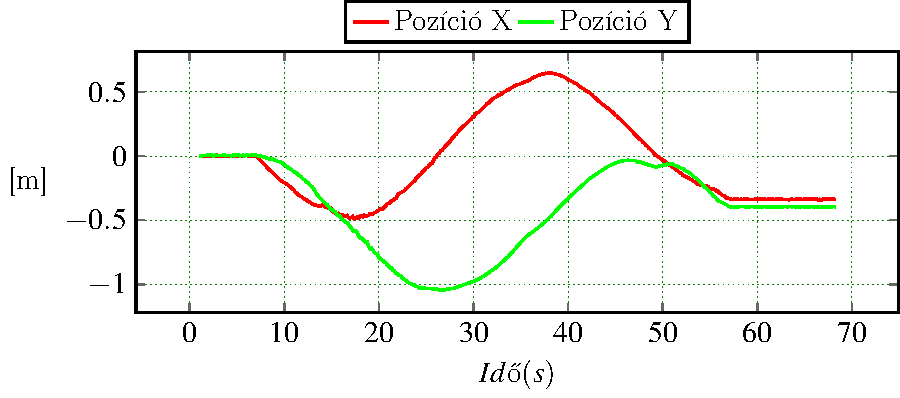
\includegraphics[scale=0.8]{tikz/Left0Right50a.pdf}
  	\end{center}
  \caption{$SSMR-4W$ típusú robot pozíciója, X és Y tengelyekre bontva, keréksebességek BL=FL=0 és a FR=BR= 50\degree/s}
    \label{fig:Left0Right50a}
\end{figure}


\begin{figure}[H]
	\begin{center}
  		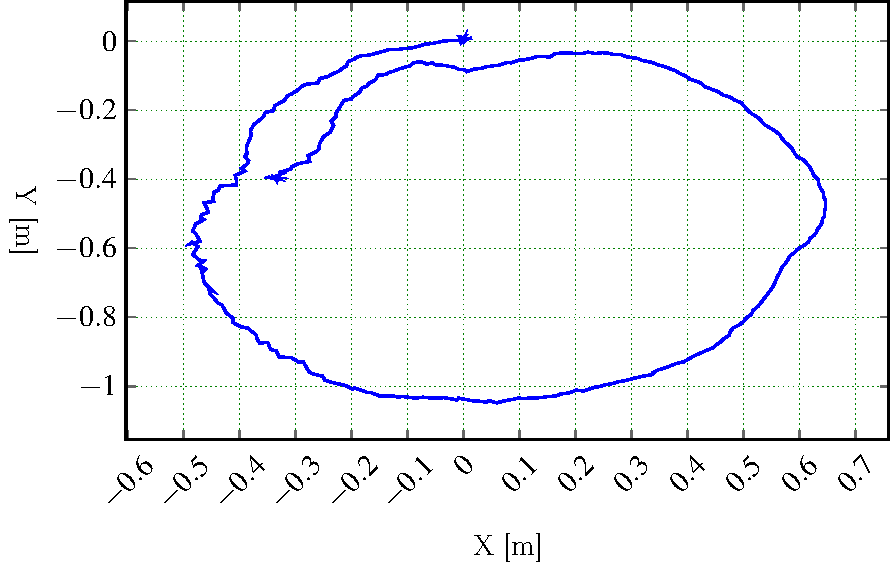
\includegraphics[scale=1]{tikz/Left0Right50b.pdf}
  	\end{center}
  \caption{$SSMR-4W$ típusú robot által leírt pálya, kerekesebességek BL=FL=0 és a FR=BR= 50\degree/s}
  \renewcommand{\figlabel}{Left0Right50b}
  \label{fig:Left0Right50b}
\end{figure}

A mérés során a fordulási szögsebesség 9\degree/s látható a \ref{fig:Left0Right50c} ábran. A LIDAR és HectorMap segítségével mért abszolut szögsebesség zajosabb mint a giroszkóp által mért. A LIDAR-al mért szögsebesség előnyösebb mert a zajokat nem kell integrálni ahhoz hogy megkapjuk a szögsebességet a giroszkóppal ellentétben.

A lineáris sebességeket tekintve \ref{fig:Left0Right50d} szinuszosan változnak, az X és Y tengelyeken, megfigyelhető egy 90\degree eltolódás az X és Y tengelyeken mért szinuszos mozgásban. A kerületi sebesség 0.1 m/s körül adható meg.

\begin{figure}[H]
	\begin{center}
  		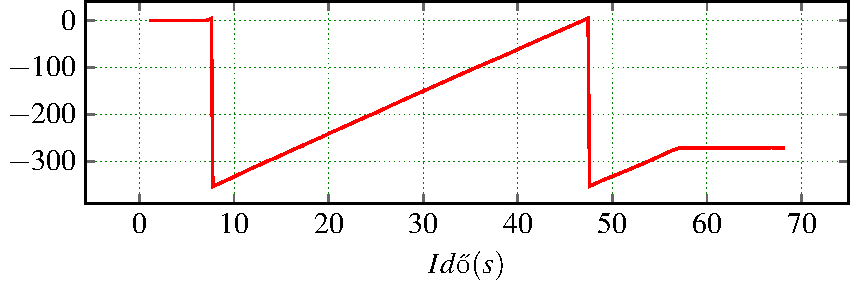
\includegraphics[scale=1]{tikz/Left0Right50c.pdf}
  	\end{center}
  \caption{$SSMR-4W$ típusú robot orientációja,ha a kerékszögsebességek BL=FL=0 és a FR=BR=50\degree/s}
  \label{fig:Left0Right50c}
\end{figure}


\begin{figure}[H]
	\begin{center}
  		\label{fig:Left0Right50d}
  		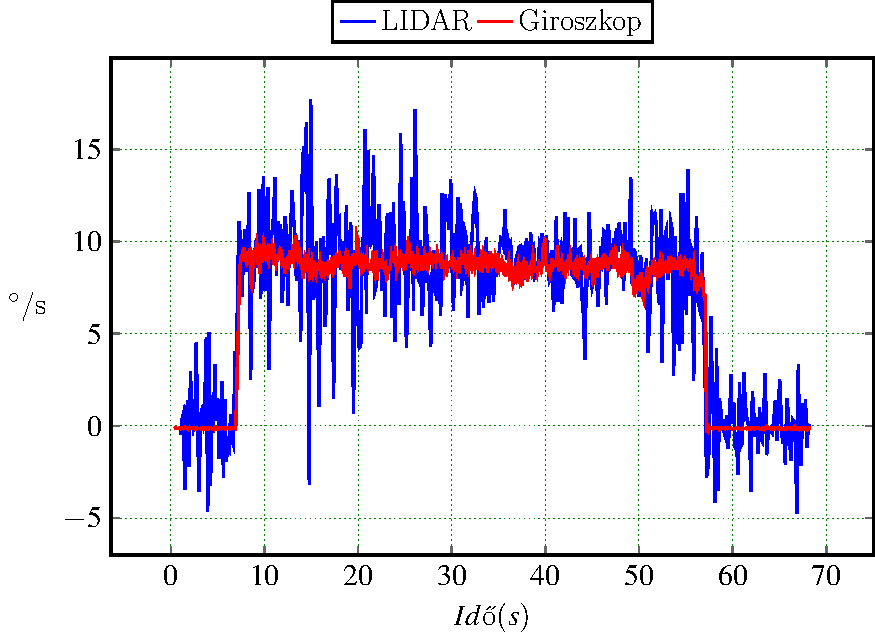
\includegraphics[scale=0.9]{tikz/Left0Right50d.pdf}
  	\end{center}
  \caption{$SSMR-4W$ típusú robot fordulási szögsebessége Giroszkóp és LIDAR által mért értékek, ha a kerékszögsebességek BL=FL=0 és a FR=BR= 50\degree/s}
  \label{fig:Left0Right50d}
\end{figure}


\begin{figure}[H]
	\begin{center}
  		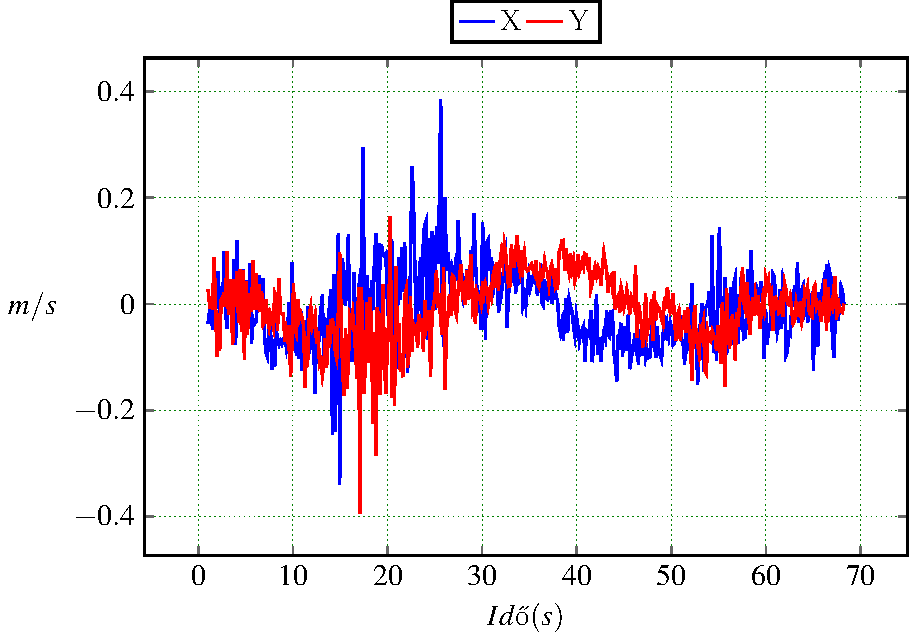
\includegraphics[scale=0.9]{tikz/Left0Right50e.pdf}
    \end{center}
  \caption{$SSMR-4W$ típusú robot súlypontjának sebessége a globális VNR-ben, X és Y tengelyekre bontva, ha a kerékszögsebességek BL=FL=0 és a FR=BR= 50\degree/s}
  \label{fig:Left0Right50e}  
\end{figure}











\subsection{Kavicsos talajon helyben forgás}
A \ref{fig:Left_n50Right50a} megfigyelhető amint a robot kavicsos talajon differenciálisan fordul 60 másodpercen keresztül, ezalatt háromszor teljen korbefordul. A palyat tekintve letrejon egy oldaliranyu mozgás is igy 0.4m kerul odebb. Az oldaliranyu mozgas a nem egyenlo surlodasok es eroeloszlasok miatt jon letre.

\renewcommand{\nth}{2}
\renewcommand{\GlobalPath}{Meresek/Mozgasok/NormalMukodes/DiferencialisanHelybeKavicsos/}
\renewcommand{\secondImage}{*}



\begin{figure}[H]
  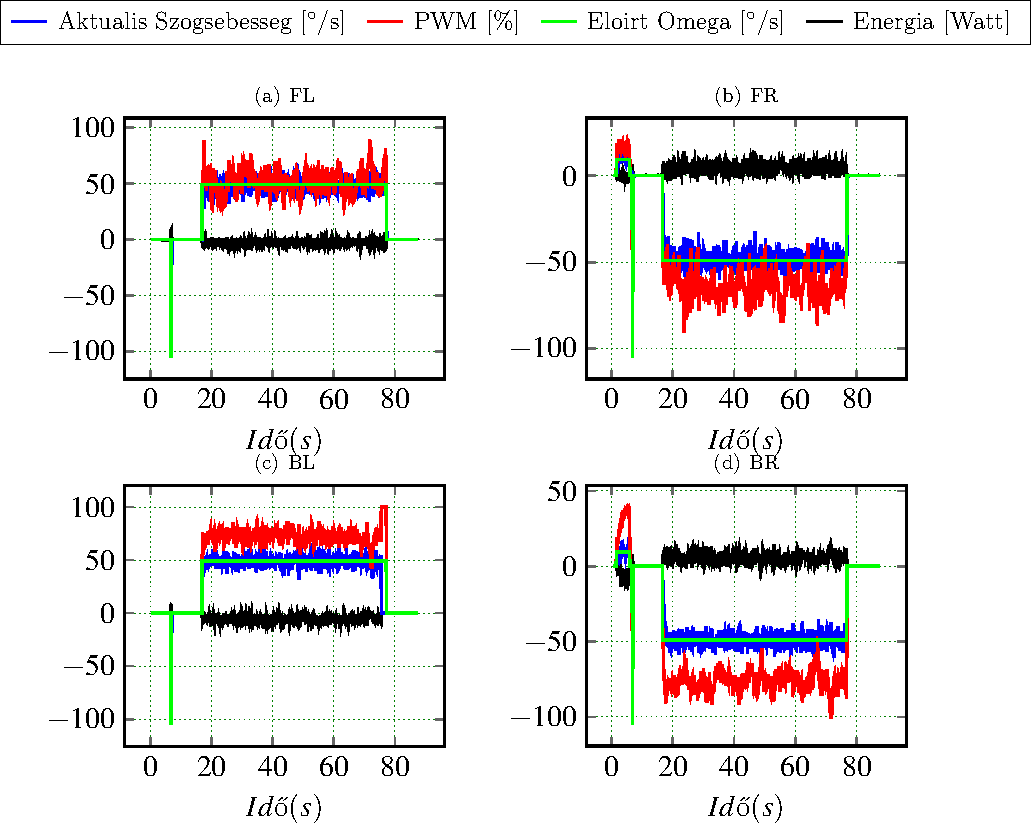
\includegraphics{tikz/Left_n50Right50x.pdf}
  \caption{$SSMR-4W$ típusú robot mozgása, tengelyekre bontva, kereksebessegek BL=FL=0 es a FR=BR= 50\degree/s}
  \label{fig:Left_n50Right50x}
\end{figure}


\begin{figure}[H]
  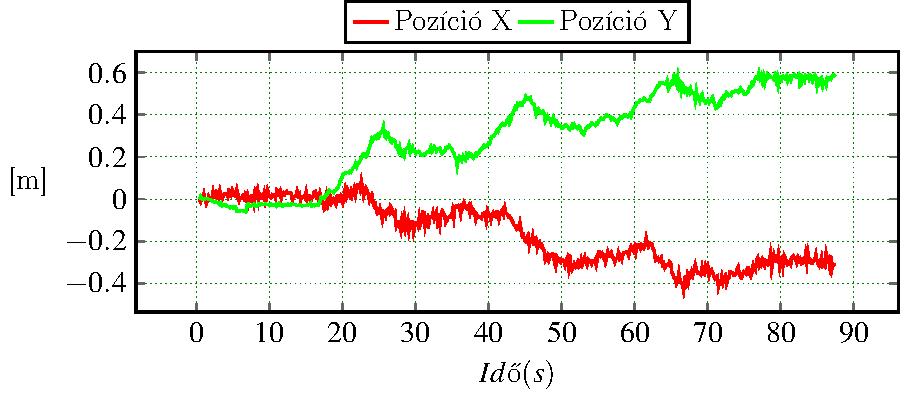
\includegraphics{tikz/Left_n50Right50a.pdf}
  \caption{$SSMR-4W$ típusú robot mozgása, tengelyekre bontva, kereksebessegek BL=FL=-50 es a FR=BR= 50\degree/s}
  \label{fig:Left_n50Right50a}
\end{figure}


\begin{figure}[H]
  \label{fig:Left_n50Right50b}
  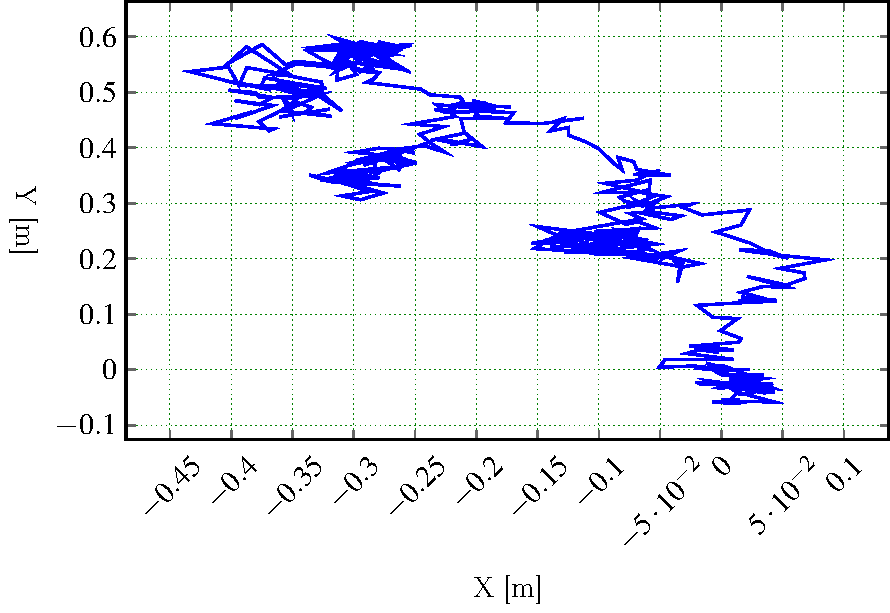
\includegraphics{tikz/Left_n50Right50b.pdf}
  \caption{$SSMR-4W$ típusú robot altal leirt palya, kereksebessegek BL=FL=-50 es a FR=BR= 50\degree/s}
\end{figure}



\begin{figure}[H]
  \label{fig:Left_n50Right50c}
  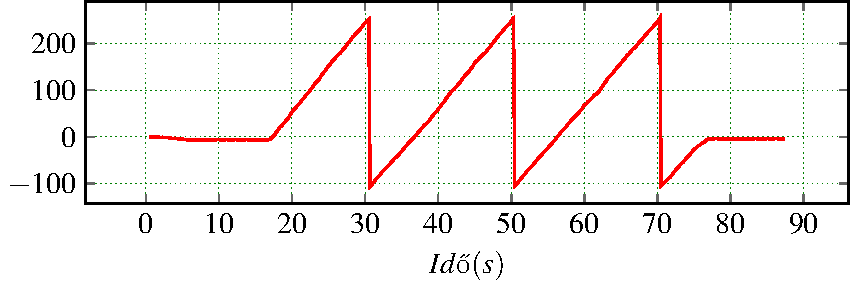
\includegraphics{tikz/Left_n50Right50c.pdf}
  \caption{$SSMR-4W$ típusú robot orientacioja, kereksebessegek BL=FL=-50 es a FR=BR= 50\degree/s}
\end{figure}


\begin{figure}[H]
  \label{fig:Left_n50Right50d}
  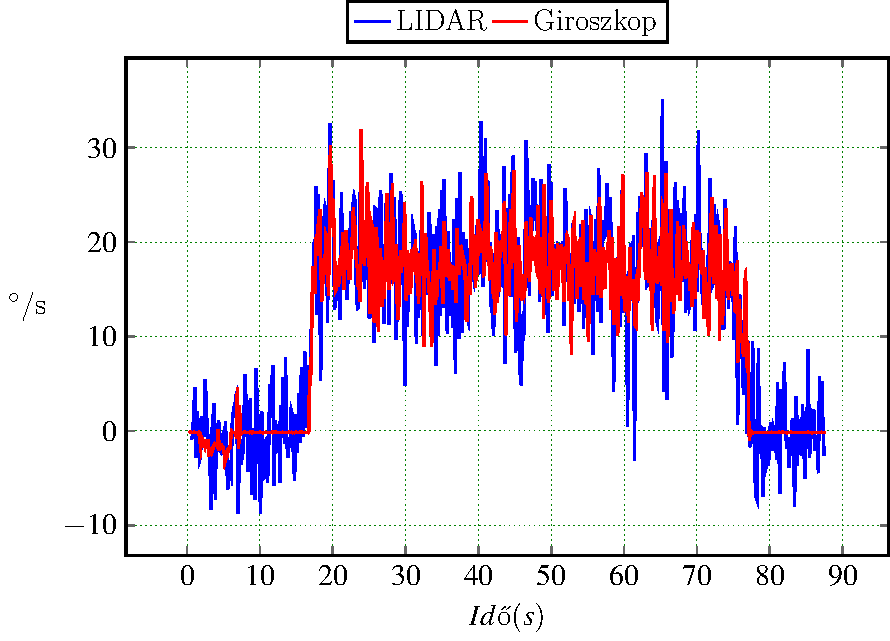
\includegraphics{tikz/Left_n50Right50d.pdf}
  \caption{$SSMR-4W$ típusú robot fordulasi szogsebessege, kereksebessegek BL=FL=-50 es a FR=BR= 50\degree/s}
\end{figure}











\subsection{Kavicsos talajon korpalyan mozgas}


\subsection{Kavicsos talajon korpalyan 50/15}
A \ref{fig:KorP0705a} megfigyelhető amint a robot kavicsos talajon differenciálisan fordul 80 másodpercen keresztül, ezalatt másfélszer körbefordul.

\renewcommand{\GlobalPath}{Meresek/Mozgasok/NormalMukodes/Korpalya_07_05_Kavicsos/}
\renewcommand{\secondImage}{*}

%kep a talajrol
%\input{Meresek/Mozgasok/KepekAFelszinrol.tex}

%1
%\input{Meresek/Mozgasok/FirstV1.tex}

\begin{figure}[H]
  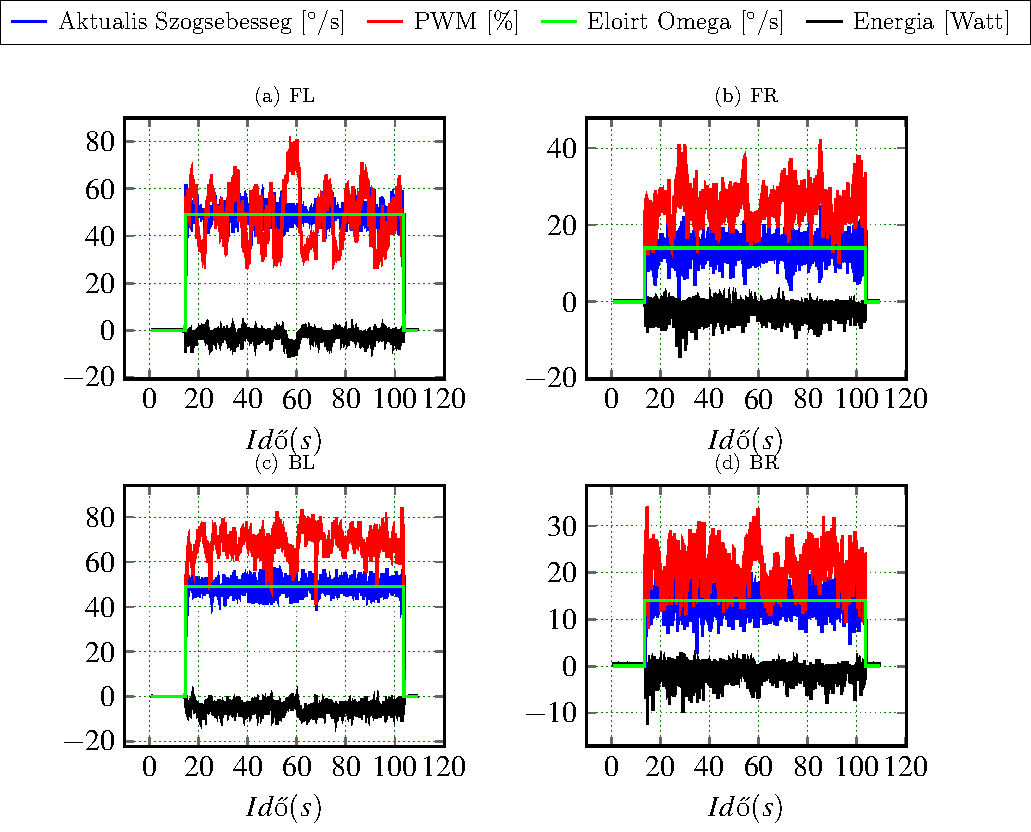
\includegraphics{tikz/KorP0705x.pdf}
  \caption{$SSMR-4W$ típusú robot mozgása, tengelyekre bontva, keréksebességek BL=FL=50\degree/s és a FR=BR=15\degree/s}
  \label{fig:KorP0705x}  
\end{figure}


\begin{figure}[H]
  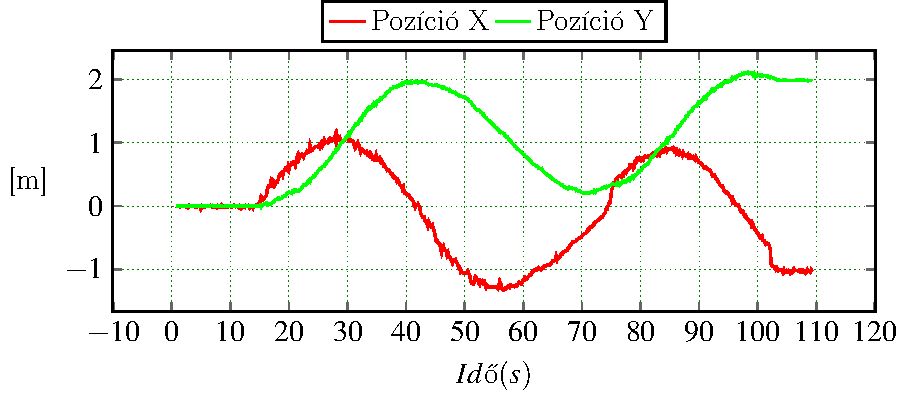
\includegraphics{tikz/KorP0705a.pdf}
  \caption{$SSMR-4W$ típusú robot mozgása, tengelyekre bontva, kerekszögsebességek BL=FL=50\degree/s és a FR=BR=15\degree/s}
  \label{fig:KorP0705a}  
\end{figure}


\begin{figure}[H]
  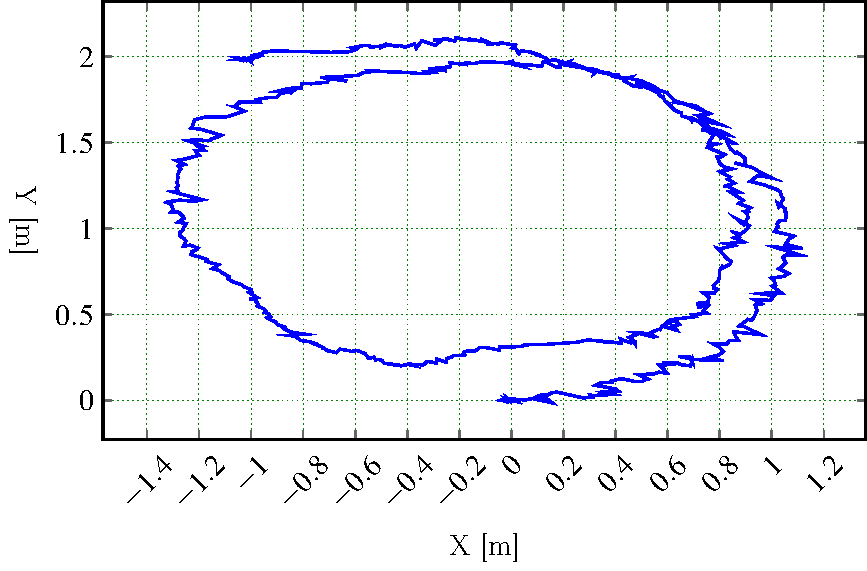
\includegraphics{tikz/KorP0705b.pdf}
  \caption{$SSMR-4W$ típusú robot altal leirt palya, kerekszögsebességek BL=FL=50\degree/s és a FR=BR=15\degree/s}
  \label{fig:KorP0705b}
\end{figure}

A körpalyán mozgás során a robot eltér a szabályos körtöl, és  látható a \ref{fig:KorP0705b} ábrán. A mérések nyilthurokan törének, nincs szabályzókör a pozicióra és a sebességkre.
A szögsebességet tekintve a robot 7\degree/s szögsebességet generál.


%\begin{figure}[H]
%  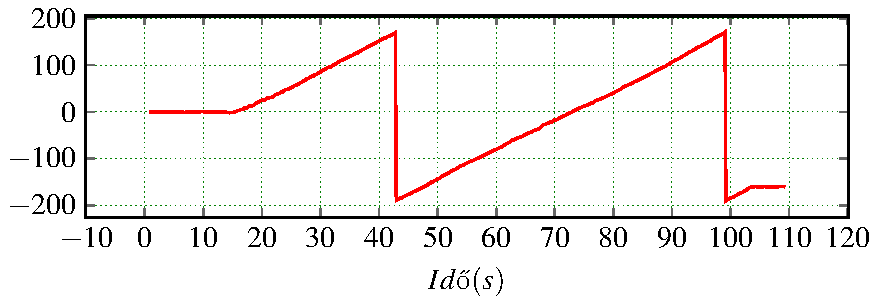
\includegraphics{tikz/KorP0705c.pdf}
%  \caption{$SSMR-4W$ típusú robot orientacioja, kerekszögsebességek %BL=FL=50\degree/s és a FR=BR=15\degree/s}
%  \label{fig:KorP0705c}
%\end{figure}


\begin{figure}[H]
\begin{center}
  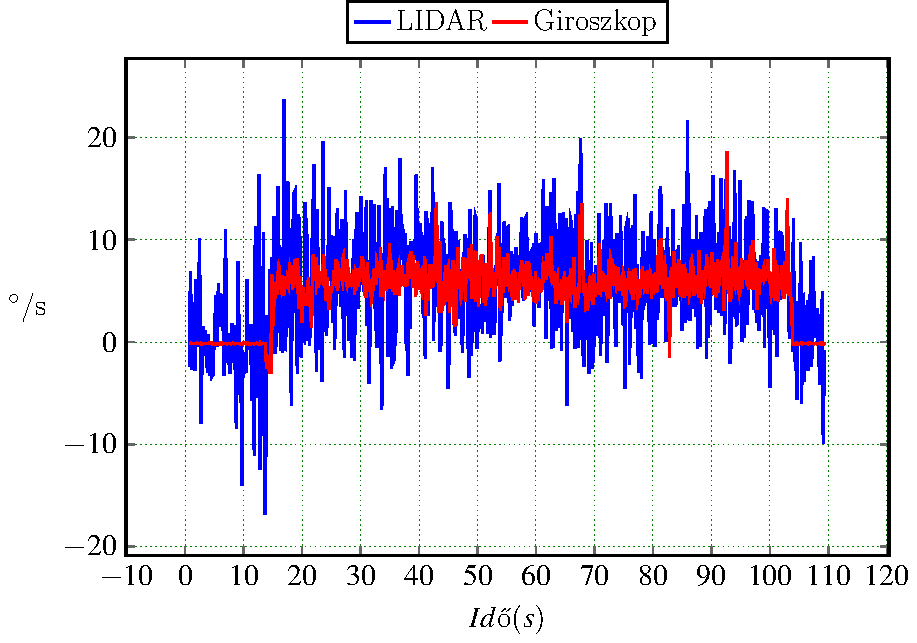
\includegraphics[scale=0.8]{tikz/KorP0705d.pdf}
\end{center}
  \caption{$SSMR-4W$ típusú robot fordulasi szögsebessége, kerekszögsebességek BL=FL=50\degree/s és a FR=BR=15\degree/s}
  \label{fig:KorP0705d}
\end{figure}


\begin{figure}[H]
\begin{center}
  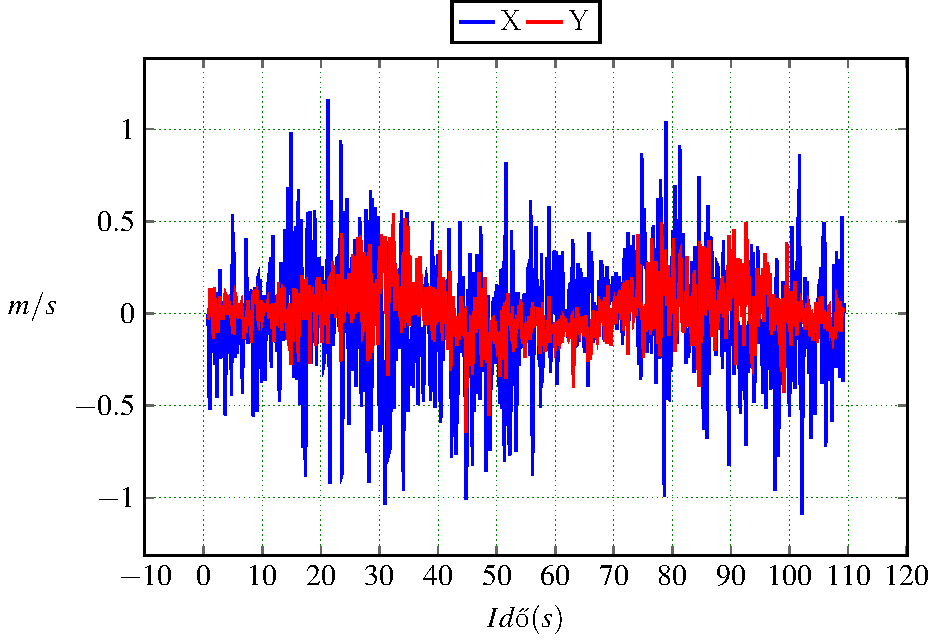
\includegraphics[scale=0.8]{tikz/KorP0705e.pdf}
\end{center}
  \caption{$SSMR-4W$ típusú robot egyenesvonalú sebességei, kerekszögsebességek BL=FL=50\degree/s és a FR=BR=15\degree/s}
  \label{fig:KorP0705e}
\end{figure}

A robot sebességét tekintve a \ref{fig:KorP0705e} látható hogy szinuszosan változuk a pozicióhoz hasonlóan,a robot kiss sebességü mozgása miatt a mérés zajos.
;
\subsection{Kavicsos talajon körpályán 50/25}

Az alábbi méréseknél 80-90s között a robot jobboldali kerekeit vezérlő H-híd túlmelegedése miatt a beléjük épített védelmi funkciónak köszönhetően leálltak így a jobboldali kerek leblokkoltak, így a mozgás pályája is megváltozott.


\renewcommand{\GlobalPath}{Meresek/Mozgasok/NormalMukodes/Korpalya_07_03_Kavicsos/}
\renewcommand{\secondImage}{*}

%kep a talajrol
%\input{Meresek/Mozgasok/KepekAFelszinrol.tex}

%1
%\input{Meresek/Mozgasok/FirstV1.tex}



\begin{figure}[H]
  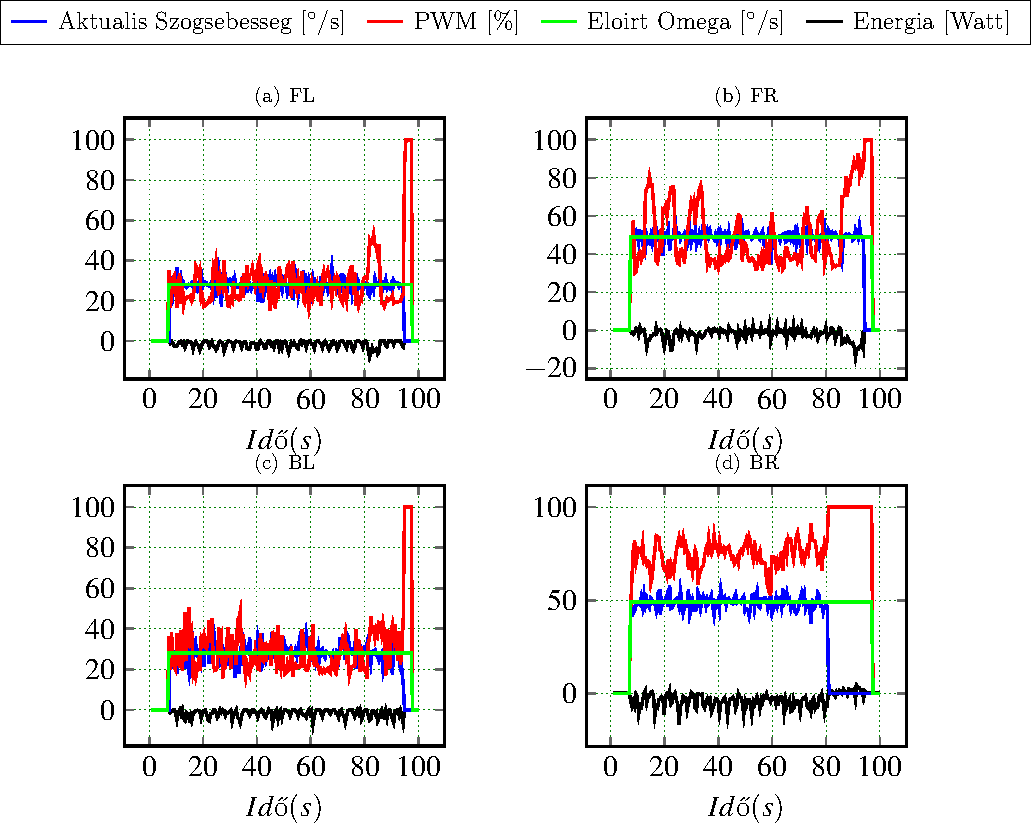
\includegraphics{tikz/KorP0703x.pdf}
  \caption{$SSMR-4W$ típusú robot motorvezérlő jelei, ha kerékszögsebességek BL=FL=25\degree/s és a FR=BR=50\degree/s}
  \label{fig:KorP0703x}
\end{figure}


\begin{figure}[H]
  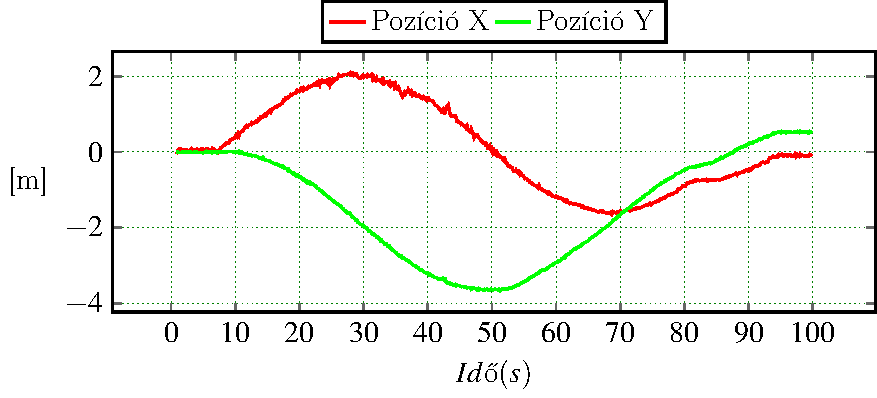
\includegraphics{tikz/KorP0703a.pdf}
  \caption{$SSMR-4W$ típusú robot mozgása, tengelyekre bontva, ha kerékszögsebességek BL=FL=25\degree/s és a FR=BR=50\degree/s }
  \label{fig:KorP0703a}
\end{figure}



\begin{figure}[H]
  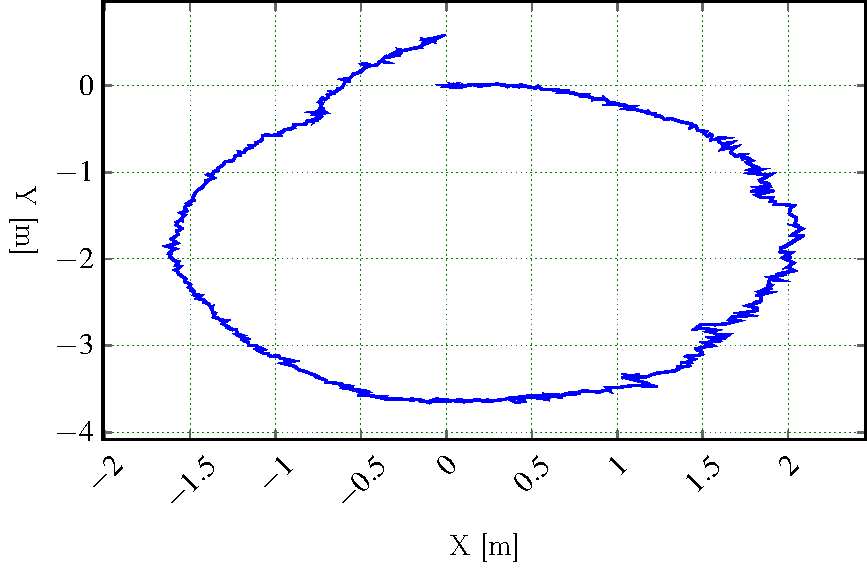
\includegraphics{tikz/KorP0703b.pdf}
  \caption{$SSMR-4W$ típusú robot által leírt pálya, ha kerékszögsebességek BL=FL=25\degree/s és a FR=BR=50\degree/s}
  \label{fig:KorP0703b}
\end{figure}


%\begin{figure}[H]
%  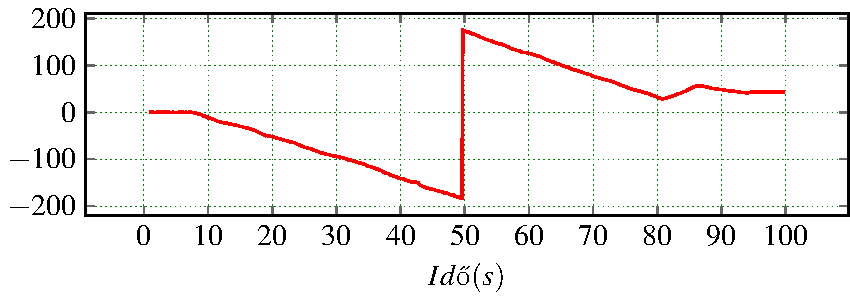
\includegraphics{tikz/KorP0703c.pdf}
%  \caption{$SSMR-4W$ típusú robot orientációja, ha kerékszögsebességek %BL=FL=25\degree/s és a FR=BR=50\degree/s}
%  \label{fig:KorP0703c}
%\end{figure}


\begin{figure}[H]
  \begin{center}
  	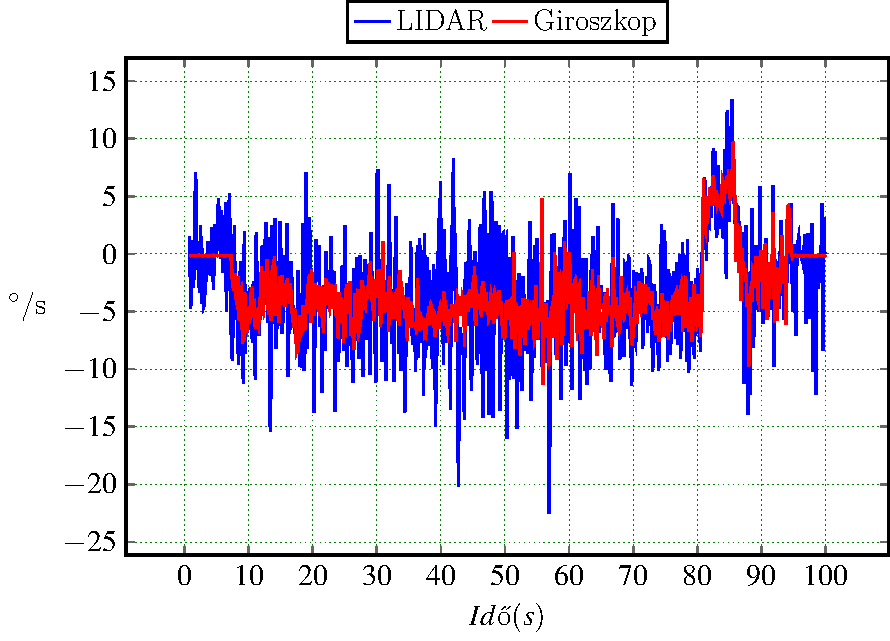
\includegraphics[scale=1]{tikz/KorP0703d.pdf}
  \end{center}
  \caption{$SSMR-4W$ típusú robot fordulási szögsebessége, ha kerékszögsebességek BL=FL=25\degree/s és a FR=BR=50\degree/s}
  \label{fig:KorP0703d}
\end{figure}

%\begin{figure}[H]
%  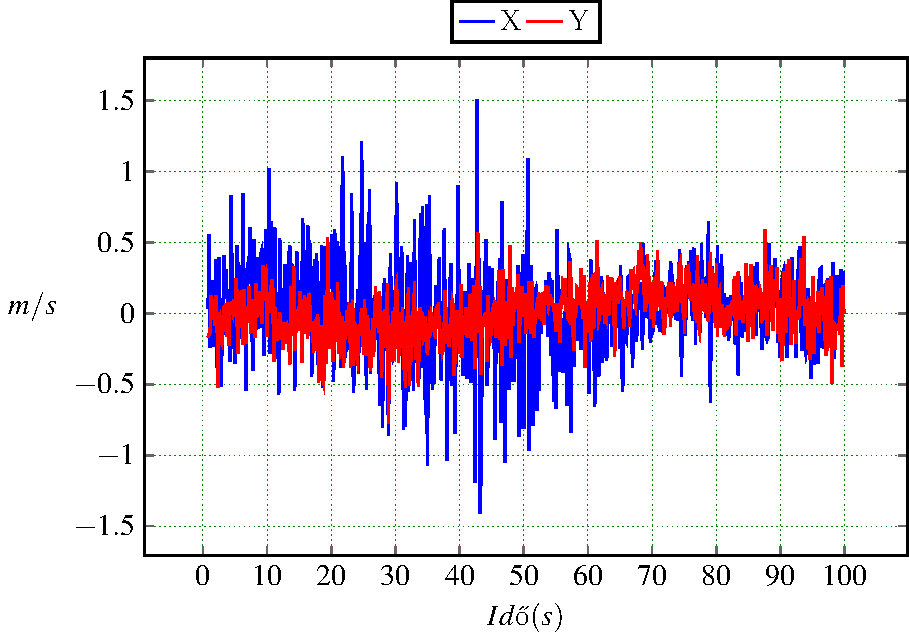
\includegraphics{tikz/KorP0703e.pdf}
%  \caption{$SSMR-4W$ típusú robot egyenesvonalu sebessegei, ha %kerékszögsebességek BL=FL=25\degree/s és a FR=BR=50\degree/s}
%  \label{fig:KorP0703e}
%\end{figure}


;

------------------------------------


\begin{figure}[H]
  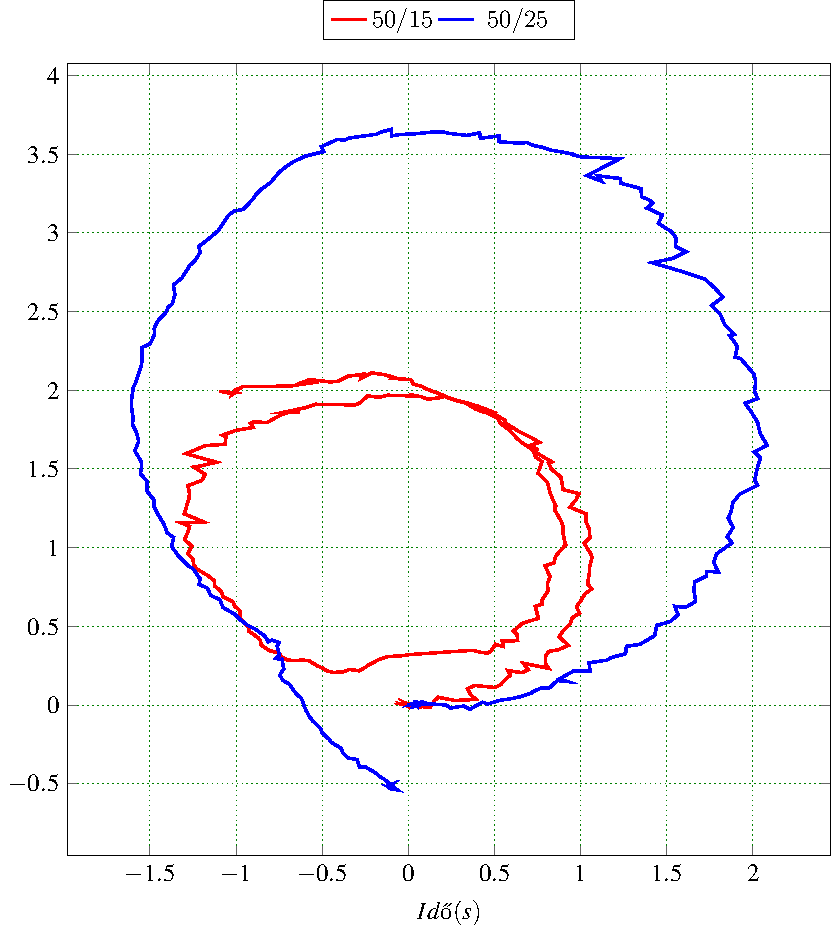
\includegraphics{tikz/KorpalyakKavicsos.pdf}
  \caption{Kulombozo korpalyak}
  \label{fig:KorpalyakKavicsos}  
\end{figure}





\renewcommand{\GlobalPath}{Meresek/Mozgasok/GyergyoFuvesUdvar/M1/}
\renewcommand{\plotRotSpeed}{o}
\renewcommand{\plotSpeed}{o}
%
\subsubsection{Talajon valo mozgas meresi eredmenyei}


\renewcommand{\AbraFelirat}{$SSMR-4W$ tipusu robot kereknyomoerok kerekenkeni változása a sulypont fuggvenyebenddd}

%kep a talajrol


\renewcommand{\sources}{}
\renewcommand{\captionn}{Kep a felszinrol}
\renewcommand{\figlabel}{figm}


\begin{kep}
    \begin{figure}[H]%
    \begin{center}
    
    \subfloat[label a]{
        {\includegraphics[width=9cm]{\mand{\GlobalPath}{talaj1.jpg}} }
        \label{fig:ex3-a}
    }%
    
    \ifthenelse{\equal{\secondImage}{*}}
    {}
    {
        \qquad
        \subfloat[label b]{{\includegraphics[width=9cm]{\mand{\GlobalPath}{talaj1.jpg}} }}%
    }
  
    \label{fig:example}%
    \end{center}
\end{figure}
\end{kep}

\renewcommand{\secondImage}{*}



%1
 %1
    \begin{figure}
    
        %-------------------------------------------------Joint Adatok---------------
        \begin{subfigure}{\textwidth}
            \begin{center}
        
            \input{\mand{\GlobalPath}{L.tex}}
            \pgfplotstableread{NodeLeft.dat}{\leftNode}

            
            \input{\mand{\GlobalPath}{R.tex}}
            \pgfplotstableread{NodeRight.dat}{\rightNode}

        
            \begin{tikzpicture}
            \pgfplotsset{every axis plot/.append style={very thick}}
            \setcaptionsubtype
            
            % megjelenites beallitasai
            
            \begin{groupplot}[%
                        ,group style={%
                            ,group name=my plots
                            ,group size=2 by 2
                            ,vertical sep=1.8cm,
                            ,horizontal sep = 2.4cm,
                            ,ylabels at=edge left
                        }
                        ,width=7cm
                        ,height=6cm
                        ,try min ticks=5
                        ,xlabel={\bfseries{\emph{\idoFelirat}}}
                        ,zlabel={\bfseries{\emph{kg}}}
                        %%ha kell y felirat az elso ketore
                        %,ylabel={\bfseries{\degree$/s$}}
                        %,ylabel style={rotate=-90}
                        %,xtick={0,10,...,60},
                        %,minor tick num=5
                        %,xtick distance=10
                        %,ytick distance=25
                        ,grid=major%both
                        ,every both grid/.style={gray, opacity=0.7},
                        view={0}{90},
                        legend columns=2,
                        %xmin=0,xmax=0.65,
                        %ymin=0,ymax=0.65,
                       % zmin=-5,zmax=60,
                        ]
            %% ide jonnek a adatok. 
            
            %ha kell felirat be kell teni a nextplot[] parameterei koze
            % \nextgroupplot[ylabel=\degree$/s$, ylabel style={rotate=-90},legend to name={CommonLegend},legend style={legend columns=2}]
            \nextgroupplot[]
                \addplot [color=green,each nth point={\nth}] table [header=true, x=Time, y=refOmegaA] {\leftNode};\label{plots:plot3}
                \addplot [color=black,each nth point={\nth}] table [header=true, x=Time, y=effortA] {\leftNode};\label{plots:plot4}
                \addplot [color=blue,each nth point={\nth}] table [header=true, x=Time, y=omegaA] {\leftNode}; \label{plots:plot1}
                \addplot [color=red,each nth point={\nth}] table [header=true, x=Time, y=pwmA] {\leftNode};\label{plots:plot2}
                \coordinate (top) at (rel axis cs:0,1);% coordinate at top of the first plot
            
            \nextgroupplot[]
                \addplot [color=green,each nth point={\nth}] table [header=true, x=Time, y=refOmegaA] {\rightNode};
                \addplot [color=black,each nth point={\nth}] table [header=true, x=Time, y=effortA] {\rightNode};
                \addplot [color=blue,each nth point={\nth}] table [header=true, x=Time, y=omegaA] {\rightNode};
                \addplot [color=red,each nth point={\nth}] table [header=true, x=Time, y=pwmA] {\rightNode};
                    
            \nextgroupplot[]
                \addplot [color=green,each nth point={\nth}] table [header=true, x=Time, y=refOmegaB] {\leftNode};
                \addplot [color=black,each nth point={\nth}] table [header=true, x=Time, y=effortB] {\leftNode};
                \addplot [color=blue,each nth point={\nth}] table [header=true, x=Time, y=omegaB] {\leftNode};
                \addplot [color=red,each nth point={\nth}] table [header=true, x=Time, y=pwmB] {\leftNode};
                   
            \nextgroupplot[]
                \addplot [color=green,each nth point={\nth}] table [header=true, x=Time, y=refOmegaB] {\rightNode};
                \addplot [color=black,each nth point={\nth}] table [header=true, x=Time, y=effortB] {\rightNode};
                \addplot [color=blue,each nth point={\nth}] table [header=true, x=Time, y=omegaB] {\rightNode};
                \addplot [color=red,each nth point={\nth}] table [header=true, x=Time, y=pwmB] {\rightNode};
                \coordinate (bot) at (rel axis cs:1,0);% coordinate at bottom of the last plot
            \end{groupplot}
            
            %\path [nodes={anchor=south,rotate=90,font=\large\bfseries,midway}]
            %  (my plots c1r1.outer north west)--(my plots c1r2.outer south west)
            %    node {Testing of Parameters 1}
            %  (my plots c2r1.outer north west)--(my plots c2r2.outer south west)
            %    node {Testing of Parameters 2};
            
            % legend
            \node[text width=.5\linewidth,align=center,anchor=south] at (my plots c1r1.north) {\caption[]{FL\label{subplot:one}}};
            \node[text width=.5\linewidth,align=center,anchor=south] at (my plots c2r1.north) {\caption[]{FR\label{subplot:two}}};
            \node[text width=.5\linewidth,align=center,anchor=south] at (my plots c1r2.north) {\caption[]{BL\label{subplot:three}}};
            \node[text width=.5\linewidth,align=center,anchor=south] at (my plots c2r2.north) {\caption[]{BR\label{subplot:four}}};
            
            %\path (top-|current bounding box.west)-- 
            %      node[anchor=south,rotate=90] {throughput} 
            %      (bot-|current bounding box.west);
            % legend
            \path (top|-current bounding box.north)--
                  coordinate(legendpos)
                  (bot|-current bounding box.north);
            \matrix[
                matrix of nodes,
                anchor=south,
                draw,
                inner sep=0.2em,
                draw
              ]at([yshift=1ex]legendpos)
              {
                \ref{plots:plot1}& Aktualis Szogsebesseg [\degree$/s$]&[5pt]
                \ref{plots:plot2}& PWM [$\%$] &[5pt]
                \ref{plots:plot3}& Eloirt Omega [\degree$/s]$
                \ref{plots:plot4}& Energia $[Watt]$ &[5pt]\\
            };
           % \centering
            \end{tikzpicture}
            \end{center}
        \end{subfigure}
        
        \iffalse
        %-------------------------------------------------Power Adatok---------------
        \newline
        \begin{subfigure}{\textwidth}
        \begin{center}
        \input{\mand{\GlobalPath}{Power.tex}}
        \pgfplotstableread{Power.dat}{\power}
        
        
        \begin{tikzpicture}
        \pgfplotsset{every axis plot/.append style={very thick}}
        \setcaptionsubtype
        
        % megjelenites beallitasai
        
        \begin{groupplot}[%
                    ,group style={%
                        ,group name=my plots
                        ,group size=1 by 1
                        ,vertical sep=2cm,
                        ,horizontal sep = 0cm,
                        ,ylabels at=edge left
                    }
                    ,width=14.5cm
                    ,height=6cm
                    ,try min ticks=5
                    ,xlabel={\bfseries{\emph{\idoFelirat}}}
                    %,ylabel={\bfseries{\emph{A}}}
                    %,zlabel={\bfseries{\emph{kg}}}
                    ,grid=both
                    ,every both grid/.style={gray, opacity=0.5}
                    ,view={0}{90},
                    %,xtick distance=10
                    %,minor tick num=5
                    %,ytick distance=5
                    %xmin=0,xmax=0.65,
                    %ymin=0,ymax=0.65,
                    %zmin=-5,zmax=60,
                    ]
        %% ide jonnek a adatok.            
                    
        \nextgroupplot[ylabel=\emph{}, ylabel style={rotate=-90}]
         \addplot [color=red,each nth point={\nth}] table [header=true, x=Time, y=voltage] {\power};\label{plots:plot11}
         \addplot [color=green,each nth point={\nth}] table [header=true, x=Time, y=current]{\power};\label{plots:plot12}
         \addplot [color=black,each nth point={\nth}] table [header=true, x=Time, y=power] {\power};\label{plots:plot13}
        \end{groupplot}
        
        %\path [nodes={anchor=south,rotate=90,font=\large\bfseries,midway}]
        %  (my plots c1r1.outer north west)--(my plots c1r2.outer south west)
        %    node {Testing of Parameters 1}
        %  (my plots c2r1.outer north west)--(my plots c2r2.outer south west)
        %    node {Testing of Parameters 2};
        
        % legend
        \node[text width=.5\linewidth,align=center,anchor=south] at (my plots c1r1.north) {\caption[]{Energia Fogyasztas\label{subplot:one}}};
        
        %\path (top-|current bounding box.west)-- 
            %      node[anchor=south,rotate=90] {throughput} 
            %      (bot-|current bounding box.west);
            % legend
            \path (top|-current bounding box.north)--
                  coordinate(legendpos)
                  (bot|-current bounding box.north);
            \matrix[
                matrix of nodes,
                anchor=south,
                draw,
                inner sep=0.2em,
                draw
              ]at([yshift=1ex]legendpos)
              {
                \ref{plots:plot11}&  Akumlator Feszultsege [V]&[5pt]
                \ref{plots:plot12}& Akkumlator Arama [A] &[5pt]
                \ref{plots:plot13}& Teljesitmeny [W] \\
            };
        
        %\centering
        \end{tikzpicture}
        \end{center}
        \end{subfigure}
        % Caption
        %\caption[]{$SSMR-4W$ tipusu robot kereknyomoerok kerekenkeni változása a sulypont fuggvenyeben}\label{abserror}
        \fi
    \end{figure}

%2
    %2
    \begin{figure}[H]
        %\ContinuedFloat
        %-------------------------------------------------Pozicio X es Y Adatok---------------
       % \newline
        \begin{subfigure}{\textwidth}
        \begin{center}
           \input{\mand{\GlobalPath}{Pos.tex}}
            \pgfplotstableread{PositionOrientation.dat}{\pos}
            \centering
            \begin{tikzpicture}
            \pgfplotsset{every axis plot/.append style={very thick}}
            \setcaptionsubtype
            
            % megjelenites beallitasai
            
            \begin{groupplot}[%
                        ,group style={%
                            ,group name=my plots
                            ,group size=1 by 1
                            ,vertical sep=2cm,
                            ,horizontal sep = 0cm,
                            ,ylabels at=edge left
                        }
                        ,width=14.5cm
                        ,height=6cm
                        ,try min ticks=5
                        ,xlabel={\bfseries{\emph{\idoFelirat}}}
                        %,ylabel={\bfseries{\emph{A}}}
                        %,zlabel={\bfseries{\emph{kg}}}
                        ,grid=both
                        ,every both grid/.style={gray, opacity=0.5}
                        ,view={0}{90},
                        %,xtick distance=10
                        %,ytick distance=0.4
                        %,minor tick num=5
                        %xmin=0,xmax=0.65,
                        %ymin=0,ymax=0.65,
                        %zmin=-5,zmax=60,
                        ]
            %% ide jonnek a adatok.            
                        
            \nextgroupplot[ylabel=\emph{m}, ylabel style={rotate=-90}]
             \addplot [color=red,each nth point={\nth}] table [header=true, x=Time, y=poseX] {\pos};\label{plots:plot21}
             %\addlegendentry{Pozíció X [m]} 
             \addplot [color=green,each nth point={\nth}] table [header=true, x=Time, y=poseY]{\pos};\label{plots:plot22}                            %\addlegendentry{Pozíció Y [m]} 
            \end{groupplot}
            
            %\path [nodes={anchor=south,rotate=90,font=\large\bfseries,midway}]
            %  (my plots c1r1.outer north west)--(my plots c1r2.outer south west)
            %    node {Testing of Parameters 1}
            %  (my plots c2r1.outer north west)--(my plots c2r2.outer south west)
            %    node {Testing of Parameters 2};
            
            % legend
            \node[text width=.5\linewidth,align=center,anchor=south] at (my plots c1r1.north) {\caption[]{Robot Pozíció Tengelyekre           \label{subplot:\figlabela}}};
            
            %\path (top-|current bounding box.west)-- 
                %      node[anchor=south,rotate=90] {throughput} 
                %      (bot-|current bounding box.west);
                % legend
                \path (top|-current bounding box.north)--
                      coordinate(legendpos)
                      (bot|-current bounding box.north);
                \matrix[
                    matrix of nodes,
                    anchor=south,
                    draw,
                    inner sep=0.2em,
                    draw
                  ]at([yshift=1ex]legendpos)
                  {
                    \ref{plots:plot21}&Pozíció X [m] &[5pt]
                    \ref{plots:plot22}&Pozíció Y [m] &[5pt]\\
                };
            
            %\centering
            \end{tikzpicture}
            \end{center}
        \end{subfigure}
        
        %-------------------------------------------------Palya Adatok---------------
      %  \newline
        \begin{subfigure}{\textwidth}
           \begin{center}
            \input{\mand{\GlobalPath}{/Pos.tex}}
            \pgfplotstableread{PositionOrientation.dat}{\position}
            
            \begin{tikzpicture}
                \pgfplotsset{every axis plot/.append style={very thick}}
                \setcaptionsubtype
            
                % megjelenites beallitasai
            
                \begin{groupplot}[%
                        ,group style={%
                            ,group name=my plots
                            ,group size=1 by 1
                            ,vertical sep=2cm,
                            ,horizontal sep = 0cm,
                            ,ylabels at=edge left
                        }
                        ,width=14.5cm
                        ,height=9cm
                        %,try min ticks=5
                        ,xlabel={\bfseries{\emph{m}}}
                        ,ylabel={\bfseries{\emph{m}}}
                        ,zlabel={\bfseries{\emph{\idoFelirat}}}
                        ,grid=both
                        ,every both grid/.style={gray, opacity=0.5}
                        ,view={45}{45}
                        %,xtick distance=0.25
                        %,ytick distance=0.25
                        %,minor tick num=5
                        ,xticklabel style={rotate=45},
                        ,ylabel style={rotate=-90}
                        %xmin=0,xmax=0.65,
                        %ymin=0,ymax=0.65,
                       % zmin=-5,zmax=60,
                        ]
                    %% ide jonnek a adatok.            
                                
                    %\nextgroupplot[ylabel=\emph{A}, ylabel style={rotate=-90}]
                    \nextgroupplot[]
                           % \addplot3 []  table [header=true, x=poseX, y=poseY, z=Time] {\position};
                           
                            \addplot [color=blue,each nth point={\nth}] table [header=true, x=poseX, y=poseY] {\position};
                            
                            %\addplot [color=blue] table [header=true, x=poseX, y=poseY] {\position};
                         %%   \addplot[red,quiver={u=u,v=v}] table [header=true, x=poseX, y=poseY, u=poseX, v=poseY] {\position};
        
        
        
        
            \end{groupplot}
            
                %\path [nodes={anchor=south,rotate=90,font=\large\bfseries,midway}]
                %  (my plots c1r1.outer north west)--(my plots c1r2.outer south west)
                %    node {Testing of Parameters 1}
                %  (my plots c2r1.outer north west)--(my plots c2r2.outer south west)
                %    node {Testing of Parameters 2};
                
                % legend
                \node[text width=.5\linewidth,align=center,anchor=south] at (my plots c1r1.north) {\caption[]{Robot Által Leirt Pálya     \label{subplot:\figlabelb}}};
                
                %\centering
            \end{tikzpicture}
            \end{center}
    \end{subfigure}
        
        %-------------------------------------------------Orientacio Adatok---------------
       % \newline
        \begin{subfigure}{\textwidth}
        \begin{center}
        \input{\mand{\GlobalPath}{Pos.tex}}
        \pgfplotstableread{PositionOrientation.dat}{\pos}
        
        \begin{tikzpicture}
        \pgfplotsset{every axis plot/.append style={very thick}}
        \setcaptionsubtype
        
        % megjelenites beallitasai
        
        \begin{groupplot}[%
                    ,group style={%
                        ,group name=my plots
                        ,group size=1 by 1
                        ,vertical sep=2cm,
                        ,horizontal sep = 0cm,
                        ,ylabels at=edge left
                    }
                    ,width=14.5cm
                    ,height=5cm
                    ,try min ticks=5
                    ,xlabel={\bfseries{\emph{\idoFelirat}}}
                    %,ylabel={\bfseries{\emph{A}}}
                    %,zlabel={\bfseries{\emph{kg}}}
                    ,grid=both
                    ,every both grid/.style={gray, opacity=0.5}
                    ,view={0}{90},
                    %,xtick distance=10
                    %,ytick distance=20
                    %,minor tick num=5
                    %xmin=0,xmax=0.65,
                    %ymin=0,ymax=0.65,
                    %zmin=-5,zmax=60,
                    ]
        %% ide jonnek a adatok.            
                    
        \nextgroupplot[ylabel=\emph{$[\degree]$}], ylabel style={rotate=-90}]
        \addplot [color=red,each nth point={\nth}] table [header=true, x=Time, y=orZ] {\pos};\label{plots:plot41}
        \end{groupplot}
        
        %\path [nodes={anchor=south,rotate=90,font=\large\bfseries,midway}]
        %  (my plots c1r1.outer north west)--(my plots c1r2.outer south west)
        %    node {Testing of Parameters 1}
        %  (my plots c2r1.outer north west)--(my plots c2r2.outer south west)
        %    node {Testing of Parameters 2};
        
        % legend
        \node[text width=.5\linewidth,align=center,anchor=south] at (my plots c1r1.north) {\caption[]{Orientáció \label{subplot:\figlabelc}}};
        
        
       % \centering
        \end{tikzpicture}
        \end{center}
        \end{subfigure}
    
        
        % Caption
        \ifthenelse{\equal{\captionn}{*}}
        {}
        {\captionof{figure}{\captionn}}
        \renewcommand{\captionn}{*}
        \label{subplot:\figlabel}
       
    \end{figure}
    
        \renewcommand{\figlabel}{*}
        \renewcommand{\figlabela}{*}
        \renewcommand{\figlabelb}{*}
        \renewcommand{\figlabelc}{*}

%3
%    %3
    \begin{figure}
        %\ContinuedFloat
        \input{\mand{\GlobalPath}{Pos.tex}}
        \ifthenelse{\equal{\plotSpeed}{*}}
        { }
        {
        \newline
        \begin{subfigure}{\textwidth}
            \begin{center}

            \pgfplotstableread{PositionOrientation.dat}{\position}
            
            %-------------------------------------------------Sebesseg Adatok---------------
            \begin{tikzpicture}
                \pgfplotsset{every axis plot/.append style={very thick}}
                \setcaptionsubtype
            
                % megjelenites beallitasai
            
                \begin{groupplot}[%
                        ,group style={%
                            ,group name=my plots
                            ,group size=1 by 1
                            ,vertical sep=2cm,
                            ,horizontal sep = 0cm,
                            ,ylabels at=edge left
                        }
                        ,width=14.5cm
                        ,height=10cm
                        ,try min ticks=5
                        ,ylabel={\bfseries{\emph{$m/s$}}}
                        ,xlabel={\bfseries{\emph{\idoFelirat}}}
                        %,zlabel={\bfseries{\emph{m}}}
                        ,grid=both
                        ,every both grid/.style={gray, opacity=0.5}
                        ,view={0}{90}
                        %,xtick distance=10
                        %,ytick distance=0.1
                        ,ylabel style={rotate=-90}
                        %xmin=0,xmax=0.65,
                        %ymin=0,ymax=0.65,
                       % zmin=-5,zmax=60,
                        ]
                    %% ide jonnek a adatok.            
                                
                    %\nextgroupplot[ylabel=\emph{A}, ylabel style={rotate=-90}]
                    \nextgroupplot[]
                            \addplot [color=blue,each nth point={\nth}] table [header=true, x=Time, y=speedX] {\position}; \label{plots:plot51}
                            \addplot [color=red,each nth point={\nth}] table [header=true, x=Time, y=speedY] {\position}; \label{plots:plot52}
                         %%   \addplot[red,quiver={u=u,v=v}] table [header=true, x=poseX, y=poseY, u=poseX, v=poseY] {\position};
        
        
        
        
            \end{groupplot}
            
                %\path [nodes={anchor=south,rotate=90,font=\large\bfseries,midway}]
                %  (my plots c1r1.outer north west)--(my plots c1r2.outer south west)
                %    node {Testing of Parameters 1}
                %  (my plots c2r1.outer north west)--(my plots c2r2.outer south west)
                %    node {Testing of Parameters 2};
                
                % legend
                \node[text width=.5\linewidth,align=center,anchor=south] at (my plots c1r1.north) {\caption[]{Robot Sebessége a Globális Koordináta Rendszerben
               \label{subplot:\figlabela}}};
                
                      %\path (top-|current bounding box.west)-- 
                %      node[anchor=south,rotate=90] {throughput} 
                %      (bot-|current bounding box.west);
                % legend
                \path (top|-current bounding box.north)--
                      coordinate(legendpos)
                      (bot|-current bounding box.north);
                \matrix[
                    matrix of nodes,
                    anchor=south,
                    draw,
                    inner sep=0.2em,
                    draw
                  ]at([yshift=1ex]legendpos)
                  {
                    \ref{plots:plot51}& Sebesség X &[5pt] 
                    \ref{plots:plot52}& Sebesség Y &[5pt]\\
                  };
                
                %\centering
            \end{tikzpicture}
            \end{center}
        \end{subfigure}
        }
        
        \ifthenelse{\equal{\plotRotSpeed}{*}}
        { }
        { 
        %-------------------------------------------------Fordulasi Sebesseg Adatok---------------
        \newline
        \input{\mand { \GlobalPath}{Pos.tex}}
        \pgfplotstableread{PositionOrientation.dat}{\position}
        
        \input{\mand{\GlobalPath}{ImuA.tex}}
        \pgfplotstableread{ImuA.dat}{\imua}
        
        \begin{subfigure}{\textwidth}
            \begin{center}

            
            \begin{tikzpicture}
                \pgfplotsset{every axis plot/.append style={very thick}}
                \setcaptionsubtype
            
                % megjelenites beallitasai
            
                \begin{groupplot}[%
                        ,group style={%
                            ,group name=my plots
                            ,group size=1 by 1
                            ,vertical sep=2cm,
                            ,horizontal sep = 0cm,
                            ,ylabels at=edge left
                        }
                        ,width=14.5cm
                        ,height=10cm
                        ,try min ticks=5
                        ,ylabel={\bfseries{\emph{\degree/s}}}
                        ,xlabel={\bfseries{\emph{\idoFelirat}}}
                        %,zlabel={\bfseries{\emph{m}}}
                        ,grid=both
                        ,every both grid/.style={gray, opacity=0.5}
                        ,view={0}{90}
                        %,xtick distance=10
                        %,ytick distance=10
                        ,ylabel style={rotate=-90}
                        %xmin=0,xmax=0.65,
                        %ymin=0,ymax=0.65,
                       % zmin=-5,zmax=60,
                        ]
                    %% ide jonnek a adatok.            
                                
                    %\nextgroupplot[ylabel=\emph{A}, ylabel style={rotate=-90}]
                    \nextgroupplot[]
                            \addplot [color=blue,each nth point={\nth}] table [header=true, x=Time, y=omegaZ] {\position}; \label{plots:plot61}
                            \addplot [color=red,each nth point={\nth}] table [header=true, x=Time, y expr=\thisrow{gZ}*-1] {\imua}; \label{plots:plot62}
                         %%   \addplot[red,quiver={u=u,v=v}] table [header=true, x=poseX, y=poseY, u=poseX, v=poseY] {\position};
        
        
        
        
            \end{groupplot}
            
                %\path [nodes={anchor=south,rotate=90,font=\large\bfseries,midway}]
                %  (my plots c1r1.outer north west)--(my plots c1r2.outer south west)
                %    node {Testing of Parameters 1}
                %  (my plots c2r1.outer north west)--(my plots c2r2.outer south west)
                %    node {Testing of Parameters 2};
                
                % legend
                \node[text width=.5\linewidth,align=center,anchor=south] at (my plots c1r1.north) {\caption[]{Robot Forgási Sebessége 
                \label{subplot:\figlabelb}}};
                
                        %\path (top-|current bounding box.west)-- 
                %      node[anchor=south,rotate=90] {throughput} 
                %      (bot-|current bounding box.west);
                % legend
                \path (top|-current bounding box.north)--
                      coordinate(legendpos)
                      (bot|-current bounding box.north);
                \matrix[
                    matrix of nodes,
                    anchor=south,
                    draw,
                    inner sep=0.2em,
                    draw
                  ]at([yshift=1ex]legendpos)
                  {
                    \ref{plots:plot61}& LIDAR  &[5pt] 
                    \ref{plots:plot62}& Giroszkop  &[5pt]\\
                };
                
               % \centering
            \end{tikzpicture}
            \end{center}
            
        \end{subfigure}
        }
        
        \renewcommand{\figlabela}{*}
        \renewcommand{\figlabelb}{*}
        
        % Caption
        \ifthenelse{\equal{\captionn}{*}}
        {}
        {\captionof{figure}{\captionn}}
        \renewcommand{\captionn}{*}

    
    \end{figure}

%Statistic
\DTLsetseparator{ = }% Set the separator between the columns. Could be
% anything you like. Whitespaces are not trimmed, so you have to set
%them as part of the separator.

\input{\mand{\GlobalPath}{Statistic.tex}}

        %\input{\mand{\GlobalPath}{Pos.tex}}
        %\pgfplotstableread{PositionOrientation.dat}{\pos}

\DTLdeletedb{mydataStat}
\DTLloaddb[noheader, keys={thekey,thevalue}]{mydataStat}{statistic.dat}
% Loads mydata.dat with column headers 'thekey' and 'thevalue'

\renewcommand{\missingcommand}[1]{\DTLfetch{mydataStat}{thekey}{#1}{thevalue}}

\begin{table}[H]
\begin{center}
    \begin{tabular}{llll}
        \hline
        Tulajdonság          & Node  & érték                                & Mértékegység                      \\ \hline
        Ossz sebesseg hiba   & FL & \missingcommand{SumErrorSpeedFL}        &   $[\degree/s]$                   \\
                             & BL & \missingcommand{SumErrorSpeedBL}        &   $[\degree/s]$                   \\
                             & FR & \missingcommand{SumErrorSpeedFR}        &   $[\degree/s]$                   \\
                             & BR & \missingcommand{SumErrorSpeedBR}        &   $[\degree/s]$                   \\
        Energia  fogyasztasa & FL & \missingcommand{PowerConsuptionFL}      &   $[W]$                           \\
                             & BL & \missingcommand{PowerConsuptionBL}      &   $[W]$                           \\
                             & FR & \missingcommand{PowerConsuptionFR}      &   $[W]$                           \\
                             & BR & \missingcommand{PowerConsuptionBR}      &   $[W]$                           \\
        Sulypont X           &    & \missingcommand{SulyPontX}              &   $[m]$                           \\
        Sulypont Y           &    & \missingcommand{SulyPontY}              &   $[m]$                           \\
        Ossz fordulas        &    & \missingcommand{Elfordulas}           &   $[\degree]$                     \\
        Megtett ut           &    & \missingcommand{Elmozdulas}              &   $[m]$                           \\
        Max Sebesseg         &    & \missingcommand{MaxSebesseg}            &   $[m\s]$                         \\
        Max ford Sebesseg    &    & \missingcommand{MaxFordulasiSebesseg}   &   $[\degree/s]$                   \\
    \end{tabular}
    \end{center}
\end{table}

%Imu
%   
    
    \begin{figure}[H]
        %\ContinuedFloat
        
            \tikzsetnextfilename{\figlabel}   
    
            \centering
             \input{\mand{\GlobalPath}{ImuA.tex}}
            \pgfplotstableread{ImuA.dat}{\imua}
            
            
             \begin{tikzpicture}
    
        \pgfplotsset{every axis plot/.append style={very thick}}
        \pgfplotsset{every axis legend/.append style={
        at={(0.5,1.03)},
        anchor=south}}
        
        \begin{axis}[
                ,width=14.5cm
                ,height=10cm
                ,try min ticks=5
                ,xlabel={\bfseries{\emph{\idoFelirat}}}
                ,ylabel={\bfseries{\emph{$m/{s^2}$}}}
                %,zlabel={\bfseries{\emph{kg}}}
                ,grid=both
                ,every both grid/.style={gray, opacity=0.5}
                ,view={0}{90},
                %,xtick distance=10
                %,ytick distance=20
                %,minor tick num=5
                %xmin=0,xmax=0.65,
                %ymin=0,ymax=0.65,
                %zmin=-5,zmax=60,
                ,legend columns=-1
              ]
              
               \addplot [color=red,each nth point={\nth}] table [header=true, x=Time, y expr=\thisrow{aX}] {\imua}; \addlegendentry {aX}
                            \addplot [color=blue,each nth point={\nth}] table [header=true, x=Time, y expr=\thisrow{aY}] {\imua}; \addlegendentry {aY}
                            \addplot [color=green,each nth point={\nth}] table [header=true, x=Time, y expr=\thisrow{aZ}] {\imua}; \addlegendentry {aZ}
            %\legend{\bfseries{\emph{Pozíció X}},\bfseries{\emph{Pozíció Y}}}
         
         \end{axis}
    \end{tikzpicture}
    
    \end{figure}





\renewcommand{\GlobalPath}{Meresek/Mozgasok/M6/}
%
\subsubsection{Talajon valo mozgas meresi eredmenyei}


\renewcommand{\AbraFelirat}{$SSMR-4W$ tipusu robot kereknyomoerok kerekenkeni változása a sulypont fuggvenyebenddd}

%kep a talajrol


\renewcommand{\sources}{}
\renewcommand{\captionn}{Kep a felszinrol}
\renewcommand{\figlabel}{figm}


\begin{kep}
    \begin{figure}[H]%
    \begin{center}
    
    \subfloat[label a]{
        {\includegraphics[width=9cm]{\mand{\GlobalPath}{talaj1.jpg}} }
        \label{fig:ex3-a}
    }%
    
    \ifthenelse{\equal{\secondImage}{*}}
    {}
    {
        \qquad
        \subfloat[label b]{{\includegraphics[width=9cm]{\mand{\GlobalPath}{talaj1.jpg}} }}%
    }
  
    \label{fig:example}%
    \end{center}
\end{figure}
\end{kep}

\renewcommand{\secondImage}{*}



%1
 %1
    \begin{figure}
    
        %-------------------------------------------------Joint Adatok---------------
        \begin{subfigure}{\textwidth}
            \begin{center}
        
            \input{\mand{\GlobalPath}{L.tex}}
            \pgfplotstableread{NodeLeft.dat}{\leftNode}

            
            \input{\mand{\GlobalPath}{R.tex}}
            \pgfplotstableread{NodeRight.dat}{\rightNode}

        
            \begin{tikzpicture}
            \pgfplotsset{every axis plot/.append style={very thick}}
            \setcaptionsubtype
            
            % megjelenites beallitasai
            
            \begin{groupplot}[%
                        ,group style={%
                            ,group name=my plots
                            ,group size=2 by 2
                            ,vertical sep=1.8cm,
                            ,horizontal sep = 2.4cm,
                            ,ylabels at=edge left
                        }
                        ,width=7cm
                        ,height=6cm
                        ,try min ticks=5
                        ,xlabel={\bfseries{\emph{\idoFelirat}}}
                        ,zlabel={\bfseries{\emph{kg}}}
                        %%ha kell y felirat az elso ketore
                        %,ylabel={\bfseries{\degree$/s$}}
                        %,ylabel style={rotate=-90}
                        %,xtick={0,10,...,60},
                        %,minor tick num=5
                        %,xtick distance=10
                        %,ytick distance=25
                        ,grid=major%both
                        ,every both grid/.style={gray, opacity=0.7},
                        view={0}{90},
                        legend columns=2,
                        %xmin=0,xmax=0.65,
                        %ymin=0,ymax=0.65,
                       % zmin=-5,zmax=60,
                        ]
            %% ide jonnek a adatok. 
            
            %ha kell felirat be kell teni a nextplot[] parameterei koze
            % \nextgroupplot[ylabel=\degree$/s$, ylabel style={rotate=-90},legend to name={CommonLegend},legend style={legend columns=2}]
            \nextgroupplot[]
                \addplot [color=green,each nth point={\nth}] table [header=true, x=Time, y=refOmegaA] {\leftNode};\label{plots:plot3}
                \addplot [color=black,each nth point={\nth}] table [header=true, x=Time, y=effortA] {\leftNode};\label{plots:plot4}
                \addplot [color=blue,each nth point={\nth}] table [header=true, x=Time, y=omegaA] {\leftNode}; \label{plots:plot1}
                \addplot [color=red,each nth point={\nth}] table [header=true, x=Time, y=pwmA] {\leftNode};\label{plots:plot2}
                \coordinate (top) at (rel axis cs:0,1);% coordinate at top of the first plot
            
            \nextgroupplot[]
                \addplot [color=green,each nth point={\nth}] table [header=true, x=Time, y=refOmegaA] {\rightNode};
                \addplot [color=black,each nth point={\nth}] table [header=true, x=Time, y=effortA] {\rightNode};
                \addplot [color=blue,each nth point={\nth}] table [header=true, x=Time, y=omegaA] {\rightNode};
                \addplot [color=red,each nth point={\nth}] table [header=true, x=Time, y=pwmA] {\rightNode};
                    
            \nextgroupplot[]
                \addplot [color=green,each nth point={\nth}] table [header=true, x=Time, y=refOmegaB] {\leftNode};
                \addplot [color=black,each nth point={\nth}] table [header=true, x=Time, y=effortB] {\leftNode};
                \addplot [color=blue,each nth point={\nth}] table [header=true, x=Time, y=omegaB] {\leftNode};
                \addplot [color=red,each nth point={\nth}] table [header=true, x=Time, y=pwmB] {\leftNode};
                   
            \nextgroupplot[]
                \addplot [color=green,each nth point={\nth}] table [header=true, x=Time, y=refOmegaB] {\rightNode};
                \addplot [color=black,each nth point={\nth}] table [header=true, x=Time, y=effortB] {\rightNode};
                \addplot [color=blue,each nth point={\nth}] table [header=true, x=Time, y=omegaB] {\rightNode};
                \addplot [color=red,each nth point={\nth}] table [header=true, x=Time, y=pwmB] {\rightNode};
                \coordinate (bot) at (rel axis cs:1,0);% coordinate at bottom of the last plot
            \end{groupplot}
            
            %\path [nodes={anchor=south,rotate=90,font=\large\bfseries,midway}]
            %  (my plots c1r1.outer north west)--(my plots c1r2.outer south west)
            %    node {Testing of Parameters 1}
            %  (my plots c2r1.outer north west)--(my plots c2r2.outer south west)
            %    node {Testing of Parameters 2};
            
            % legend
            \node[text width=.5\linewidth,align=center,anchor=south] at (my plots c1r1.north) {\caption[]{FL\label{subplot:one}}};
            \node[text width=.5\linewidth,align=center,anchor=south] at (my plots c2r1.north) {\caption[]{FR\label{subplot:two}}};
            \node[text width=.5\linewidth,align=center,anchor=south] at (my plots c1r2.north) {\caption[]{BL\label{subplot:three}}};
            \node[text width=.5\linewidth,align=center,anchor=south] at (my plots c2r2.north) {\caption[]{BR\label{subplot:four}}};
            
            %\path (top-|current bounding box.west)-- 
            %      node[anchor=south,rotate=90] {throughput} 
            %      (bot-|current bounding box.west);
            % legend
            \path (top|-current bounding box.north)--
                  coordinate(legendpos)
                  (bot|-current bounding box.north);
            \matrix[
                matrix of nodes,
                anchor=south,
                draw,
                inner sep=0.2em,
                draw
              ]at([yshift=1ex]legendpos)
              {
                \ref{plots:plot1}& Aktualis Szogsebesseg [\degree$/s$]&[5pt]
                \ref{plots:plot2}& PWM [$\%$] &[5pt]
                \ref{plots:plot3}& Eloirt Omega [\degree$/s]$
                \ref{plots:plot4}& Energia $[Watt]$ &[5pt]\\
            };
           % \centering
            \end{tikzpicture}
            \end{center}
        \end{subfigure}
        
        \iffalse
        %-------------------------------------------------Power Adatok---------------
        \newline
        \begin{subfigure}{\textwidth}
        \begin{center}
        \input{\mand{\GlobalPath}{Power.tex}}
        \pgfplotstableread{Power.dat}{\power}
        
        
        \begin{tikzpicture}
        \pgfplotsset{every axis plot/.append style={very thick}}
        \setcaptionsubtype
        
        % megjelenites beallitasai
        
        \begin{groupplot}[%
                    ,group style={%
                        ,group name=my plots
                        ,group size=1 by 1
                        ,vertical sep=2cm,
                        ,horizontal sep = 0cm,
                        ,ylabels at=edge left
                    }
                    ,width=14.5cm
                    ,height=6cm
                    ,try min ticks=5
                    ,xlabel={\bfseries{\emph{\idoFelirat}}}
                    %,ylabel={\bfseries{\emph{A}}}
                    %,zlabel={\bfseries{\emph{kg}}}
                    ,grid=both
                    ,every both grid/.style={gray, opacity=0.5}
                    ,view={0}{90},
                    %,xtick distance=10
                    %,minor tick num=5
                    %,ytick distance=5
                    %xmin=0,xmax=0.65,
                    %ymin=0,ymax=0.65,
                    %zmin=-5,zmax=60,
                    ]
        %% ide jonnek a adatok.            
                    
        \nextgroupplot[ylabel=\emph{}, ylabel style={rotate=-90}]
         \addplot [color=red,each nth point={\nth}] table [header=true, x=Time, y=voltage] {\power};\label{plots:plot11}
         \addplot [color=green,each nth point={\nth}] table [header=true, x=Time, y=current]{\power};\label{plots:plot12}
         \addplot [color=black,each nth point={\nth}] table [header=true, x=Time, y=power] {\power};\label{plots:plot13}
        \end{groupplot}
        
        %\path [nodes={anchor=south,rotate=90,font=\large\bfseries,midway}]
        %  (my plots c1r1.outer north west)--(my plots c1r2.outer south west)
        %    node {Testing of Parameters 1}
        %  (my plots c2r1.outer north west)--(my plots c2r2.outer south west)
        %    node {Testing of Parameters 2};
        
        % legend
        \node[text width=.5\linewidth,align=center,anchor=south] at (my plots c1r1.north) {\caption[]{Energia Fogyasztas\label{subplot:one}}};
        
        %\path (top-|current bounding box.west)-- 
            %      node[anchor=south,rotate=90] {throughput} 
            %      (bot-|current bounding box.west);
            % legend
            \path (top|-current bounding box.north)--
                  coordinate(legendpos)
                  (bot|-current bounding box.north);
            \matrix[
                matrix of nodes,
                anchor=south,
                draw,
                inner sep=0.2em,
                draw
              ]at([yshift=1ex]legendpos)
              {
                \ref{plots:plot11}&  Akumlator Feszultsege [V]&[5pt]
                \ref{plots:plot12}& Akkumlator Arama [A] &[5pt]
                \ref{plots:plot13}& Teljesitmeny [W] \\
            };
        
        %\centering
        \end{tikzpicture}
        \end{center}
        \end{subfigure}
        % Caption
        %\caption[]{$SSMR-4W$ tipusu robot kereknyomoerok kerekenkeni változása a sulypont fuggvenyeben}\label{abserror}
        \fi
    \end{figure}

%2
    %2
    \begin{figure}[H]
        %\ContinuedFloat
        %-------------------------------------------------Pozicio X es Y Adatok---------------
       % \newline
        \begin{subfigure}{\textwidth}
        \begin{center}
           \input{\mand{\GlobalPath}{Pos.tex}}
            \pgfplotstableread{PositionOrientation.dat}{\pos}
            \centering
            \begin{tikzpicture}
            \pgfplotsset{every axis plot/.append style={very thick}}
            \setcaptionsubtype
            
            % megjelenites beallitasai
            
            \begin{groupplot}[%
                        ,group style={%
                            ,group name=my plots
                            ,group size=1 by 1
                            ,vertical sep=2cm,
                            ,horizontal sep = 0cm,
                            ,ylabels at=edge left
                        }
                        ,width=14.5cm
                        ,height=6cm
                        ,try min ticks=5
                        ,xlabel={\bfseries{\emph{\idoFelirat}}}
                        %,ylabel={\bfseries{\emph{A}}}
                        %,zlabel={\bfseries{\emph{kg}}}
                        ,grid=both
                        ,every both grid/.style={gray, opacity=0.5}
                        ,view={0}{90},
                        %,xtick distance=10
                        %,ytick distance=0.4
                        %,minor tick num=5
                        %xmin=0,xmax=0.65,
                        %ymin=0,ymax=0.65,
                        %zmin=-5,zmax=60,
                        ]
            %% ide jonnek a adatok.            
                        
            \nextgroupplot[ylabel=\emph{m}, ylabel style={rotate=-90}]
             \addplot [color=red,each nth point={\nth}] table [header=true, x=Time, y=poseX] {\pos};\label{plots:plot21}
             %\addlegendentry{Pozíció X [m]} 
             \addplot [color=green,each nth point={\nth}] table [header=true, x=Time, y=poseY]{\pos};\label{plots:plot22}                            %\addlegendentry{Pozíció Y [m]} 
            \end{groupplot}
            
            %\path [nodes={anchor=south,rotate=90,font=\large\bfseries,midway}]
            %  (my plots c1r1.outer north west)--(my plots c1r2.outer south west)
            %    node {Testing of Parameters 1}
            %  (my plots c2r1.outer north west)--(my plots c2r2.outer south west)
            %    node {Testing of Parameters 2};
            
            % legend
            \node[text width=.5\linewidth,align=center,anchor=south] at (my plots c1r1.north) {\caption[]{Robot Pozíció Tengelyekre           \label{subplot:\figlabela}}};
            
            %\path (top-|current bounding box.west)-- 
                %      node[anchor=south,rotate=90] {throughput} 
                %      (bot-|current bounding box.west);
                % legend
                \path (top|-current bounding box.north)--
                      coordinate(legendpos)
                      (bot|-current bounding box.north);
                \matrix[
                    matrix of nodes,
                    anchor=south,
                    draw,
                    inner sep=0.2em,
                    draw
                  ]at([yshift=1ex]legendpos)
                  {
                    \ref{plots:plot21}&Pozíció X [m] &[5pt]
                    \ref{plots:plot22}&Pozíció Y [m] &[5pt]\\
                };
            
            %\centering
            \end{tikzpicture}
            \end{center}
        \end{subfigure}
        
        %-------------------------------------------------Palya Adatok---------------
      %  \newline
        \begin{subfigure}{\textwidth}
           \begin{center}
            \input{\mand{\GlobalPath}{/Pos.tex}}
            \pgfplotstableread{PositionOrientation.dat}{\position}
            
            \begin{tikzpicture}
                \pgfplotsset{every axis plot/.append style={very thick}}
                \setcaptionsubtype
            
                % megjelenites beallitasai
            
                \begin{groupplot}[%
                        ,group style={%
                            ,group name=my plots
                            ,group size=1 by 1
                            ,vertical sep=2cm,
                            ,horizontal sep = 0cm,
                            ,ylabels at=edge left
                        }
                        ,width=14.5cm
                        ,height=9cm
                        %,try min ticks=5
                        ,xlabel={\bfseries{\emph{m}}}
                        ,ylabel={\bfseries{\emph{m}}}
                        ,zlabel={\bfseries{\emph{\idoFelirat}}}
                        ,grid=both
                        ,every both grid/.style={gray, opacity=0.5}
                        ,view={45}{45}
                        %,xtick distance=0.25
                        %,ytick distance=0.25
                        %,minor tick num=5
                        ,xticklabel style={rotate=45},
                        ,ylabel style={rotate=-90}
                        %xmin=0,xmax=0.65,
                        %ymin=0,ymax=0.65,
                       % zmin=-5,zmax=60,
                        ]
                    %% ide jonnek a adatok.            
                                
                    %\nextgroupplot[ylabel=\emph{A}, ylabel style={rotate=-90}]
                    \nextgroupplot[]
                           % \addplot3 []  table [header=true, x=poseX, y=poseY, z=Time] {\position};
                           
                            \addplot [color=blue,each nth point={\nth}] table [header=true, x=poseX, y=poseY] {\position};
                            
                            %\addplot [color=blue] table [header=true, x=poseX, y=poseY] {\position};
                         %%   \addplot[red,quiver={u=u,v=v}] table [header=true, x=poseX, y=poseY, u=poseX, v=poseY] {\position};
        
        
        
        
            \end{groupplot}
            
                %\path [nodes={anchor=south,rotate=90,font=\large\bfseries,midway}]
                %  (my plots c1r1.outer north west)--(my plots c1r2.outer south west)
                %    node {Testing of Parameters 1}
                %  (my plots c2r1.outer north west)--(my plots c2r2.outer south west)
                %    node {Testing of Parameters 2};
                
                % legend
                \node[text width=.5\linewidth,align=center,anchor=south] at (my plots c1r1.north) {\caption[]{Robot Által Leirt Pálya     \label{subplot:\figlabelb}}};
                
                %\centering
            \end{tikzpicture}
            \end{center}
    \end{subfigure}
        
        %-------------------------------------------------Orientacio Adatok---------------
       % \newline
        \begin{subfigure}{\textwidth}
        \begin{center}
        \input{\mand{\GlobalPath}{Pos.tex}}
        \pgfplotstableread{PositionOrientation.dat}{\pos}
        
        \begin{tikzpicture}
        \pgfplotsset{every axis plot/.append style={very thick}}
        \setcaptionsubtype
        
        % megjelenites beallitasai
        
        \begin{groupplot}[%
                    ,group style={%
                        ,group name=my plots
                        ,group size=1 by 1
                        ,vertical sep=2cm,
                        ,horizontal sep = 0cm,
                        ,ylabels at=edge left
                    }
                    ,width=14.5cm
                    ,height=5cm
                    ,try min ticks=5
                    ,xlabel={\bfseries{\emph{\idoFelirat}}}
                    %,ylabel={\bfseries{\emph{A}}}
                    %,zlabel={\bfseries{\emph{kg}}}
                    ,grid=both
                    ,every both grid/.style={gray, opacity=0.5}
                    ,view={0}{90},
                    %,xtick distance=10
                    %,ytick distance=20
                    %,minor tick num=5
                    %xmin=0,xmax=0.65,
                    %ymin=0,ymax=0.65,
                    %zmin=-5,zmax=60,
                    ]
        %% ide jonnek a adatok.            
                    
        \nextgroupplot[ylabel=\emph{$[\degree]$}], ylabel style={rotate=-90}]
        \addplot [color=red,each nth point={\nth}] table [header=true, x=Time, y=orZ] {\pos};\label{plots:plot41}
        \end{groupplot}
        
        %\path [nodes={anchor=south,rotate=90,font=\large\bfseries,midway}]
        %  (my plots c1r1.outer north west)--(my plots c1r2.outer south west)
        %    node {Testing of Parameters 1}
        %  (my plots c2r1.outer north west)--(my plots c2r2.outer south west)
        %    node {Testing of Parameters 2};
        
        % legend
        \node[text width=.5\linewidth,align=center,anchor=south] at (my plots c1r1.north) {\caption[]{Orientáció \label{subplot:\figlabelc}}};
        
        
       % \centering
        \end{tikzpicture}
        \end{center}
        \end{subfigure}
    
        
        % Caption
        \ifthenelse{\equal{\captionn}{*}}
        {}
        {\captionof{figure}{\captionn}}
        \renewcommand{\captionn}{*}
        \label{subplot:\figlabel}
       
    \end{figure}
    
        \renewcommand{\figlabel}{*}
        \renewcommand{\figlabela}{*}
        \renewcommand{\figlabelb}{*}
        \renewcommand{\figlabelc}{*}

%3
%    %3
    \begin{figure}
        %\ContinuedFloat
        \input{\mand{\GlobalPath}{Pos.tex}}
        \ifthenelse{\equal{\plotSpeed}{*}}
        { }
        {
        \newline
        \begin{subfigure}{\textwidth}
            \begin{center}

            \pgfplotstableread{PositionOrientation.dat}{\position}
            
            %-------------------------------------------------Sebesseg Adatok---------------
            \begin{tikzpicture}
                \pgfplotsset{every axis plot/.append style={very thick}}
                \setcaptionsubtype
            
                % megjelenites beallitasai
            
                \begin{groupplot}[%
                        ,group style={%
                            ,group name=my plots
                            ,group size=1 by 1
                            ,vertical sep=2cm,
                            ,horizontal sep = 0cm,
                            ,ylabels at=edge left
                        }
                        ,width=14.5cm
                        ,height=10cm
                        ,try min ticks=5
                        ,ylabel={\bfseries{\emph{$m/s$}}}
                        ,xlabel={\bfseries{\emph{\idoFelirat}}}
                        %,zlabel={\bfseries{\emph{m}}}
                        ,grid=both
                        ,every both grid/.style={gray, opacity=0.5}
                        ,view={0}{90}
                        %,xtick distance=10
                        %,ytick distance=0.1
                        ,ylabel style={rotate=-90}
                        %xmin=0,xmax=0.65,
                        %ymin=0,ymax=0.65,
                       % zmin=-5,zmax=60,
                        ]
                    %% ide jonnek a adatok.            
                                
                    %\nextgroupplot[ylabel=\emph{A}, ylabel style={rotate=-90}]
                    \nextgroupplot[]
                            \addplot [color=blue,each nth point={\nth}] table [header=true, x=Time, y=speedX] {\position}; \label{plots:plot51}
                            \addplot [color=red,each nth point={\nth}] table [header=true, x=Time, y=speedY] {\position}; \label{plots:plot52}
                         %%   \addplot[red,quiver={u=u,v=v}] table [header=true, x=poseX, y=poseY, u=poseX, v=poseY] {\position};
        
        
        
        
            \end{groupplot}
            
                %\path [nodes={anchor=south,rotate=90,font=\large\bfseries,midway}]
                %  (my plots c1r1.outer north west)--(my plots c1r2.outer south west)
                %    node {Testing of Parameters 1}
                %  (my plots c2r1.outer north west)--(my plots c2r2.outer south west)
                %    node {Testing of Parameters 2};
                
                % legend
                \node[text width=.5\linewidth,align=center,anchor=south] at (my plots c1r1.north) {\caption[]{Robot Sebessége a Globális Koordináta Rendszerben
               \label{subplot:\figlabela}}};
                
                      %\path (top-|current bounding box.west)-- 
                %      node[anchor=south,rotate=90] {throughput} 
                %      (bot-|current bounding box.west);
                % legend
                \path (top|-current bounding box.north)--
                      coordinate(legendpos)
                      (bot|-current bounding box.north);
                \matrix[
                    matrix of nodes,
                    anchor=south,
                    draw,
                    inner sep=0.2em,
                    draw
                  ]at([yshift=1ex]legendpos)
                  {
                    \ref{plots:plot51}& Sebesség X &[5pt] 
                    \ref{plots:plot52}& Sebesség Y &[5pt]\\
                  };
                
                %\centering
            \end{tikzpicture}
            \end{center}
        \end{subfigure}
        }
        
        \ifthenelse{\equal{\plotRotSpeed}{*}}
        { }
        { 
        %-------------------------------------------------Fordulasi Sebesseg Adatok---------------
        \newline
        \input{\mand { \GlobalPath}{Pos.tex}}
        \pgfplotstableread{PositionOrientation.dat}{\position}
        
        \input{\mand{\GlobalPath}{ImuA.tex}}
        \pgfplotstableread{ImuA.dat}{\imua}
        
        \begin{subfigure}{\textwidth}
            \begin{center}

            
            \begin{tikzpicture}
                \pgfplotsset{every axis plot/.append style={very thick}}
                \setcaptionsubtype
            
                % megjelenites beallitasai
            
                \begin{groupplot}[%
                        ,group style={%
                            ,group name=my plots
                            ,group size=1 by 1
                            ,vertical sep=2cm,
                            ,horizontal sep = 0cm,
                            ,ylabels at=edge left
                        }
                        ,width=14.5cm
                        ,height=10cm
                        ,try min ticks=5
                        ,ylabel={\bfseries{\emph{\degree/s}}}
                        ,xlabel={\bfseries{\emph{\idoFelirat}}}
                        %,zlabel={\bfseries{\emph{m}}}
                        ,grid=both
                        ,every both grid/.style={gray, opacity=0.5}
                        ,view={0}{90}
                        %,xtick distance=10
                        %,ytick distance=10
                        ,ylabel style={rotate=-90}
                        %xmin=0,xmax=0.65,
                        %ymin=0,ymax=0.65,
                       % zmin=-5,zmax=60,
                        ]
                    %% ide jonnek a adatok.            
                                
                    %\nextgroupplot[ylabel=\emph{A}, ylabel style={rotate=-90}]
                    \nextgroupplot[]
                            \addplot [color=blue,each nth point={\nth}] table [header=true, x=Time, y=omegaZ] {\position}; \label{plots:plot61}
                            \addplot [color=red,each nth point={\nth}] table [header=true, x=Time, y expr=\thisrow{gZ}*-1] {\imua}; \label{plots:plot62}
                         %%   \addplot[red,quiver={u=u,v=v}] table [header=true, x=poseX, y=poseY, u=poseX, v=poseY] {\position};
        
        
        
        
            \end{groupplot}
            
                %\path [nodes={anchor=south,rotate=90,font=\large\bfseries,midway}]
                %  (my plots c1r1.outer north west)--(my plots c1r2.outer south west)
                %    node {Testing of Parameters 1}
                %  (my plots c2r1.outer north west)--(my plots c2r2.outer south west)
                %    node {Testing of Parameters 2};
                
                % legend
                \node[text width=.5\linewidth,align=center,anchor=south] at (my plots c1r1.north) {\caption[]{Robot Forgási Sebessége 
                \label{subplot:\figlabelb}}};
                
                        %\path (top-|current bounding box.west)-- 
                %      node[anchor=south,rotate=90] {throughput} 
                %      (bot-|current bounding box.west);
                % legend
                \path (top|-current bounding box.north)--
                      coordinate(legendpos)
                      (bot|-current bounding box.north);
                \matrix[
                    matrix of nodes,
                    anchor=south,
                    draw,
                    inner sep=0.2em,
                    draw
                  ]at([yshift=1ex]legendpos)
                  {
                    \ref{plots:plot61}& LIDAR  &[5pt] 
                    \ref{plots:plot62}& Giroszkop  &[5pt]\\
                };
                
               % \centering
            \end{tikzpicture}
            \end{center}
            
        \end{subfigure}
        }
        
        \renewcommand{\figlabela}{*}
        \renewcommand{\figlabelb}{*}
        
        % Caption
        \ifthenelse{\equal{\captionn}{*}}
        {}
        {\captionof{figure}{\captionn}}
        \renewcommand{\captionn}{*}

    
    \end{figure}

%Statistic
\DTLsetseparator{ = }% Set the separator between the columns. Could be
% anything you like. Whitespaces are not trimmed, so you have to set
%them as part of the separator.

\input{\mand{\GlobalPath}{Statistic.tex}}

        %\input{\mand{\GlobalPath}{Pos.tex}}
        %\pgfplotstableread{PositionOrientation.dat}{\pos}

\DTLdeletedb{mydataStat}
\DTLloaddb[noheader, keys={thekey,thevalue}]{mydataStat}{statistic.dat}
% Loads mydata.dat with column headers 'thekey' and 'thevalue'

\renewcommand{\missingcommand}[1]{\DTLfetch{mydataStat}{thekey}{#1}{thevalue}}

\begin{table}[H]
\begin{center}
    \begin{tabular}{llll}
        \hline
        Tulajdonság          & Node  & érték                                & Mértékegység                      \\ \hline
        Ossz sebesseg hiba   & FL & \missingcommand{SumErrorSpeedFL}        &   $[\degree/s]$                   \\
                             & BL & \missingcommand{SumErrorSpeedBL}        &   $[\degree/s]$                   \\
                             & FR & \missingcommand{SumErrorSpeedFR}        &   $[\degree/s]$                   \\
                             & BR & \missingcommand{SumErrorSpeedBR}        &   $[\degree/s]$                   \\
        Energia  fogyasztasa & FL & \missingcommand{PowerConsuptionFL}      &   $[W]$                           \\
                             & BL & \missingcommand{PowerConsuptionBL}      &   $[W]$                           \\
                             & FR & \missingcommand{PowerConsuptionFR}      &   $[W]$                           \\
                             & BR & \missingcommand{PowerConsuptionBR}      &   $[W]$                           \\
        Sulypont X           &    & \missingcommand{SulyPontX}              &   $[m]$                           \\
        Sulypont Y           &    & \missingcommand{SulyPontY}              &   $[m]$                           \\
        Ossz fordulas        &    & \missingcommand{Elfordulas}           &   $[\degree]$                     \\
        Megtett ut           &    & \missingcommand{Elmozdulas}              &   $[m]$                           \\
        Max Sebesseg         &    & \missingcommand{MaxSebesseg}            &   $[m\s]$                         \\
        Max ford Sebesseg    &    & \missingcommand{MaxFordulasiSebesseg}   &   $[\degree/s]$                   \\
    \end{tabular}
    \end{center}
\end{table}

%Imu
%   
    
    \begin{figure}[H]
        %\ContinuedFloat
        
            \tikzsetnextfilename{\figlabel}   
    
            \centering
             \input{\mand{\GlobalPath}{ImuA.tex}}
            \pgfplotstableread{ImuA.dat}{\imua}
            
            
             \begin{tikzpicture}
    
        \pgfplotsset{every axis plot/.append style={very thick}}
        \pgfplotsset{every axis legend/.append style={
        at={(0.5,1.03)},
        anchor=south}}
        
        \begin{axis}[
                ,width=14.5cm
                ,height=10cm
                ,try min ticks=5
                ,xlabel={\bfseries{\emph{\idoFelirat}}}
                ,ylabel={\bfseries{\emph{$m/{s^2}$}}}
                %,zlabel={\bfseries{\emph{kg}}}
                ,grid=both
                ,every both grid/.style={gray, opacity=0.5}
                ,view={0}{90},
                %,xtick distance=10
                %,ytick distance=20
                %,minor tick num=5
                %xmin=0,xmax=0.65,
                %ymin=0,ymax=0.65,
                %zmin=-5,zmax=60,
                ,legend columns=-1
              ]
              
               \addplot [color=red,each nth point={\nth}] table [header=true, x=Time, y expr=\thisrow{aX}] {\imua}; \addlegendentry {aX}
                            \addplot [color=blue,each nth point={\nth}] table [header=true, x=Time, y expr=\thisrow{aY}] {\imua}; \addlegendentry {aY}
                            \addplot [color=green,each nth point={\nth}] table [header=true, x=Time, y expr=\thisrow{aZ}] {\imua}; \addlegendentry {aZ}
            %\legend{\bfseries{\emph{Pozíció X}},\bfseries{\emph{Pozíció Y}}}
         
         \end{axis}
    \end{tikzpicture}
    
    \end{figure}





%\subsection{Szoba Elore}
\renewcommand{\GlobalPath}{Meresek/Mozgasok/SzobaElore/}
%
\subsubsection{Talajon valo mozgas meresi eredmenyei}


\renewcommand{\AbraFelirat}{$SSMR-4W$ tipusu robot kereknyomoerok kerekenkeni változása a sulypont fuggvenyebenddd}

%kep a talajrol


\renewcommand{\sources}{}
\renewcommand{\captionn}{Kep a felszinrol}
\renewcommand{\figlabel}{figm}


\begin{kep}
    \begin{figure}[H]%
    \begin{center}
    
    \subfloat[label a]{
        {\includegraphics[width=9cm]{\mand{\GlobalPath}{talaj1.jpg}} }
        \label{fig:ex3-a}
    }%
    
    \ifthenelse{\equal{\secondImage}{*}}
    {}
    {
        \qquad
        \subfloat[label b]{{\includegraphics[width=9cm]{\mand{\GlobalPath}{talaj1.jpg}} }}%
    }
  
    \label{fig:example}%
    \end{center}
\end{figure}
\end{kep}

\renewcommand{\secondImage}{*}



%1
 %1
    \begin{figure}
    
        %-------------------------------------------------Joint Adatok---------------
        \begin{subfigure}{\textwidth}
            \begin{center}
        
            \input{\mand{\GlobalPath}{L.tex}}
            \pgfplotstableread{NodeLeft.dat}{\leftNode}

            
            \input{\mand{\GlobalPath}{R.tex}}
            \pgfplotstableread{NodeRight.dat}{\rightNode}

        
            \begin{tikzpicture}
            \pgfplotsset{every axis plot/.append style={very thick}}
            \setcaptionsubtype
            
            % megjelenites beallitasai
            
            \begin{groupplot}[%
                        ,group style={%
                            ,group name=my plots
                            ,group size=2 by 2
                            ,vertical sep=1.8cm,
                            ,horizontal sep = 2.4cm,
                            ,ylabels at=edge left
                        }
                        ,width=7cm
                        ,height=6cm
                        ,try min ticks=5
                        ,xlabel={\bfseries{\emph{\idoFelirat}}}
                        ,zlabel={\bfseries{\emph{kg}}}
                        %%ha kell y felirat az elso ketore
                        %,ylabel={\bfseries{\degree$/s$}}
                        %,ylabel style={rotate=-90}
                        %,xtick={0,10,...,60},
                        %,minor tick num=5
                        %,xtick distance=10
                        %,ytick distance=25
                        ,grid=major%both
                        ,every both grid/.style={gray, opacity=0.7},
                        view={0}{90},
                        legend columns=2,
                        %xmin=0,xmax=0.65,
                        %ymin=0,ymax=0.65,
                       % zmin=-5,zmax=60,
                        ]
            %% ide jonnek a adatok. 
            
            %ha kell felirat be kell teni a nextplot[] parameterei koze
            % \nextgroupplot[ylabel=\degree$/s$, ylabel style={rotate=-90},legend to name={CommonLegend},legend style={legend columns=2}]
            \nextgroupplot[]
                \addplot [color=green,each nth point={\nth}] table [header=true, x=Time, y=refOmegaA] {\leftNode};\label{plots:plot3}
                \addplot [color=black,each nth point={\nth}] table [header=true, x=Time, y=effortA] {\leftNode};\label{plots:plot4}
                \addplot [color=blue,each nth point={\nth}] table [header=true, x=Time, y=omegaA] {\leftNode}; \label{plots:plot1}
                \addplot [color=red,each nth point={\nth}] table [header=true, x=Time, y=pwmA] {\leftNode};\label{plots:plot2}
                \coordinate (top) at (rel axis cs:0,1);% coordinate at top of the first plot
            
            \nextgroupplot[]
                \addplot [color=green,each nth point={\nth}] table [header=true, x=Time, y=refOmegaA] {\rightNode};
                \addplot [color=black,each nth point={\nth}] table [header=true, x=Time, y=effortA] {\rightNode};
                \addplot [color=blue,each nth point={\nth}] table [header=true, x=Time, y=omegaA] {\rightNode};
                \addplot [color=red,each nth point={\nth}] table [header=true, x=Time, y=pwmA] {\rightNode};
                    
            \nextgroupplot[]
                \addplot [color=green,each nth point={\nth}] table [header=true, x=Time, y=refOmegaB] {\leftNode};
                \addplot [color=black,each nth point={\nth}] table [header=true, x=Time, y=effortB] {\leftNode};
                \addplot [color=blue,each nth point={\nth}] table [header=true, x=Time, y=omegaB] {\leftNode};
                \addplot [color=red,each nth point={\nth}] table [header=true, x=Time, y=pwmB] {\leftNode};
                   
            \nextgroupplot[]
                \addplot [color=green,each nth point={\nth}] table [header=true, x=Time, y=refOmegaB] {\rightNode};
                \addplot [color=black,each nth point={\nth}] table [header=true, x=Time, y=effortB] {\rightNode};
                \addplot [color=blue,each nth point={\nth}] table [header=true, x=Time, y=omegaB] {\rightNode};
                \addplot [color=red,each nth point={\nth}] table [header=true, x=Time, y=pwmB] {\rightNode};
                \coordinate (bot) at (rel axis cs:1,0);% coordinate at bottom of the last plot
            \end{groupplot}
            
            %\path [nodes={anchor=south,rotate=90,font=\large\bfseries,midway}]
            %  (my plots c1r1.outer north west)--(my plots c1r2.outer south west)
            %    node {Testing of Parameters 1}
            %  (my plots c2r1.outer north west)--(my plots c2r2.outer south west)
            %    node {Testing of Parameters 2};
            
            % legend
            \node[text width=.5\linewidth,align=center,anchor=south] at (my plots c1r1.north) {\caption[]{FL\label{subplot:one}}};
            \node[text width=.5\linewidth,align=center,anchor=south] at (my plots c2r1.north) {\caption[]{FR\label{subplot:two}}};
            \node[text width=.5\linewidth,align=center,anchor=south] at (my plots c1r2.north) {\caption[]{BL\label{subplot:three}}};
            \node[text width=.5\linewidth,align=center,anchor=south] at (my plots c2r2.north) {\caption[]{BR\label{subplot:four}}};
            
            %\path (top-|current bounding box.west)-- 
            %      node[anchor=south,rotate=90] {throughput} 
            %      (bot-|current bounding box.west);
            % legend
            \path (top|-current bounding box.north)--
                  coordinate(legendpos)
                  (bot|-current bounding box.north);
            \matrix[
                matrix of nodes,
                anchor=south,
                draw,
                inner sep=0.2em,
                draw
              ]at([yshift=1ex]legendpos)
              {
                \ref{plots:plot1}& Aktualis Szogsebesseg [\degree$/s$]&[5pt]
                \ref{plots:plot2}& PWM [$\%$] &[5pt]
                \ref{plots:plot3}& Eloirt Omega [\degree$/s]$
                \ref{plots:plot4}& Energia $[Watt]$ &[5pt]\\
            };
           % \centering
            \end{tikzpicture}
            \end{center}
        \end{subfigure}
        
        \iffalse
        %-------------------------------------------------Power Adatok---------------
        \newline
        \begin{subfigure}{\textwidth}
        \begin{center}
        \input{\mand{\GlobalPath}{Power.tex}}
        \pgfplotstableread{Power.dat}{\power}
        
        
        \begin{tikzpicture}
        \pgfplotsset{every axis plot/.append style={very thick}}
        \setcaptionsubtype
        
        % megjelenites beallitasai
        
        \begin{groupplot}[%
                    ,group style={%
                        ,group name=my plots
                        ,group size=1 by 1
                        ,vertical sep=2cm,
                        ,horizontal sep = 0cm,
                        ,ylabels at=edge left
                    }
                    ,width=14.5cm
                    ,height=6cm
                    ,try min ticks=5
                    ,xlabel={\bfseries{\emph{\idoFelirat}}}
                    %,ylabel={\bfseries{\emph{A}}}
                    %,zlabel={\bfseries{\emph{kg}}}
                    ,grid=both
                    ,every both grid/.style={gray, opacity=0.5}
                    ,view={0}{90},
                    %,xtick distance=10
                    %,minor tick num=5
                    %,ytick distance=5
                    %xmin=0,xmax=0.65,
                    %ymin=0,ymax=0.65,
                    %zmin=-5,zmax=60,
                    ]
        %% ide jonnek a adatok.            
                    
        \nextgroupplot[ylabel=\emph{}, ylabel style={rotate=-90}]
         \addplot [color=red,each nth point={\nth}] table [header=true, x=Time, y=voltage] {\power};\label{plots:plot11}
         \addplot [color=green,each nth point={\nth}] table [header=true, x=Time, y=current]{\power};\label{plots:plot12}
         \addplot [color=black,each nth point={\nth}] table [header=true, x=Time, y=power] {\power};\label{plots:plot13}
        \end{groupplot}
        
        %\path [nodes={anchor=south,rotate=90,font=\large\bfseries,midway}]
        %  (my plots c1r1.outer north west)--(my plots c1r2.outer south west)
        %    node {Testing of Parameters 1}
        %  (my plots c2r1.outer north west)--(my plots c2r2.outer south west)
        %    node {Testing of Parameters 2};
        
        % legend
        \node[text width=.5\linewidth,align=center,anchor=south] at (my plots c1r1.north) {\caption[]{Energia Fogyasztas\label{subplot:one}}};
        
        %\path (top-|current bounding box.west)-- 
            %      node[anchor=south,rotate=90] {throughput} 
            %      (bot-|current bounding box.west);
            % legend
            \path (top|-current bounding box.north)--
                  coordinate(legendpos)
                  (bot|-current bounding box.north);
            \matrix[
                matrix of nodes,
                anchor=south,
                draw,
                inner sep=0.2em,
                draw
              ]at([yshift=1ex]legendpos)
              {
                \ref{plots:plot11}&  Akumlator Feszultsege [V]&[5pt]
                \ref{plots:plot12}& Akkumlator Arama [A] &[5pt]
                \ref{plots:plot13}& Teljesitmeny [W] \\
            };
        
        %\centering
        \end{tikzpicture}
        \end{center}
        \end{subfigure}
        % Caption
        %\caption[]{$SSMR-4W$ tipusu robot kereknyomoerok kerekenkeni változása a sulypont fuggvenyeben}\label{abserror}
        \fi
    \end{figure}

%2
    %2
    \begin{figure}[H]
        %\ContinuedFloat
        %-------------------------------------------------Pozicio X es Y Adatok---------------
       % \newline
        \begin{subfigure}{\textwidth}
        \begin{center}
           \input{\mand{\GlobalPath}{Pos.tex}}
            \pgfplotstableread{PositionOrientation.dat}{\pos}
            \centering
            \begin{tikzpicture}
            \pgfplotsset{every axis plot/.append style={very thick}}
            \setcaptionsubtype
            
            % megjelenites beallitasai
            
            \begin{groupplot}[%
                        ,group style={%
                            ,group name=my plots
                            ,group size=1 by 1
                            ,vertical sep=2cm,
                            ,horizontal sep = 0cm,
                            ,ylabels at=edge left
                        }
                        ,width=14.5cm
                        ,height=6cm
                        ,try min ticks=5
                        ,xlabel={\bfseries{\emph{\idoFelirat}}}
                        %,ylabel={\bfseries{\emph{A}}}
                        %,zlabel={\bfseries{\emph{kg}}}
                        ,grid=both
                        ,every both grid/.style={gray, opacity=0.5}
                        ,view={0}{90},
                        %,xtick distance=10
                        %,ytick distance=0.4
                        %,minor tick num=5
                        %xmin=0,xmax=0.65,
                        %ymin=0,ymax=0.65,
                        %zmin=-5,zmax=60,
                        ]
            %% ide jonnek a adatok.            
                        
            \nextgroupplot[ylabel=\emph{m}, ylabel style={rotate=-90}]
             \addplot [color=red,each nth point={\nth}] table [header=true, x=Time, y=poseX] {\pos};\label{plots:plot21}
             %\addlegendentry{Pozíció X [m]} 
             \addplot [color=green,each nth point={\nth}] table [header=true, x=Time, y=poseY]{\pos};\label{plots:plot22}                            %\addlegendentry{Pozíció Y [m]} 
            \end{groupplot}
            
            %\path [nodes={anchor=south,rotate=90,font=\large\bfseries,midway}]
            %  (my plots c1r1.outer north west)--(my plots c1r2.outer south west)
            %    node {Testing of Parameters 1}
            %  (my plots c2r1.outer north west)--(my plots c2r2.outer south west)
            %    node {Testing of Parameters 2};
            
            % legend
            \node[text width=.5\linewidth,align=center,anchor=south] at (my plots c1r1.north) {\caption[]{Robot Pozíció Tengelyekre           \label{subplot:\figlabela}}};
            
            %\path (top-|current bounding box.west)-- 
                %      node[anchor=south,rotate=90] {throughput} 
                %      (bot-|current bounding box.west);
                % legend
                \path (top|-current bounding box.north)--
                      coordinate(legendpos)
                      (bot|-current bounding box.north);
                \matrix[
                    matrix of nodes,
                    anchor=south,
                    draw,
                    inner sep=0.2em,
                    draw
                  ]at([yshift=1ex]legendpos)
                  {
                    \ref{plots:plot21}&Pozíció X [m] &[5pt]
                    \ref{plots:plot22}&Pozíció Y [m] &[5pt]\\
                };
            
            %\centering
            \end{tikzpicture}
            \end{center}
        \end{subfigure}
        
        %-------------------------------------------------Palya Adatok---------------
      %  \newline
        \begin{subfigure}{\textwidth}
           \begin{center}
            \input{\mand{\GlobalPath}{/Pos.tex}}
            \pgfplotstableread{PositionOrientation.dat}{\position}
            
            \begin{tikzpicture}
                \pgfplotsset{every axis plot/.append style={very thick}}
                \setcaptionsubtype
            
                % megjelenites beallitasai
            
                \begin{groupplot}[%
                        ,group style={%
                            ,group name=my plots
                            ,group size=1 by 1
                            ,vertical sep=2cm,
                            ,horizontal sep = 0cm,
                            ,ylabels at=edge left
                        }
                        ,width=14.5cm
                        ,height=9cm
                        %,try min ticks=5
                        ,xlabel={\bfseries{\emph{m}}}
                        ,ylabel={\bfseries{\emph{m}}}
                        ,zlabel={\bfseries{\emph{\idoFelirat}}}
                        ,grid=both
                        ,every both grid/.style={gray, opacity=0.5}
                        ,view={45}{45}
                        %,xtick distance=0.25
                        %,ytick distance=0.25
                        %,minor tick num=5
                        ,xticklabel style={rotate=45},
                        ,ylabel style={rotate=-90}
                        %xmin=0,xmax=0.65,
                        %ymin=0,ymax=0.65,
                       % zmin=-5,zmax=60,
                        ]
                    %% ide jonnek a adatok.            
                                
                    %\nextgroupplot[ylabel=\emph{A}, ylabel style={rotate=-90}]
                    \nextgroupplot[]
                           % \addplot3 []  table [header=true, x=poseX, y=poseY, z=Time] {\position};
                           
                            \addplot [color=blue,each nth point={\nth}] table [header=true, x=poseX, y=poseY] {\position};
                            
                            %\addplot [color=blue] table [header=true, x=poseX, y=poseY] {\position};
                         %%   \addplot[red,quiver={u=u,v=v}] table [header=true, x=poseX, y=poseY, u=poseX, v=poseY] {\position};
        
        
        
        
            \end{groupplot}
            
                %\path [nodes={anchor=south,rotate=90,font=\large\bfseries,midway}]
                %  (my plots c1r1.outer north west)--(my plots c1r2.outer south west)
                %    node {Testing of Parameters 1}
                %  (my plots c2r1.outer north west)--(my plots c2r2.outer south west)
                %    node {Testing of Parameters 2};
                
                % legend
                \node[text width=.5\linewidth,align=center,anchor=south] at (my plots c1r1.north) {\caption[]{Robot Által Leirt Pálya     \label{subplot:\figlabelb}}};
                
                %\centering
            \end{tikzpicture}
            \end{center}
    \end{subfigure}
        
        %-------------------------------------------------Orientacio Adatok---------------
       % \newline
        \begin{subfigure}{\textwidth}
        \begin{center}
        \input{\mand{\GlobalPath}{Pos.tex}}
        \pgfplotstableread{PositionOrientation.dat}{\pos}
        
        \begin{tikzpicture}
        \pgfplotsset{every axis plot/.append style={very thick}}
        \setcaptionsubtype
        
        % megjelenites beallitasai
        
        \begin{groupplot}[%
                    ,group style={%
                        ,group name=my plots
                        ,group size=1 by 1
                        ,vertical sep=2cm,
                        ,horizontal sep = 0cm,
                        ,ylabels at=edge left
                    }
                    ,width=14.5cm
                    ,height=5cm
                    ,try min ticks=5
                    ,xlabel={\bfseries{\emph{\idoFelirat}}}
                    %,ylabel={\bfseries{\emph{A}}}
                    %,zlabel={\bfseries{\emph{kg}}}
                    ,grid=both
                    ,every both grid/.style={gray, opacity=0.5}
                    ,view={0}{90},
                    %,xtick distance=10
                    %,ytick distance=20
                    %,minor tick num=5
                    %xmin=0,xmax=0.65,
                    %ymin=0,ymax=0.65,
                    %zmin=-5,zmax=60,
                    ]
        %% ide jonnek a adatok.            
                    
        \nextgroupplot[ylabel=\emph{$[\degree]$}], ylabel style={rotate=-90}]
        \addplot [color=red,each nth point={\nth}] table [header=true, x=Time, y=orZ] {\pos};\label{plots:plot41}
        \end{groupplot}
        
        %\path [nodes={anchor=south,rotate=90,font=\large\bfseries,midway}]
        %  (my plots c1r1.outer north west)--(my plots c1r2.outer south west)
        %    node {Testing of Parameters 1}
        %  (my plots c2r1.outer north west)--(my plots c2r2.outer south west)
        %    node {Testing of Parameters 2};
        
        % legend
        \node[text width=.5\linewidth,align=center,anchor=south] at (my plots c1r1.north) {\caption[]{Orientáció \label{subplot:\figlabelc}}};
        
        
       % \centering
        \end{tikzpicture}
        \end{center}
        \end{subfigure}
    
        
        % Caption
        \ifthenelse{\equal{\captionn}{*}}
        {}
        {\captionof{figure}{\captionn}}
        \renewcommand{\captionn}{*}
        \label{subplot:\figlabel}
       
    \end{figure}
    
        \renewcommand{\figlabel}{*}
        \renewcommand{\figlabela}{*}
        \renewcommand{\figlabelb}{*}
        \renewcommand{\figlabelc}{*}

%3
%    %3
    \begin{figure}
        %\ContinuedFloat
        \input{\mand{\GlobalPath}{Pos.tex}}
        \ifthenelse{\equal{\plotSpeed}{*}}
        { }
        {
        \newline
        \begin{subfigure}{\textwidth}
            \begin{center}

            \pgfplotstableread{PositionOrientation.dat}{\position}
            
            %-------------------------------------------------Sebesseg Adatok---------------
            \begin{tikzpicture}
                \pgfplotsset{every axis plot/.append style={very thick}}
                \setcaptionsubtype
            
                % megjelenites beallitasai
            
                \begin{groupplot}[%
                        ,group style={%
                            ,group name=my plots
                            ,group size=1 by 1
                            ,vertical sep=2cm,
                            ,horizontal sep = 0cm,
                            ,ylabels at=edge left
                        }
                        ,width=14.5cm
                        ,height=10cm
                        ,try min ticks=5
                        ,ylabel={\bfseries{\emph{$m/s$}}}
                        ,xlabel={\bfseries{\emph{\idoFelirat}}}
                        %,zlabel={\bfseries{\emph{m}}}
                        ,grid=both
                        ,every both grid/.style={gray, opacity=0.5}
                        ,view={0}{90}
                        %,xtick distance=10
                        %,ytick distance=0.1
                        ,ylabel style={rotate=-90}
                        %xmin=0,xmax=0.65,
                        %ymin=0,ymax=0.65,
                       % zmin=-5,zmax=60,
                        ]
                    %% ide jonnek a adatok.            
                                
                    %\nextgroupplot[ylabel=\emph{A}, ylabel style={rotate=-90}]
                    \nextgroupplot[]
                            \addplot [color=blue,each nth point={\nth}] table [header=true, x=Time, y=speedX] {\position}; \label{plots:plot51}
                            \addplot [color=red,each nth point={\nth}] table [header=true, x=Time, y=speedY] {\position}; \label{plots:plot52}
                         %%   \addplot[red,quiver={u=u,v=v}] table [header=true, x=poseX, y=poseY, u=poseX, v=poseY] {\position};
        
        
        
        
            \end{groupplot}
            
                %\path [nodes={anchor=south,rotate=90,font=\large\bfseries,midway}]
                %  (my plots c1r1.outer north west)--(my plots c1r2.outer south west)
                %    node {Testing of Parameters 1}
                %  (my plots c2r1.outer north west)--(my plots c2r2.outer south west)
                %    node {Testing of Parameters 2};
                
                % legend
                \node[text width=.5\linewidth,align=center,anchor=south] at (my plots c1r1.north) {\caption[]{Robot Sebessége a Globális Koordináta Rendszerben
               \label{subplot:\figlabela}}};
                
                      %\path (top-|current bounding box.west)-- 
                %      node[anchor=south,rotate=90] {throughput} 
                %      (bot-|current bounding box.west);
                % legend
                \path (top|-current bounding box.north)--
                      coordinate(legendpos)
                      (bot|-current bounding box.north);
                \matrix[
                    matrix of nodes,
                    anchor=south,
                    draw,
                    inner sep=0.2em,
                    draw
                  ]at([yshift=1ex]legendpos)
                  {
                    \ref{plots:plot51}& Sebesség X &[5pt] 
                    \ref{plots:plot52}& Sebesség Y &[5pt]\\
                  };
                
                %\centering
            \end{tikzpicture}
            \end{center}
        \end{subfigure}
        }
        
        \ifthenelse{\equal{\plotRotSpeed}{*}}
        { }
        { 
        %-------------------------------------------------Fordulasi Sebesseg Adatok---------------
        \newline
        \input{\mand { \GlobalPath}{Pos.tex}}
        \pgfplotstableread{PositionOrientation.dat}{\position}
        
        \input{\mand{\GlobalPath}{ImuA.tex}}
        \pgfplotstableread{ImuA.dat}{\imua}
        
        \begin{subfigure}{\textwidth}
            \begin{center}

            
            \begin{tikzpicture}
                \pgfplotsset{every axis plot/.append style={very thick}}
                \setcaptionsubtype
            
                % megjelenites beallitasai
            
                \begin{groupplot}[%
                        ,group style={%
                            ,group name=my plots
                            ,group size=1 by 1
                            ,vertical sep=2cm,
                            ,horizontal sep = 0cm,
                            ,ylabels at=edge left
                        }
                        ,width=14.5cm
                        ,height=10cm
                        ,try min ticks=5
                        ,ylabel={\bfseries{\emph{\degree/s}}}
                        ,xlabel={\bfseries{\emph{\idoFelirat}}}
                        %,zlabel={\bfseries{\emph{m}}}
                        ,grid=both
                        ,every both grid/.style={gray, opacity=0.5}
                        ,view={0}{90}
                        %,xtick distance=10
                        %,ytick distance=10
                        ,ylabel style={rotate=-90}
                        %xmin=0,xmax=0.65,
                        %ymin=0,ymax=0.65,
                       % zmin=-5,zmax=60,
                        ]
                    %% ide jonnek a adatok.            
                                
                    %\nextgroupplot[ylabel=\emph{A}, ylabel style={rotate=-90}]
                    \nextgroupplot[]
                            \addplot [color=blue,each nth point={\nth}] table [header=true, x=Time, y=omegaZ] {\position}; \label{plots:plot61}
                            \addplot [color=red,each nth point={\nth}] table [header=true, x=Time, y expr=\thisrow{gZ}*-1] {\imua}; \label{plots:plot62}
                         %%   \addplot[red,quiver={u=u,v=v}] table [header=true, x=poseX, y=poseY, u=poseX, v=poseY] {\position};
        
        
        
        
            \end{groupplot}
            
                %\path [nodes={anchor=south,rotate=90,font=\large\bfseries,midway}]
                %  (my plots c1r1.outer north west)--(my plots c1r2.outer south west)
                %    node {Testing of Parameters 1}
                %  (my plots c2r1.outer north west)--(my plots c2r2.outer south west)
                %    node {Testing of Parameters 2};
                
                % legend
                \node[text width=.5\linewidth,align=center,anchor=south] at (my plots c1r1.north) {\caption[]{Robot Forgási Sebessége 
                \label{subplot:\figlabelb}}};
                
                        %\path (top-|current bounding box.west)-- 
                %      node[anchor=south,rotate=90] {throughput} 
                %      (bot-|current bounding box.west);
                % legend
                \path (top|-current bounding box.north)--
                      coordinate(legendpos)
                      (bot|-current bounding box.north);
                \matrix[
                    matrix of nodes,
                    anchor=south,
                    draw,
                    inner sep=0.2em,
                    draw
                  ]at([yshift=1ex]legendpos)
                  {
                    \ref{plots:plot61}& LIDAR  &[5pt] 
                    \ref{plots:plot62}& Giroszkop  &[5pt]\\
                };
                
               % \centering
            \end{tikzpicture}
            \end{center}
            
        \end{subfigure}
        }
        
        \renewcommand{\figlabela}{*}
        \renewcommand{\figlabelb}{*}
        
        % Caption
        \ifthenelse{\equal{\captionn}{*}}
        {}
        {\captionof{figure}{\captionn}}
        \renewcommand{\captionn}{*}

    
    \end{figure}

%Statistic
\DTLsetseparator{ = }% Set the separator between the columns. Could be
% anything you like. Whitespaces are not trimmed, so you have to set
%them as part of the separator.

\input{\mand{\GlobalPath}{Statistic.tex}}

        %\input{\mand{\GlobalPath}{Pos.tex}}
        %\pgfplotstableread{PositionOrientation.dat}{\pos}

\DTLdeletedb{mydataStat}
\DTLloaddb[noheader, keys={thekey,thevalue}]{mydataStat}{statistic.dat}
% Loads mydata.dat with column headers 'thekey' and 'thevalue'

\renewcommand{\missingcommand}[1]{\DTLfetch{mydataStat}{thekey}{#1}{thevalue}}

\begin{table}[H]
\begin{center}
    \begin{tabular}{llll}
        \hline
        Tulajdonság          & Node  & érték                                & Mértékegység                      \\ \hline
        Ossz sebesseg hiba   & FL & \missingcommand{SumErrorSpeedFL}        &   $[\degree/s]$                   \\
                             & BL & \missingcommand{SumErrorSpeedBL}        &   $[\degree/s]$                   \\
                             & FR & \missingcommand{SumErrorSpeedFR}        &   $[\degree/s]$                   \\
                             & BR & \missingcommand{SumErrorSpeedBR}        &   $[\degree/s]$                   \\
        Energia  fogyasztasa & FL & \missingcommand{PowerConsuptionFL}      &   $[W]$                           \\
                             & BL & \missingcommand{PowerConsuptionBL}      &   $[W]$                           \\
                             & FR & \missingcommand{PowerConsuptionFR}      &   $[W]$                           \\
                             & BR & \missingcommand{PowerConsuptionBR}      &   $[W]$                           \\
        Sulypont X           &    & \missingcommand{SulyPontX}              &   $[m]$                           \\
        Sulypont Y           &    & \missingcommand{SulyPontY}              &   $[m]$                           \\
        Ossz fordulas        &    & \missingcommand{Elfordulas}           &   $[\degree]$                     \\
        Megtett ut           &    & \missingcommand{Elmozdulas}              &   $[m]$                           \\
        Max Sebesseg         &    & \missingcommand{MaxSebesseg}            &   $[m\s]$                         \\
        Max ford Sebesseg    &    & \missingcommand{MaxFordulasiSebesseg}   &   $[\degree/s]$                   \\
    \end{tabular}
    \end{center}
\end{table}

%Imu
%   
    
    \begin{figure}[H]
        %\ContinuedFloat
        
            \tikzsetnextfilename{\figlabel}   
    
            \centering
             \input{\mand{\GlobalPath}{ImuA.tex}}
            \pgfplotstableread{ImuA.dat}{\imua}
            
            
             \begin{tikzpicture}
    
        \pgfplotsset{every axis plot/.append style={very thick}}
        \pgfplotsset{every axis legend/.append style={
        at={(0.5,1.03)},
        anchor=south}}
        
        \begin{axis}[
                ,width=14.5cm
                ,height=10cm
                ,try min ticks=5
                ,xlabel={\bfseries{\emph{\idoFelirat}}}
                ,ylabel={\bfseries{\emph{$m/{s^2}$}}}
                %,zlabel={\bfseries{\emph{kg}}}
                ,grid=both
                ,every both grid/.style={gray, opacity=0.5}
                ,view={0}{90},
                %,xtick distance=10
                %,ytick distance=20
                %,minor tick num=5
                %xmin=0,xmax=0.65,
                %ymin=0,ymax=0.65,
                %zmin=-5,zmax=60,
                ,legend columns=-1
              ]
              
               \addplot [color=red,each nth point={\nth}] table [header=true, x=Time, y expr=\thisrow{aX}] {\imua}; \addlegendentry {aX}
                            \addplot [color=blue,each nth point={\nth}] table [header=true, x=Time, y expr=\thisrow{aY}] {\imua}; \addlegendentry {aY}
                            \addplot [color=green,each nth point={\nth}] table [header=true, x=Time, y expr=\thisrow{aZ}] {\imua}; \addlegendentry {aZ}
            %\legend{\bfseries{\emph{Pozíció X}},\bfseries{\emph{Pozíció Y}}}
         
         \end{axis}
    \end{tikzpicture}
    
    \end{figure}





%\subsection{Szoba Balra Diff}
\renewcommand{\GlobalPath}{Meresek/Mozgasok/SzobaBalraDiff/}
%
\subsubsection{Talajon valo mozgas meresi eredmenyei}


\renewcommand{\AbraFelirat}{$SSMR-4W$ tipusu robot kereknyomoerok kerekenkeni változása a sulypont fuggvenyebenddd}

%kep a talajrol


\renewcommand{\sources}{}
\renewcommand{\captionn}{Kep a felszinrol}
\renewcommand{\figlabel}{figm}


\begin{kep}
    \begin{figure}[H]%
    \begin{center}
    
    \subfloat[label a]{
        {\includegraphics[width=9cm]{\mand{\GlobalPath}{talaj1.jpg}} }
        \label{fig:ex3-a}
    }%
    
    \ifthenelse{\equal{\secondImage}{*}}
    {}
    {
        \qquad
        \subfloat[label b]{{\includegraphics[width=9cm]{\mand{\GlobalPath}{talaj1.jpg}} }}%
    }
  
    \label{fig:example}%
    \end{center}
\end{figure}
\end{kep}

\renewcommand{\secondImage}{*}



%1
 %1
    \begin{figure}
    
        %-------------------------------------------------Joint Adatok---------------
        \begin{subfigure}{\textwidth}
            \begin{center}
        
            \input{\mand{\GlobalPath}{L.tex}}
            \pgfplotstableread{NodeLeft.dat}{\leftNode}

            
            \input{\mand{\GlobalPath}{R.tex}}
            \pgfplotstableread{NodeRight.dat}{\rightNode}

        
            \begin{tikzpicture}
            \pgfplotsset{every axis plot/.append style={very thick}}
            \setcaptionsubtype
            
            % megjelenites beallitasai
            
            \begin{groupplot}[%
                        ,group style={%
                            ,group name=my plots
                            ,group size=2 by 2
                            ,vertical sep=1.8cm,
                            ,horizontal sep = 2.4cm,
                            ,ylabels at=edge left
                        }
                        ,width=7cm
                        ,height=6cm
                        ,try min ticks=5
                        ,xlabel={\bfseries{\emph{\idoFelirat}}}
                        ,zlabel={\bfseries{\emph{kg}}}
                        %%ha kell y felirat az elso ketore
                        %,ylabel={\bfseries{\degree$/s$}}
                        %,ylabel style={rotate=-90}
                        %,xtick={0,10,...,60},
                        %,minor tick num=5
                        %,xtick distance=10
                        %,ytick distance=25
                        ,grid=major%both
                        ,every both grid/.style={gray, opacity=0.7},
                        view={0}{90},
                        legend columns=2,
                        %xmin=0,xmax=0.65,
                        %ymin=0,ymax=0.65,
                       % zmin=-5,zmax=60,
                        ]
            %% ide jonnek a adatok. 
            
            %ha kell felirat be kell teni a nextplot[] parameterei koze
            % \nextgroupplot[ylabel=\degree$/s$, ylabel style={rotate=-90},legend to name={CommonLegend},legend style={legend columns=2}]
            \nextgroupplot[]
                \addplot [color=green,each nth point={\nth}] table [header=true, x=Time, y=refOmegaA] {\leftNode};\label{plots:plot3}
                \addplot [color=black,each nth point={\nth}] table [header=true, x=Time, y=effortA] {\leftNode};\label{plots:plot4}
                \addplot [color=blue,each nth point={\nth}] table [header=true, x=Time, y=omegaA] {\leftNode}; \label{plots:plot1}
                \addplot [color=red,each nth point={\nth}] table [header=true, x=Time, y=pwmA] {\leftNode};\label{plots:plot2}
                \coordinate (top) at (rel axis cs:0,1);% coordinate at top of the first plot
            
            \nextgroupplot[]
                \addplot [color=green,each nth point={\nth}] table [header=true, x=Time, y=refOmegaA] {\rightNode};
                \addplot [color=black,each nth point={\nth}] table [header=true, x=Time, y=effortA] {\rightNode};
                \addplot [color=blue,each nth point={\nth}] table [header=true, x=Time, y=omegaA] {\rightNode};
                \addplot [color=red,each nth point={\nth}] table [header=true, x=Time, y=pwmA] {\rightNode};
                    
            \nextgroupplot[]
                \addplot [color=green,each nth point={\nth}] table [header=true, x=Time, y=refOmegaB] {\leftNode};
                \addplot [color=black,each nth point={\nth}] table [header=true, x=Time, y=effortB] {\leftNode};
                \addplot [color=blue,each nth point={\nth}] table [header=true, x=Time, y=omegaB] {\leftNode};
                \addplot [color=red,each nth point={\nth}] table [header=true, x=Time, y=pwmB] {\leftNode};
                   
            \nextgroupplot[]
                \addplot [color=green,each nth point={\nth}] table [header=true, x=Time, y=refOmegaB] {\rightNode};
                \addplot [color=black,each nth point={\nth}] table [header=true, x=Time, y=effortB] {\rightNode};
                \addplot [color=blue,each nth point={\nth}] table [header=true, x=Time, y=omegaB] {\rightNode};
                \addplot [color=red,each nth point={\nth}] table [header=true, x=Time, y=pwmB] {\rightNode};
                \coordinate (bot) at (rel axis cs:1,0);% coordinate at bottom of the last plot
            \end{groupplot}
            
            %\path [nodes={anchor=south,rotate=90,font=\large\bfseries,midway}]
            %  (my plots c1r1.outer north west)--(my plots c1r2.outer south west)
            %    node {Testing of Parameters 1}
            %  (my plots c2r1.outer north west)--(my plots c2r2.outer south west)
            %    node {Testing of Parameters 2};
            
            % legend
            \node[text width=.5\linewidth,align=center,anchor=south] at (my plots c1r1.north) {\caption[]{FL\label{subplot:one}}};
            \node[text width=.5\linewidth,align=center,anchor=south] at (my plots c2r1.north) {\caption[]{FR\label{subplot:two}}};
            \node[text width=.5\linewidth,align=center,anchor=south] at (my plots c1r2.north) {\caption[]{BL\label{subplot:three}}};
            \node[text width=.5\linewidth,align=center,anchor=south] at (my plots c2r2.north) {\caption[]{BR\label{subplot:four}}};
            
            %\path (top-|current bounding box.west)-- 
            %      node[anchor=south,rotate=90] {throughput} 
            %      (bot-|current bounding box.west);
            % legend
            \path (top|-current bounding box.north)--
                  coordinate(legendpos)
                  (bot|-current bounding box.north);
            \matrix[
                matrix of nodes,
                anchor=south,
                draw,
                inner sep=0.2em,
                draw
              ]at([yshift=1ex]legendpos)
              {
                \ref{plots:plot1}& Aktualis Szogsebesseg [\degree$/s$]&[5pt]
                \ref{plots:plot2}& PWM [$\%$] &[5pt]
                \ref{plots:plot3}& Eloirt Omega [\degree$/s]$
                \ref{plots:plot4}& Energia $[Watt]$ &[5pt]\\
            };
           % \centering
            \end{tikzpicture}
            \end{center}
        \end{subfigure}
        
        \iffalse
        %-------------------------------------------------Power Adatok---------------
        \newline
        \begin{subfigure}{\textwidth}
        \begin{center}
        \input{\mand{\GlobalPath}{Power.tex}}
        \pgfplotstableread{Power.dat}{\power}
        
        
        \begin{tikzpicture}
        \pgfplotsset{every axis plot/.append style={very thick}}
        \setcaptionsubtype
        
        % megjelenites beallitasai
        
        \begin{groupplot}[%
                    ,group style={%
                        ,group name=my plots
                        ,group size=1 by 1
                        ,vertical sep=2cm,
                        ,horizontal sep = 0cm,
                        ,ylabels at=edge left
                    }
                    ,width=14.5cm
                    ,height=6cm
                    ,try min ticks=5
                    ,xlabel={\bfseries{\emph{\idoFelirat}}}
                    %,ylabel={\bfseries{\emph{A}}}
                    %,zlabel={\bfseries{\emph{kg}}}
                    ,grid=both
                    ,every both grid/.style={gray, opacity=0.5}
                    ,view={0}{90},
                    %,xtick distance=10
                    %,minor tick num=5
                    %,ytick distance=5
                    %xmin=0,xmax=0.65,
                    %ymin=0,ymax=0.65,
                    %zmin=-5,zmax=60,
                    ]
        %% ide jonnek a adatok.            
                    
        \nextgroupplot[ylabel=\emph{}, ylabel style={rotate=-90}]
         \addplot [color=red,each nth point={\nth}] table [header=true, x=Time, y=voltage] {\power};\label{plots:plot11}
         \addplot [color=green,each nth point={\nth}] table [header=true, x=Time, y=current]{\power};\label{plots:plot12}
         \addplot [color=black,each nth point={\nth}] table [header=true, x=Time, y=power] {\power};\label{plots:plot13}
        \end{groupplot}
        
        %\path [nodes={anchor=south,rotate=90,font=\large\bfseries,midway}]
        %  (my plots c1r1.outer north west)--(my plots c1r2.outer south west)
        %    node {Testing of Parameters 1}
        %  (my plots c2r1.outer north west)--(my plots c2r2.outer south west)
        %    node {Testing of Parameters 2};
        
        % legend
        \node[text width=.5\linewidth,align=center,anchor=south] at (my plots c1r1.north) {\caption[]{Energia Fogyasztas\label{subplot:one}}};
        
        %\path (top-|current bounding box.west)-- 
            %      node[anchor=south,rotate=90] {throughput} 
            %      (bot-|current bounding box.west);
            % legend
            \path (top|-current bounding box.north)--
                  coordinate(legendpos)
                  (bot|-current bounding box.north);
            \matrix[
                matrix of nodes,
                anchor=south,
                draw,
                inner sep=0.2em,
                draw
              ]at([yshift=1ex]legendpos)
              {
                \ref{plots:plot11}&  Akumlator Feszultsege [V]&[5pt]
                \ref{plots:plot12}& Akkumlator Arama [A] &[5pt]
                \ref{plots:plot13}& Teljesitmeny [W] \\
            };
        
        %\centering
        \end{tikzpicture}
        \end{center}
        \end{subfigure}
        % Caption
        %\caption[]{$SSMR-4W$ tipusu robot kereknyomoerok kerekenkeni változása a sulypont fuggvenyeben}\label{abserror}
        \fi
    \end{figure}

%2
    %2
    \begin{figure}[H]
        %\ContinuedFloat
        %-------------------------------------------------Pozicio X es Y Adatok---------------
       % \newline
        \begin{subfigure}{\textwidth}
        \begin{center}
           \input{\mand{\GlobalPath}{Pos.tex}}
            \pgfplotstableread{PositionOrientation.dat}{\pos}
            \centering
            \begin{tikzpicture}
            \pgfplotsset{every axis plot/.append style={very thick}}
            \setcaptionsubtype
            
            % megjelenites beallitasai
            
            \begin{groupplot}[%
                        ,group style={%
                            ,group name=my plots
                            ,group size=1 by 1
                            ,vertical sep=2cm,
                            ,horizontal sep = 0cm,
                            ,ylabels at=edge left
                        }
                        ,width=14.5cm
                        ,height=6cm
                        ,try min ticks=5
                        ,xlabel={\bfseries{\emph{\idoFelirat}}}
                        %,ylabel={\bfseries{\emph{A}}}
                        %,zlabel={\bfseries{\emph{kg}}}
                        ,grid=both
                        ,every both grid/.style={gray, opacity=0.5}
                        ,view={0}{90},
                        %,xtick distance=10
                        %,ytick distance=0.4
                        %,minor tick num=5
                        %xmin=0,xmax=0.65,
                        %ymin=0,ymax=0.65,
                        %zmin=-5,zmax=60,
                        ]
            %% ide jonnek a adatok.            
                        
            \nextgroupplot[ylabel=\emph{m}, ylabel style={rotate=-90}]
             \addplot [color=red,each nth point={\nth}] table [header=true, x=Time, y=poseX] {\pos};\label{plots:plot21}
             %\addlegendentry{Pozíció X [m]} 
             \addplot [color=green,each nth point={\nth}] table [header=true, x=Time, y=poseY]{\pos};\label{plots:plot22}                            %\addlegendentry{Pozíció Y [m]} 
            \end{groupplot}
            
            %\path [nodes={anchor=south,rotate=90,font=\large\bfseries,midway}]
            %  (my plots c1r1.outer north west)--(my plots c1r2.outer south west)
            %    node {Testing of Parameters 1}
            %  (my plots c2r1.outer north west)--(my plots c2r2.outer south west)
            %    node {Testing of Parameters 2};
            
            % legend
            \node[text width=.5\linewidth,align=center,anchor=south] at (my plots c1r1.north) {\caption[]{Robot Pozíció Tengelyekre           \label{subplot:\figlabela}}};
            
            %\path (top-|current bounding box.west)-- 
                %      node[anchor=south,rotate=90] {throughput} 
                %      (bot-|current bounding box.west);
                % legend
                \path (top|-current bounding box.north)--
                      coordinate(legendpos)
                      (bot|-current bounding box.north);
                \matrix[
                    matrix of nodes,
                    anchor=south,
                    draw,
                    inner sep=0.2em,
                    draw
                  ]at([yshift=1ex]legendpos)
                  {
                    \ref{plots:plot21}&Pozíció X [m] &[5pt]
                    \ref{plots:plot22}&Pozíció Y [m] &[5pt]\\
                };
            
            %\centering
            \end{tikzpicture}
            \end{center}
        \end{subfigure}
        
        %-------------------------------------------------Palya Adatok---------------
      %  \newline
        \begin{subfigure}{\textwidth}
           \begin{center}
            \input{\mand{\GlobalPath}{/Pos.tex}}
            \pgfplotstableread{PositionOrientation.dat}{\position}
            
            \begin{tikzpicture}
                \pgfplotsset{every axis plot/.append style={very thick}}
                \setcaptionsubtype
            
                % megjelenites beallitasai
            
                \begin{groupplot}[%
                        ,group style={%
                            ,group name=my plots
                            ,group size=1 by 1
                            ,vertical sep=2cm,
                            ,horizontal sep = 0cm,
                            ,ylabels at=edge left
                        }
                        ,width=14.5cm
                        ,height=9cm
                        %,try min ticks=5
                        ,xlabel={\bfseries{\emph{m}}}
                        ,ylabel={\bfseries{\emph{m}}}
                        ,zlabel={\bfseries{\emph{\idoFelirat}}}
                        ,grid=both
                        ,every both grid/.style={gray, opacity=0.5}
                        ,view={45}{45}
                        %,xtick distance=0.25
                        %,ytick distance=0.25
                        %,minor tick num=5
                        ,xticklabel style={rotate=45},
                        ,ylabel style={rotate=-90}
                        %xmin=0,xmax=0.65,
                        %ymin=0,ymax=0.65,
                       % zmin=-5,zmax=60,
                        ]
                    %% ide jonnek a adatok.            
                                
                    %\nextgroupplot[ylabel=\emph{A}, ylabel style={rotate=-90}]
                    \nextgroupplot[]
                           % \addplot3 []  table [header=true, x=poseX, y=poseY, z=Time] {\position};
                           
                            \addplot [color=blue,each nth point={\nth}] table [header=true, x=poseX, y=poseY] {\position};
                            
                            %\addplot [color=blue] table [header=true, x=poseX, y=poseY] {\position};
                         %%   \addplot[red,quiver={u=u,v=v}] table [header=true, x=poseX, y=poseY, u=poseX, v=poseY] {\position};
        
        
        
        
            \end{groupplot}
            
                %\path [nodes={anchor=south,rotate=90,font=\large\bfseries,midway}]
                %  (my plots c1r1.outer north west)--(my plots c1r2.outer south west)
                %    node {Testing of Parameters 1}
                %  (my plots c2r1.outer north west)--(my plots c2r2.outer south west)
                %    node {Testing of Parameters 2};
                
                % legend
                \node[text width=.5\linewidth,align=center,anchor=south] at (my plots c1r1.north) {\caption[]{Robot Által Leirt Pálya     \label{subplot:\figlabelb}}};
                
                %\centering
            \end{tikzpicture}
            \end{center}
    \end{subfigure}
        
        %-------------------------------------------------Orientacio Adatok---------------
       % \newline
        \begin{subfigure}{\textwidth}
        \begin{center}
        \input{\mand{\GlobalPath}{Pos.tex}}
        \pgfplotstableread{PositionOrientation.dat}{\pos}
        
        \begin{tikzpicture}
        \pgfplotsset{every axis plot/.append style={very thick}}
        \setcaptionsubtype
        
        % megjelenites beallitasai
        
        \begin{groupplot}[%
                    ,group style={%
                        ,group name=my plots
                        ,group size=1 by 1
                        ,vertical sep=2cm,
                        ,horizontal sep = 0cm,
                        ,ylabels at=edge left
                    }
                    ,width=14.5cm
                    ,height=5cm
                    ,try min ticks=5
                    ,xlabel={\bfseries{\emph{\idoFelirat}}}
                    %,ylabel={\bfseries{\emph{A}}}
                    %,zlabel={\bfseries{\emph{kg}}}
                    ,grid=both
                    ,every both grid/.style={gray, opacity=0.5}
                    ,view={0}{90},
                    %,xtick distance=10
                    %,ytick distance=20
                    %,minor tick num=5
                    %xmin=0,xmax=0.65,
                    %ymin=0,ymax=0.65,
                    %zmin=-5,zmax=60,
                    ]
        %% ide jonnek a adatok.            
                    
        \nextgroupplot[ylabel=\emph{$[\degree]$}], ylabel style={rotate=-90}]
        \addplot [color=red,each nth point={\nth}] table [header=true, x=Time, y=orZ] {\pos};\label{plots:plot41}
        \end{groupplot}
        
        %\path [nodes={anchor=south,rotate=90,font=\large\bfseries,midway}]
        %  (my plots c1r1.outer north west)--(my plots c1r2.outer south west)
        %    node {Testing of Parameters 1}
        %  (my plots c2r1.outer north west)--(my plots c2r2.outer south west)
        %    node {Testing of Parameters 2};
        
        % legend
        \node[text width=.5\linewidth,align=center,anchor=south] at (my plots c1r1.north) {\caption[]{Orientáció \label{subplot:\figlabelc}}};
        
        
       % \centering
        \end{tikzpicture}
        \end{center}
        \end{subfigure}
    
        
        % Caption
        \ifthenelse{\equal{\captionn}{*}}
        {}
        {\captionof{figure}{\captionn}}
        \renewcommand{\captionn}{*}
        \label{subplot:\figlabel}
       
    \end{figure}
    
        \renewcommand{\figlabel}{*}
        \renewcommand{\figlabela}{*}
        \renewcommand{\figlabelb}{*}
        \renewcommand{\figlabelc}{*}

%3
%    %3
    \begin{figure}
        %\ContinuedFloat
        \input{\mand{\GlobalPath}{Pos.tex}}
        \ifthenelse{\equal{\plotSpeed}{*}}
        { }
        {
        \newline
        \begin{subfigure}{\textwidth}
            \begin{center}

            \pgfplotstableread{PositionOrientation.dat}{\position}
            
            %-------------------------------------------------Sebesseg Adatok---------------
            \begin{tikzpicture}
                \pgfplotsset{every axis plot/.append style={very thick}}
                \setcaptionsubtype
            
                % megjelenites beallitasai
            
                \begin{groupplot}[%
                        ,group style={%
                            ,group name=my plots
                            ,group size=1 by 1
                            ,vertical sep=2cm,
                            ,horizontal sep = 0cm,
                            ,ylabels at=edge left
                        }
                        ,width=14.5cm
                        ,height=10cm
                        ,try min ticks=5
                        ,ylabel={\bfseries{\emph{$m/s$}}}
                        ,xlabel={\bfseries{\emph{\idoFelirat}}}
                        %,zlabel={\bfseries{\emph{m}}}
                        ,grid=both
                        ,every both grid/.style={gray, opacity=0.5}
                        ,view={0}{90}
                        %,xtick distance=10
                        %,ytick distance=0.1
                        ,ylabel style={rotate=-90}
                        %xmin=0,xmax=0.65,
                        %ymin=0,ymax=0.65,
                       % zmin=-5,zmax=60,
                        ]
                    %% ide jonnek a adatok.            
                                
                    %\nextgroupplot[ylabel=\emph{A}, ylabel style={rotate=-90}]
                    \nextgroupplot[]
                            \addplot [color=blue,each nth point={\nth}] table [header=true, x=Time, y=speedX] {\position}; \label{plots:plot51}
                            \addplot [color=red,each nth point={\nth}] table [header=true, x=Time, y=speedY] {\position}; \label{plots:plot52}
                         %%   \addplot[red,quiver={u=u,v=v}] table [header=true, x=poseX, y=poseY, u=poseX, v=poseY] {\position};
        
        
        
        
            \end{groupplot}
            
                %\path [nodes={anchor=south,rotate=90,font=\large\bfseries,midway}]
                %  (my plots c1r1.outer north west)--(my plots c1r2.outer south west)
                %    node {Testing of Parameters 1}
                %  (my plots c2r1.outer north west)--(my plots c2r2.outer south west)
                %    node {Testing of Parameters 2};
                
                % legend
                \node[text width=.5\linewidth,align=center,anchor=south] at (my plots c1r1.north) {\caption[]{Robot Sebessége a Globális Koordináta Rendszerben
               \label{subplot:\figlabela}}};
                
                      %\path (top-|current bounding box.west)-- 
                %      node[anchor=south,rotate=90] {throughput} 
                %      (bot-|current bounding box.west);
                % legend
                \path (top|-current bounding box.north)--
                      coordinate(legendpos)
                      (bot|-current bounding box.north);
                \matrix[
                    matrix of nodes,
                    anchor=south,
                    draw,
                    inner sep=0.2em,
                    draw
                  ]at([yshift=1ex]legendpos)
                  {
                    \ref{plots:plot51}& Sebesség X &[5pt] 
                    \ref{plots:plot52}& Sebesség Y &[5pt]\\
                  };
                
                %\centering
            \end{tikzpicture}
            \end{center}
        \end{subfigure}
        }
        
        \ifthenelse{\equal{\plotRotSpeed}{*}}
        { }
        { 
        %-------------------------------------------------Fordulasi Sebesseg Adatok---------------
        \newline
        \input{\mand { \GlobalPath}{Pos.tex}}
        \pgfplotstableread{PositionOrientation.dat}{\position}
        
        \input{\mand{\GlobalPath}{ImuA.tex}}
        \pgfplotstableread{ImuA.dat}{\imua}
        
        \begin{subfigure}{\textwidth}
            \begin{center}

            
            \begin{tikzpicture}
                \pgfplotsset{every axis plot/.append style={very thick}}
                \setcaptionsubtype
            
                % megjelenites beallitasai
            
                \begin{groupplot}[%
                        ,group style={%
                            ,group name=my plots
                            ,group size=1 by 1
                            ,vertical sep=2cm,
                            ,horizontal sep = 0cm,
                            ,ylabels at=edge left
                        }
                        ,width=14.5cm
                        ,height=10cm
                        ,try min ticks=5
                        ,ylabel={\bfseries{\emph{\degree/s}}}
                        ,xlabel={\bfseries{\emph{\idoFelirat}}}
                        %,zlabel={\bfseries{\emph{m}}}
                        ,grid=both
                        ,every both grid/.style={gray, opacity=0.5}
                        ,view={0}{90}
                        %,xtick distance=10
                        %,ytick distance=10
                        ,ylabel style={rotate=-90}
                        %xmin=0,xmax=0.65,
                        %ymin=0,ymax=0.65,
                       % zmin=-5,zmax=60,
                        ]
                    %% ide jonnek a adatok.            
                                
                    %\nextgroupplot[ylabel=\emph{A}, ylabel style={rotate=-90}]
                    \nextgroupplot[]
                            \addplot [color=blue,each nth point={\nth}] table [header=true, x=Time, y=omegaZ] {\position}; \label{plots:plot61}
                            \addplot [color=red,each nth point={\nth}] table [header=true, x=Time, y expr=\thisrow{gZ}*-1] {\imua}; \label{plots:plot62}
                         %%   \addplot[red,quiver={u=u,v=v}] table [header=true, x=poseX, y=poseY, u=poseX, v=poseY] {\position};
        
        
        
        
            \end{groupplot}
            
                %\path [nodes={anchor=south,rotate=90,font=\large\bfseries,midway}]
                %  (my plots c1r1.outer north west)--(my plots c1r2.outer south west)
                %    node {Testing of Parameters 1}
                %  (my plots c2r1.outer north west)--(my plots c2r2.outer south west)
                %    node {Testing of Parameters 2};
                
                % legend
                \node[text width=.5\linewidth,align=center,anchor=south] at (my plots c1r1.north) {\caption[]{Robot Forgási Sebessége 
                \label{subplot:\figlabelb}}};
                
                        %\path (top-|current bounding box.west)-- 
                %      node[anchor=south,rotate=90] {throughput} 
                %      (bot-|current bounding box.west);
                % legend
                \path (top|-current bounding box.north)--
                      coordinate(legendpos)
                      (bot|-current bounding box.north);
                \matrix[
                    matrix of nodes,
                    anchor=south,
                    draw,
                    inner sep=0.2em,
                    draw
                  ]at([yshift=1ex]legendpos)
                  {
                    \ref{plots:plot61}& LIDAR  &[5pt] 
                    \ref{plots:plot62}& Giroszkop  &[5pt]\\
                };
                
               % \centering
            \end{tikzpicture}
            \end{center}
            
        \end{subfigure}
        }
        
        \renewcommand{\figlabela}{*}
        \renewcommand{\figlabelb}{*}
        
        % Caption
        \ifthenelse{\equal{\captionn}{*}}
        {}
        {\captionof{figure}{\captionn}}
        \renewcommand{\captionn}{*}

    
    \end{figure}

%Statistic
\DTLsetseparator{ = }% Set the separator between the columns. Could be
% anything you like. Whitespaces are not trimmed, so you have to set
%them as part of the separator.

\input{\mand{\GlobalPath}{Statistic.tex}}

        %\input{\mand{\GlobalPath}{Pos.tex}}
        %\pgfplotstableread{PositionOrientation.dat}{\pos}

\DTLdeletedb{mydataStat}
\DTLloaddb[noheader, keys={thekey,thevalue}]{mydataStat}{statistic.dat}
% Loads mydata.dat with column headers 'thekey' and 'thevalue'

\renewcommand{\missingcommand}[1]{\DTLfetch{mydataStat}{thekey}{#1}{thevalue}}

\begin{table}[H]
\begin{center}
    \begin{tabular}{llll}
        \hline
        Tulajdonság          & Node  & érték                                & Mértékegység                      \\ \hline
        Ossz sebesseg hiba   & FL & \missingcommand{SumErrorSpeedFL}        &   $[\degree/s]$                   \\
                             & BL & \missingcommand{SumErrorSpeedBL}        &   $[\degree/s]$                   \\
                             & FR & \missingcommand{SumErrorSpeedFR}        &   $[\degree/s]$                   \\
                             & BR & \missingcommand{SumErrorSpeedBR}        &   $[\degree/s]$                   \\
        Energia  fogyasztasa & FL & \missingcommand{PowerConsuptionFL}      &   $[W]$                           \\
                             & BL & \missingcommand{PowerConsuptionBL}      &   $[W]$                           \\
                             & FR & \missingcommand{PowerConsuptionFR}      &   $[W]$                           \\
                             & BR & \missingcommand{PowerConsuptionBR}      &   $[W]$                           \\
        Sulypont X           &    & \missingcommand{SulyPontX}              &   $[m]$                           \\
        Sulypont Y           &    & \missingcommand{SulyPontY}              &   $[m]$                           \\
        Ossz fordulas        &    & \missingcommand{Elfordulas}           &   $[\degree]$                     \\
        Megtett ut           &    & \missingcommand{Elmozdulas}              &   $[m]$                           \\
        Max Sebesseg         &    & \missingcommand{MaxSebesseg}            &   $[m\s]$                         \\
        Max ford Sebesseg    &    & \missingcommand{MaxFordulasiSebesseg}   &   $[\degree/s]$                   \\
    \end{tabular}
    \end{center}
\end{table}

%Imu
%   
    
    \begin{figure}[H]
        %\ContinuedFloat
        
            \tikzsetnextfilename{\figlabel}   
    
            \centering
             \input{\mand{\GlobalPath}{ImuA.tex}}
            \pgfplotstableread{ImuA.dat}{\imua}
            
            
             \begin{tikzpicture}
    
        \pgfplotsset{every axis plot/.append style={very thick}}
        \pgfplotsset{every axis legend/.append style={
        at={(0.5,1.03)},
        anchor=south}}
        
        \begin{axis}[
                ,width=14.5cm
                ,height=10cm
                ,try min ticks=5
                ,xlabel={\bfseries{\emph{\idoFelirat}}}
                ,ylabel={\bfseries{\emph{$m/{s^2}$}}}
                %,zlabel={\bfseries{\emph{kg}}}
                ,grid=both
                ,every both grid/.style={gray, opacity=0.5}
                ,view={0}{90},
                %,xtick distance=10
                %,ytick distance=20
                %,minor tick num=5
                %xmin=0,xmax=0.65,
                %ymin=0,ymax=0.65,
                %zmin=-5,zmax=60,
                ,legend columns=-1
              ]
              
               \addplot [color=red,each nth point={\nth}] table [header=true, x=Time, y expr=\thisrow{aX}] {\imua}; \addlegendentry {aX}
                            \addplot [color=blue,each nth point={\nth}] table [header=true, x=Time, y expr=\thisrow{aY}] {\imua}; \addlegendentry {aY}
                            \addplot [color=green,each nth point={\nth}] table [header=true, x=Time, y expr=\thisrow{aZ}] {\imua}; \addlegendentry {aZ}
            %\legend{\bfseries{\emph{Pozíció X}},\bfseries{\emph{Pozíció Y}}}
         
         \end{axis}
    \end{tikzpicture}
    
    \end{figure}





%\subsubsection{Eredmények Ertekelese}
%

\renewcommand{\GlobalPath}{Meresek/Mozgasok/M1/}

\DTLsetseparator{ = }% Set the separator between the columns. Could be
% anything you like. Whitespaces are not trimmed, so you have to set
%them as part of the separator.

\begin{filecontents}{statistic.dat}
MaxSebesseg = 10
MaxFordulasiSebesseg = 20
MegtettUt = 30
OsszFordulas = 600
PowerConsuptionEPU = 113

SulyPontX = 0.3
SulyPontY = 0.2

SumErrorSpeedFL = 100.2
SumErrorSpeedBL = 110.3
SumErrorSpeedFR = 120
SumErrorSpeedBR = 130

PowerConsuptionFL = 20
PowerConsuptionBL = 21
PowerConsuptionFR = 22
PowerConsuptionBR = 23

\end{filecontents}



%\DTLloaddb[noheader, keys={thekey,thevalue}]{mydataStat}{statistic.dat}
% Loads mydata.dat with column headers 'thekey' and 'thevalue'

%\newcommand{\missingcommand}[1]{\DTLfetch{mydataStat}{thekey}{#1}{thevalue}}

\DTLfetchsave\errorFL{mydataStat}{thekey}{SumErrorSpeedFL}{thevalue}
\DTLfetchsave\errorBL{mydataStat}{thekey}{SumErrorSpeedBL}{thevalue}
\DTLfetchsave\errorFR{mydataStat}{thekey}{SumErrorSpeedFR}{thevalue}
\DTLfetchsave\errorBR{mydataStat}{thekey}{SumErrorSpeedBR}{thevalue}


\pgfplotsset{width=10cm,compat=1.8}
%\pgfplotsset{compat=newest}
\begin{center}
\begin{tikzpicture}
   \begin{axis}[
    ybar,
    enlargelimits=0.15,
    legend style={at={(0.5,-0.15)},
    anchor=north,legend columns=-1},
    ylabel={Energia Fogyasztasa},
    symbolic x coords={FL,BL,FR,BR},
    xtick=data,
    grid,
    %ylabel style={rotate=-90}
    nodes near coords,
    nodes near coords align={vertical},
    every node near coord/.append style={
                anchor=east,
                rotate=90
        }
    ]
        \renewcommand{\GlobalPath}{Meresek/Mozgasok/SzobaBalraDiff/}
        \input{\mand{\GlobalPath}{Statistic.tex}}
        \DTLdeletedb{mydataStat}
        \DTLloaddb[noheader, keys={thekey,thevalue}]{mydataStat}{statistic.dat}
        \DTLfetchsave\errorFL{mydataStat}{thekey}{SumErrorSpeedFL}{thevalue}
        \DTLfetchsave\errorBL{mydataStat}{thekey}{SumErrorSpeedBL}{thevalue}
        \DTLfetchsave\errorFR{mydataStat}{thekey}{SumErrorSpeedFR}{thevalue}
        \DTLfetchsave\errorBR{mydataStat}{thekey}{SumErrorSpeedBR}{thevalue}
        \addplot coordinates {(FL,\errorFL) (BL,\errorBL) (FR,\errorFR) (BR,\errorBR)};
        
        \renewcommand{\GlobalPath}{Meresek/Mozgasok/M6/}
        \input{\mand{\GlobalPath}{Statistic.tex}}
        \DTLdeletedb{mydataStat}
        \DTLloaddb[noheader, keys={thekey,thevalue}]{mydataStat}{statistic.dat}
        \DTLfetchsave\errorFL{mydataStat}{thekey}{SumErrorSpeedFL}{thevalue}
        \DTLfetchsave\errorBL{mydataStat}{thekey}{SumErrorSpeedBL}{thevalue}
        \DTLfetchsave\errorFR{mydataStat}{thekey}{SumErrorSpeedFR}{thevalue}
        \DTLfetchsave\errorBR{mydataStat}{thekey}{SumErrorSpeedBR}{thevalue}
        \addplot coordinates {(FL,\errorFL) (BL,\errorBL) (FR,\errorFR) (BR,\errorBR)};
        
        \renewcommand{\GlobalPath}{Meresek/Mozgasok/M1/}
        \input{\mand{\GlobalPath}{Statistic.tex}}
        \DTLdeletedb{mydataStat}
        \DTLloaddb[noheader, keys={thekey,thevalue}]{mydataStat}{statistic.dat}
        \DTLfetchsave\errorFL{mydataStat}{thekey}{SumErrorSpeedFL}{thevalue}
        \DTLfetchsave\errorBL{mydataStat}{thekey}{SumErrorSpeedBL}{thevalue}
        \DTLfetchsave\errorFR{mydataStat}{thekey}{SumErrorSpeedFR}{thevalue}
        \DTLfetchsave\errorBR{mydataStat}{thekey}{SumErrorSpeedBR}{thevalue}
        \addplot coordinates {(FL,\errorFL) (BL,\errorBL) (FR,\errorFR) (BR,\errorBR)};
        
        \renewcommand{\GlobalPath}{Meresek/Mozgasok/M5/}
        \input{\mand{\GlobalPath}{Statistic.tex}}
        \DTLdeletedb{mydataStat}
        \DTLloaddb[noheader, keys={thekey,thevalue}]{mydataStat}{statistic.dat}
        \DTLfetchsave\errorFL{mydataStat}{thekey}{SumErrorSpeedFL}{thevalue}
        \DTLfetchsave\errorBL{mydataStat}{thekey}{SumErrorSpeedBL}{thevalue}
        \DTLfetchsave\errorFR{mydataStat}{thekey}{SumErrorSpeedFR}{thevalue}
        \DTLfetchsave\errorBR{mydataStat}{thekey}{SumErrorSpeedBR}{thevalue}
        \addplot coordinates {(FL,\errorFL) (BL,\errorBL) (FR,\errorFR) (BR,\errorBR)};
        
        
        %\addplot coordinates {(FL,10) (BL,9.4) (FR,2) (BR,4)};
        %\addplot coordinates {(FL,8.5) (BL,7) (FR,3) (BR,2)};
        %\addplot coordinates {(FL,7.3) (BL,6) (FR,7.1) (BR,3)};
        \legend{Fekete Fold,Fuves,Kavicsos,Homok}
    \end{axis}
\end{tikzpicture}
\end{center}
gdfgfdgfdgfdg,\laca,

%-----------------------------SLAM-----------

\subsection{Homokos Lejtő}


\renewcommand{\GlobalPath}{Meresek/Mozgasok/HomokosDomb/}
\renewcommand{\secondImage}{*}

A lejtő meredeksége 45\degree, a szerkezete homokos, nagyobb méretű szilárd darabokkal, amelyek elérik a 4cm átmérőt is.
A lejtőt az FL és FR kerekekkel közelítjük meg, így a BL és BR kerekekre nagyobb merőleges nyomóerő jut.
A \ref{fig:HlejtoKerek} látható a PWM beavatkozó jelek a BL és BR kerekeken 20\% nagyobb beavatkozó jelet szükséges ugyanannak a referencia jelnek a követésére.

A kereke előirt forgási sebessége 15\degree/s, 0.5m \ref{fig:Hlejto1}  megtétele után a BL és a BR kerek 10 cm mélyen a homokba süllyedtek és a robot elakadt \ref{fig:Hlejto1}. Egy másik észrevétel hogy a FL és FR kerek egyáltalán nem süllyedtek be a talajba forgás közben, ami a kisebb merőleges nyomóerőnek tulajdonítható. 

%kep a talajrol
%

\renewcommand{\sources}{}
\renewcommand{\captionn}{Kep a felszinrol}
\renewcommand{\figlabel}{figm}


\begin{kep}
    \begin{figure}[H]%
    \begin{center}
    
    \subfloat[label a]{
        {\includegraphics[width=9cm]{\mand{\GlobalPath}{talaj1.jpg}} }
        \label{fig:ex3-a}
    }%
    
    \ifthenelse{\equal{\secondImage}{*}}
    {}
    {
        \qquad
        \subfloat[label b]{{\includegraphics[width=9cm]{\mand{\GlobalPath}{talaj1.jpg}} }}%
    }
  
    \label{fig:example}%
    \end{center}
\end{figure}
\end{kep}

\renewcommand{\secondImage}{*}



%1
% %1
    \begin{figure}
    
        %-------------------------------------------------Joint Adatok---------------
        \begin{subfigure}{\textwidth}
            \begin{center}
        
            \input{\mand{\GlobalPath}{L.tex}}
            \pgfplotstableread{NodeLeft.dat}{\leftNode}

            
            \input{\mand{\GlobalPath}{R.tex}}
            \pgfplotstableread{NodeRight.dat}{\rightNode}

        
            \begin{tikzpicture}
            \pgfplotsset{every axis plot/.append style={very thick}}
            \setcaptionsubtype
            
            % megjelenites beallitasai
            
            \begin{groupplot}[%
                        ,group style={%
                            ,group name=my plots
                            ,group size=2 by 2
                            ,vertical sep=1.8cm,
                            ,horizontal sep = 2.4cm,
                            ,ylabels at=edge left
                        }
                        ,width=7cm
                        ,height=6cm
                        ,try min ticks=5
                        ,xlabel={\bfseries{\emph{\idoFelirat}}}
                        ,zlabel={\bfseries{\emph{kg}}}
                        %%ha kell y felirat az elso ketore
                        %,ylabel={\bfseries{\degree$/s$}}
                        %,ylabel style={rotate=-90}
                        %,xtick={0,10,...,60},
                        %,minor tick num=5
                        %,xtick distance=10
                        %,ytick distance=25
                        ,grid=major%both
                        ,every both grid/.style={gray, opacity=0.7},
                        view={0}{90},
                        legend columns=2,
                        %xmin=0,xmax=0.65,
                        %ymin=0,ymax=0.65,
                       % zmin=-5,zmax=60,
                        ]
            %% ide jonnek a adatok. 
            
            %ha kell felirat be kell teni a nextplot[] parameterei koze
            % \nextgroupplot[ylabel=\degree$/s$, ylabel style={rotate=-90},legend to name={CommonLegend},legend style={legend columns=2}]
            \nextgroupplot[]
                \addplot [color=green,each nth point={\nth}] table [header=true, x=Time, y=refOmegaA] {\leftNode};\label{plots:plot3}
                \addplot [color=black,each nth point={\nth}] table [header=true, x=Time, y=effortA] {\leftNode};\label{plots:plot4}
                \addplot [color=blue,each nth point={\nth}] table [header=true, x=Time, y=omegaA] {\leftNode}; \label{plots:plot1}
                \addplot [color=red,each nth point={\nth}] table [header=true, x=Time, y=pwmA] {\leftNode};\label{plots:plot2}
                \coordinate (top) at (rel axis cs:0,1);% coordinate at top of the first plot
            
            \nextgroupplot[]
                \addplot [color=green,each nth point={\nth}] table [header=true, x=Time, y=refOmegaA] {\rightNode};
                \addplot [color=black,each nth point={\nth}] table [header=true, x=Time, y=effortA] {\rightNode};
                \addplot [color=blue,each nth point={\nth}] table [header=true, x=Time, y=omegaA] {\rightNode};
                \addplot [color=red,each nth point={\nth}] table [header=true, x=Time, y=pwmA] {\rightNode};
                    
            \nextgroupplot[]
                \addplot [color=green,each nth point={\nth}] table [header=true, x=Time, y=refOmegaB] {\leftNode};
                \addplot [color=black,each nth point={\nth}] table [header=true, x=Time, y=effortB] {\leftNode};
                \addplot [color=blue,each nth point={\nth}] table [header=true, x=Time, y=omegaB] {\leftNode};
                \addplot [color=red,each nth point={\nth}] table [header=true, x=Time, y=pwmB] {\leftNode};
                   
            \nextgroupplot[]
                \addplot [color=green,each nth point={\nth}] table [header=true, x=Time, y=refOmegaB] {\rightNode};
                \addplot [color=black,each nth point={\nth}] table [header=true, x=Time, y=effortB] {\rightNode};
                \addplot [color=blue,each nth point={\nth}] table [header=true, x=Time, y=omegaB] {\rightNode};
                \addplot [color=red,each nth point={\nth}] table [header=true, x=Time, y=pwmB] {\rightNode};
                \coordinate (bot) at (rel axis cs:1,0);% coordinate at bottom of the last plot
            \end{groupplot}
            
            %\path [nodes={anchor=south,rotate=90,font=\large\bfseries,midway}]
            %  (my plots c1r1.outer north west)--(my plots c1r2.outer south west)
            %    node {Testing of Parameters 1}
            %  (my plots c2r1.outer north west)--(my plots c2r2.outer south west)
            %    node {Testing of Parameters 2};
            
            % legend
            \node[text width=.5\linewidth,align=center,anchor=south] at (my plots c1r1.north) {\caption[]{FL\label{subplot:one}}};
            \node[text width=.5\linewidth,align=center,anchor=south] at (my plots c2r1.north) {\caption[]{FR\label{subplot:two}}};
            \node[text width=.5\linewidth,align=center,anchor=south] at (my plots c1r2.north) {\caption[]{BL\label{subplot:three}}};
            \node[text width=.5\linewidth,align=center,anchor=south] at (my plots c2r2.north) {\caption[]{BR\label{subplot:four}}};
            
            %\path (top-|current bounding box.west)-- 
            %      node[anchor=south,rotate=90] {throughput} 
            %      (bot-|current bounding box.west);
            % legend
            \path (top|-current bounding box.north)--
                  coordinate(legendpos)
                  (bot|-current bounding box.north);
            \matrix[
                matrix of nodes,
                anchor=south,
                draw,
                inner sep=0.2em,
                draw
              ]at([yshift=1ex]legendpos)
              {
                \ref{plots:plot1}& Aktualis Szogsebesseg [\degree$/s$]&[5pt]
                \ref{plots:plot2}& PWM [$\%$] &[5pt]
                \ref{plots:plot3}& Eloirt Omega [\degree$/s]$
                \ref{plots:plot4}& Energia $[Watt]$ &[5pt]\\
            };
           % \centering
            \end{tikzpicture}
            \end{center}
        \end{subfigure}
        
        \iffalse
        %-------------------------------------------------Power Adatok---------------
        \newline
        \begin{subfigure}{\textwidth}
        \begin{center}
        \input{\mand{\GlobalPath}{Power.tex}}
        \pgfplotstableread{Power.dat}{\power}
        
        
        \begin{tikzpicture}
        \pgfplotsset{every axis plot/.append style={very thick}}
        \setcaptionsubtype
        
        % megjelenites beallitasai
        
        \begin{groupplot}[%
                    ,group style={%
                        ,group name=my plots
                        ,group size=1 by 1
                        ,vertical sep=2cm,
                        ,horizontal sep = 0cm,
                        ,ylabels at=edge left
                    }
                    ,width=14.5cm
                    ,height=6cm
                    ,try min ticks=5
                    ,xlabel={\bfseries{\emph{\idoFelirat}}}
                    %,ylabel={\bfseries{\emph{A}}}
                    %,zlabel={\bfseries{\emph{kg}}}
                    ,grid=both
                    ,every both grid/.style={gray, opacity=0.5}
                    ,view={0}{90},
                    %,xtick distance=10
                    %,minor tick num=5
                    %,ytick distance=5
                    %xmin=0,xmax=0.65,
                    %ymin=0,ymax=0.65,
                    %zmin=-5,zmax=60,
                    ]
        %% ide jonnek a adatok.            
                    
        \nextgroupplot[ylabel=\emph{}, ylabel style={rotate=-90}]
         \addplot [color=red,each nth point={\nth}] table [header=true, x=Time, y=voltage] {\power};\label{plots:plot11}
         \addplot [color=green,each nth point={\nth}] table [header=true, x=Time, y=current]{\power};\label{plots:plot12}
         \addplot [color=black,each nth point={\nth}] table [header=true, x=Time, y=power] {\power};\label{plots:plot13}
        \end{groupplot}
        
        %\path [nodes={anchor=south,rotate=90,font=\large\bfseries,midway}]
        %  (my plots c1r1.outer north west)--(my plots c1r2.outer south west)
        %    node {Testing of Parameters 1}
        %  (my plots c2r1.outer north west)--(my plots c2r2.outer south west)
        %    node {Testing of Parameters 2};
        
        % legend
        \node[text width=.5\linewidth,align=center,anchor=south] at (my plots c1r1.north) {\caption[]{Energia Fogyasztas\label{subplot:one}}};
        
        %\path (top-|current bounding box.west)-- 
            %      node[anchor=south,rotate=90] {throughput} 
            %      (bot-|current bounding box.west);
            % legend
            \path (top|-current bounding box.north)--
                  coordinate(legendpos)
                  (bot|-current bounding box.north);
            \matrix[
                matrix of nodes,
                anchor=south,
                draw,
                inner sep=0.2em,
                draw
              ]at([yshift=1ex]legendpos)
              {
                \ref{plots:plot11}&  Akumlator Feszultsege [V]&[5pt]
                \ref{plots:plot12}& Akkumlator Arama [A] &[5pt]
                \ref{plots:plot13}& Teljesitmeny [W] \\
            };
        
        %\centering
        \end{tikzpicture}
        \end{center}
        \end{subfigure}
        % Caption
        %\caption[]{$SSMR-4W$ tipusu robot kereknyomoerok kerekenkeni változása a sulypont fuggvenyeben}\label{abserror}
        \fi
    \end{figure}



\begin{figure}
\includegraphics[width=.5\linewidth]{Meresek/Mozgasok/HomokosDomb/kep1.jpg}\hfill
\includegraphics[width=.5\linewidth]{Meresek/Mozgasok/HomokosDomb/kep2.jpg}
\caption{Homokbat sülyet kerek 45\degree lejtön, 10 cm mélyen,elakadt robot a lejtőn 0.5m megtett ut után}
\label{fig:Hlejto1}
\end{figure}






\begin{figure}[H]
  \includegraphics{tikz/HlejtoKerek.pdf}
  \caption{}
  \label{fig:HlejtoKerek}
\end{figure}













\subsection{Lepcson}




\renewcommand{\GlobalPath}{Meresek/Mozgasok/Lepcso}
\renewcommand{\secondImage}{*} 

%kep a talajrol
%

\renewcommand{\sources}{}
\renewcommand{\captionn}{Kep a felszinrol}
\renewcommand{\figlabel}{figm}


\begin{kep}
    \begin{figure}[H]%
    \begin{center}
    
    \subfloat[label a]{
        {\includegraphics[width=9cm]{\mand{\GlobalPath}{talaj1.jpg}} }
        \label{fig:ex3-a}
    }%
    
    \ifthenelse{\equal{\secondImage}{*}}
    {}
    {
        \qquad
        \subfloat[label b]{{\includegraphics[width=9cm]{\mand{\GlobalPath}{talaj1.jpg}} }}%
    }
  
    \label{fig:example}%
    \end{center}
\end{figure}
\end{kep}

\renewcommand{\secondImage}{*}



%1
% %1
    \begin{figure}
    
        %-------------------------------------------------Joint Adatok---------------
        \begin{subfigure}{\textwidth}
            \begin{center}
        
            \input{\mand{\GlobalPath}{L.tex}}
            \pgfplotstableread{NodeLeft.dat}{\leftNode}

            
            \input{\mand{\GlobalPath}{R.tex}}
            \pgfplotstableread{NodeRight.dat}{\rightNode}

        
            \begin{tikzpicture}
            \pgfplotsset{every axis plot/.append style={very thick}}
            \setcaptionsubtype
            
            % megjelenites beallitasai
            
            \begin{groupplot}[%
                        ,group style={%
                            ,group name=my plots
                            ,group size=2 by 2
                            ,vertical sep=1.8cm,
                            ,horizontal sep = 2.4cm,
                            ,ylabels at=edge left
                        }
                        ,width=7cm
                        ,height=6cm
                        ,try min ticks=5
                        ,xlabel={\bfseries{\emph{\idoFelirat}}}
                        ,zlabel={\bfseries{\emph{kg}}}
                        %%ha kell y felirat az elso ketore
                        %,ylabel={\bfseries{\degree$/s$}}
                        %,ylabel style={rotate=-90}
                        %,xtick={0,10,...,60},
                        %,minor tick num=5
                        %,xtick distance=10
                        %,ytick distance=25
                        ,grid=major%both
                        ,every both grid/.style={gray, opacity=0.7},
                        view={0}{90},
                        legend columns=2,
                        %xmin=0,xmax=0.65,
                        %ymin=0,ymax=0.65,
                       % zmin=-5,zmax=60,
                        ]
            %% ide jonnek a adatok. 
            
            %ha kell felirat be kell teni a nextplot[] parameterei koze
            % \nextgroupplot[ylabel=\degree$/s$, ylabel style={rotate=-90},legend to name={CommonLegend},legend style={legend columns=2}]
            \nextgroupplot[]
                \addplot [color=green,each nth point={\nth}] table [header=true, x=Time, y=refOmegaA] {\leftNode};\label{plots:plot3}
                \addplot [color=black,each nth point={\nth}] table [header=true, x=Time, y=effortA] {\leftNode};\label{plots:plot4}
                \addplot [color=blue,each nth point={\nth}] table [header=true, x=Time, y=omegaA] {\leftNode}; \label{plots:plot1}
                \addplot [color=red,each nth point={\nth}] table [header=true, x=Time, y=pwmA] {\leftNode};\label{plots:plot2}
                \coordinate (top) at (rel axis cs:0,1);% coordinate at top of the first plot
            
            \nextgroupplot[]
                \addplot [color=green,each nth point={\nth}] table [header=true, x=Time, y=refOmegaA] {\rightNode};
                \addplot [color=black,each nth point={\nth}] table [header=true, x=Time, y=effortA] {\rightNode};
                \addplot [color=blue,each nth point={\nth}] table [header=true, x=Time, y=omegaA] {\rightNode};
                \addplot [color=red,each nth point={\nth}] table [header=true, x=Time, y=pwmA] {\rightNode};
                    
            \nextgroupplot[]
                \addplot [color=green,each nth point={\nth}] table [header=true, x=Time, y=refOmegaB] {\leftNode};
                \addplot [color=black,each nth point={\nth}] table [header=true, x=Time, y=effortB] {\leftNode};
                \addplot [color=blue,each nth point={\nth}] table [header=true, x=Time, y=omegaB] {\leftNode};
                \addplot [color=red,each nth point={\nth}] table [header=true, x=Time, y=pwmB] {\leftNode};
                   
            \nextgroupplot[]
                \addplot [color=green,each nth point={\nth}] table [header=true, x=Time, y=refOmegaB] {\rightNode};
                \addplot [color=black,each nth point={\nth}] table [header=true, x=Time, y=effortB] {\rightNode};
                \addplot [color=blue,each nth point={\nth}] table [header=true, x=Time, y=omegaB] {\rightNode};
                \addplot [color=red,each nth point={\nth}] table [header=true, x=Time, y=pwmB] {\rightNode};
                \coordinate (bot) at (rel axis cs:1,0);% coordinate at bottom of the last plot
            \end{groupplot}
            
            %\path [nodes={anchor=south,rotate=90,font=\large\bfseries,midway}]
            %  (my plots c1r1.outer north west)--(my plots c1r2.outer south west)
            %    node {Testing of Parameters 1}
            %  (my plots c2r1.outer north west)--(my plots c2r2.outer south west)
            %    node {Testing of Parameters 2};
            
            % legend
            \node[text width=.5\linewidth,align=center,anchor=south] at (my plots c1r1.north) {\caption[]{FL\label{subplot:one}}};
            \node[text width=.5\linewidth,align=center,anchor=south] at (my plots c2r1.north) {\caption[]{FR\label{subplot:two}}};
            \node[text width=.5\linewidth,align=center,anchor=south] at (my plots c1r2.north) {\caption[]{BL\label{subplot:three}}};
            \node[text width=.5\linewidth,align=center,anchor=south] at (my plots c2r2.north) {\caption[]{BR\label{subplot:four}}};
            
            %\path (top-|current bounding box.west)-- 
            %      node[anchor=south,rotate=90] {throughput} 
            %      (bot-|current bounding box.west);
            % legend
            \path (top|-current bounding box.north)--
                  coordinate(legendpos)
                  (bot|-current bounding box.north);
            \matrix[
                matrix of nodes,
                anchor=south,
                draw,
                inner sep=0.2em,
                draw
              ]at([yshift=1ex]legendpos)
              {
                \ref{plots:plot1}& Aktualis Szogsebesseg [\degree$/s$]&[5pt]
                \ref{plots:plot2}& PWM [$\%$] &[5pt]
                \ref{plots:plot3}& Eloirt Omega [\degree$/s]$
                \ref{plots:plot4}& Energia $[Watt]$ &[5pt]\\
            };
           % \centering
            \end{tikzpicture}
            \end{center}
        \end{subfigure}
        
        \iffalse
        %-------------------------------------------------Power Adatok---------------
        \newline
        \begin{subfigure}{\textwidth}
        \begin{center}
        \input{\mand{\GlobalPath}{Power.tex}}
        \pgfplotstableread{Power.dat}{\power}
        
        
        \begin{tikzpicture}
        \pgfplotsset{every axis plot/.append style={very thick}}
        \setcaptionsubtype
        
        % megjelenites beallitasai
        
        \begin{groupplot}[%
                    ,group style={%
                        ,group name=my plots
                        ,group size=1 by 1
                        ,vertical sep=2cm,
                        ,horizontal sep = 0cm,
                        ,ylabels at=edge left
                    }
                    ,width=14.5cm
                    ,height=6cm
                    ,try min ticks=5
                    ,xlabel={\bfseries{\emph{\idoFelirat}}}
                    %,ylabel={\bfseries{\emph{A}}}
                    %,zlabel={\bfseries{\emph{kg}}}
                    ,grid=both
                    ,every both grid/.style={gray, opacity=0.5}
                    ,view={0}{90},
                    %,xtick distance=10
                    %,minor tick num=5
                    %,ytick distance=5
                    %xmin=0,xmax=0.65,
                    %ymin=0,ymax=0.65,
                    %zmin=-5,zmax=60,
                    ]
        %% ide jonnek a adatok.            
                    
        \nextgroupplot[ylabel=\emph{}, ylabel style={rotate=-90}]
         \addplot [color=red,each nth point={\nth}] table [header=true, x=Time, y=voltage] {\power};\label{plots:plot11}
         \addplot [color=green,each nth point={\nth}] table [header=true, x=Time, y=current]{\power};\label{plots:plot12}
         \addplot [color=black,each nth point={\nth}] table [header=true, x=Time, y=power] {\power};\label{plots:plot13}
        \end{groupplot}
        
        %\path [nodes={anchor=south,rotate=90,font=\large\bfseries,midway}]
        %  (my plots c1r1.outer north west)--(my plots c1r2.outer south west)
        %    node {Testing of Parameters 1}
        %  (my plots c2r1.outer north west)--(my plots c2r2.outer south west)
        %    node {Testing of Parameters 2};
        
        % legend
        \node[text width=.5\linewidth,align=center,anchor=south] at (my plots c1r1.north) {\caption[]{Energia Fogyasztas\label{subplot:one}}};
        
        %\path (top-|current bounding box.west)-- 
            %      node[anchor=south,rotate=90] {throughput} 
            %      (bot-|current bounding box.west);
            % legend
            \path (top|-current bounding box.north)--
                  coordinate(legendpos)
                  (bot|-current bounding box.north);
            \matrix[
                matrix of nodes,
                anchor=south,
                draw,
                inner sep=0.2em,
                draw
              ]at([yshift=1ex]legendpos)
              {
                \ref{plots:plot11}&  Akumlator Feszultsege [V]&[5pt]
                \ref{plots:plot12}& Akkumlator Arama [A] &[5pt]
                \ref{plots:plot13}& Teljesitmeny [W] \\
            };
        
        %\centering
        \end{tikzpicture}
        \end{center}
        \end{subfigure}
        % Caption
        %\caption[]{$SSMR-4W$ tipusu robot kereknyomoerok kerekenkeni változása a sulypont fuggvenyeben}\label{abserror}
        \fi
    \end{figure}


A kovetkező méresek soran a robot egy 40 \degree lepcson lefele és felfele is mozog a lepcsőre merőleges irányban. A robot viselkedése a mozgás során, lefele könyeden megy gond nélkül, felfele viszont a kerekek a következő lépcsöfok élléről lecsusza viszaesnek.

A \ref{fig:LepcsoLexx} latható amit a lépcsőn lefele, a mozgato motrok mért értékei. és a \ref{fig:LepcsoFelxx} viszafele mozgás során a mért értékek. A beavatkozó jel nagysága 10\% -al  nagyobb viszafele mozgas során. A mérések elvegzésekor a hajtást végző motrok a kisebbik átételfokozatban voltak, igy nagyobb forgatónyomatékot adtak le.

\begin{figure}[H]
  \includegraphics{tikz/LepcsoLexx.pdf}
  \caption{Lépcsőn lefele mozgás.}
  \label{fig:LepcsoLexx}
\end{figure}

A roboton IMU szenzora által mért értékek mutatjak amint a $g=9.81 m/s^2$ gravitácios gyorsulás megjelenik a $aZ$ tengelyen \ref{fig:ImuLepcsoLe1}. Kezdetben a robot vizszinteshez közeli állapotban van X és Y.  A lépcson lefele mozgás során a $g$ fokoatosan átevődik az $aX$ tengelyre is amiat, hogy a robot előre dől. A robot három lépcsofokon halad át ami látható az ábrán is.

\begin{figure}[H]
  \begin{center}
  	\includegraphics[scale=0.8]{tikz/ImuLepcsoLe1.pdf}
  \end{center}
  \caption{Lépcsön lefele mozgás, három lépcsőfok.}
  \label{fig:ImuLepcsoLe1}
\end{figure}

\begin{figure}[H]
  \begin{center}
  	\includegraphics[scale=0.8]{tikz/ImuLepcsoFel1.pdf}
  \end{center}
  \caption{Lépcsőn felfele mozgás, kétlépcsőfok.}
  \label{fig:ImuLepcsoFel1}
\end{figure}

A lépcson felfele mozgás során a robot az eloző állapotból indul visszafele. Azokban a pillanatokban amikor a kerekek lecsusznak a lepcső éléről a kerekek szögsebessége megnő mert a surlodási erő lecsökken.  

Az \ref{fig:LepcsoFelxx} az $FL$ és $FR$ kerekeken nagyobb beavatkozójel esik, amiatt hogy megnő a merőleges nyomoerő.

\begin{figure}[H]
  \includegraphics{tikz/LepcsoFelxx.pdf}
  \caption{Lépcsőn felfele mozgás}
  \label{fig:LepcsoFelxx}
\end{figure}

















\newpage

\subsection{Ismeretlen terep térképezése és robot lokalizálása (SLAM)}


\begin{figure}[H]
  \label{fig:hatsoudvarmap}
  \includegraphics{tikz/hatsoudvarmap.pdf}
  \caption{Terkep keszitese mikozben taviranyitassal halad a robot.}
\end{figure}




\newpage

\chapter{Eredmények Kiértékelése}
\section{Megvalósítások}
Ezzel a dolgozattal négy év folyamatos munkájának egy szakaszát szeretném lezárni, a következő eredményeket sikerült felmutatni, kronológiai sorrendben: 

A mechanikai szerkezet fejlesztése, a 2011 be fejlesztett verzióhoz képest, amely sokkal robusztusabb, kültérre alkalmasabb mint az előző, és egyszerűbb is. Ugyan megmaradt az a tendencia hogy csiga-áttételeket alkalmazzak a kerekek meghajtására. Az áttételeket magam terveztem és gyártattam le, a kezdeti alacsony költségvetés miatt. 
Sok alkatrész kivitelezésére használtam 3D nyomtatasi technikát. Próbálkoztam inkrementális szenzor tárcsát készíteni ami bevált de nem lehetett alkalmazni robusztusan a rendszeren, mert a mechanikai rendszerben 2-3 mm kotyogás van, ami nem az jeleni, hogy nem is lehetséges csak túl sok időt igényelt volna.

Az alkatrészeket 3D tervező programban elkészítettem, és 3D nyomtatóval megvalósítóutuk, a tapasztalatom ezekkel az alkatrészekkel: nagy mechanikai terhelés elviselésére nem alkalmasak hosszútávon, ezért történt meg hogy a csiga tengely csapágyháza terhelés alatt széttört.

A következő lépésben a robot alacsonyrendű vezérlóáramköröket terveztem meg és viteleztem ki CNC marógép segítségével.

A vezérlő logika implementálására FPGA alapú fejlesztőlapokat használtam mert, flexibilisek és testrészabható rendszert lehet elkészíteni segítségükkel.

Vivado környezetet használtam az FPGA fejlesztésére, megvalósítottam egy uBlaze processzorrendszert kialakítását és több hardveres modult is amelyek a következők: PWM modul, UART protokoll csomag értelmező amely támogatja a nagy sebességű kommunikációt és sikerült elérni  az 1ms mintavételezési periódust, globális engedélyező jel, ezeket a modulokat System Generator-ban valósítottam meg és IP mag készült ezekből.

Robotokhoz kapcsolódó keretrendszer használata lett szükséges így került sor a ROS keretrendszer ismereteinek az elsajátítására.

Megterveztem az integrációt a ROS és FPGA UART alapú kommunikációjának kiépitésére a jelen pillanatban a robot specifikus, dinamikusan nem hasznosulható újra más FPGA alapú robotoknál anélkül hogy ne kellene számottevő programkódot írni, de lehetséges automatizálni az integrációt amennyiben ez szükséges.

A ROS használata számos előnyel járt, sikerült bekonfigurálni és elindítani a ROS keretrendszerben levő egyéb eszközöket is pl: logolás a nodok között, eclipse fejlesztőkörnyezet bekonfigurálása a fejlesztéshez, HectorMap térképez és lokalizálás LIDAR alapján, robotmodell elkészítése Rviz 3D megjelenítő számára. A alacsonyrendű paraméterek szinkronizációja a ROS rendszerben levő paraméterekkel.

Sikerült elkészíteni egy 90GB méretű virtuális gépet amelyen minden eszköz megtalálható a robot fejlesztéséhez: Vivado,Matlab,Arduino,ROS lunar,eclipse.

Sikerült kiépíteni egy deploy mechanizmust amely segítségével a forráskódot tudjuk telepíteni a robotra. A SSH használatával a meglevő kódokat átmásoljuk a robotra ahol majd újra fodorítjuk a szükséges részeket.

Sikeresen elsajátítottam a ROS alapjait, és megterveztem egy sajátos kommunikációt FPGA alapú rendszer és a ROS között. Az integráció a robot és a ROS között jól működik, minden egyes szenzor mért adata bekerül a ROS környezetbe.

A rendszer elindítása után, a megbecsültem MATLAB segítségével a kereke átviteli függvényeit, és majd ezekre PID szabályozót terveztem PID tuning toolbox segítségével.

A hectormap segítségével, az ismeretlen terep térképezésével, a roboton lokalizálva, sikeresen bekonfiguráltam a movebase nevű eszközt, amely segítségével a robotot egy adott pozícióba és irányba tudjuk elvinni. A move base megoldja az akadályok kikerülését is.

A térképezéssel kapcsolatban a tapasztalatok a mérések során, a LIDAR és HectorMap zajosak külső terepen egyrészt a környezeti tényezők miatt amelyek befolyásolják a robot dőlésszöget, így zajosítva a méréseket, valamit a lokalizáció nem pontos ha üvegen keresztülhalad a lézersugár.

A robottal végzet mérések során a robot szerkezete és alacsonyrendű szabályzása megbízhatónak bizonyult, képes több legalább 100kg függőleges irányú terhelést elviselni és akar egy személygépkocsit is elmozdítani.

A mérések alapján a lépcsőre könnyebben tud felmenni ha egy 90 \degree nál kisebb szög alatt közelítjük meg.

A környezetre fordulás esetén gyakorolja a robot a legnagyobb behatást, pl helyben forgás esetné a súrlódások miatt a füves talajt a fekete földig leszedi. Mezőgazdasági alkalmazásra előnyösebb volna ha mind a négy kereke kormányozhatnák.

A lépcsőn és a lejtőt is előnyösebb a SSMR al úgy megközelíteni hogy a súlypont a robot elején legyen ahogy felfele haladunk így a merőleges nyomóerők is egyenletesebben eloszlanak. Lépcső esetében ügyelni kell a hátsó kerekek lépcsőfokba való beragadása miatt,mert a kerekek nagy forgatónyomatéka, a robot hátra billentheti, ez abban az esetben állhat fent ha a lépcsőt 90\degree szög alatt közelítjük meg.


\section{Hasonló rendszerekkel való összehasonlítás}

Az általam kivitelezett robot legjobban a Husky robotra hasonlít amely szintén négy kerekkel rendelkezik. A legnagyobb előnye a sebessége mivel nem használ de kisebb a kerekei forgatónyomatéka. Hátránya ha hátrabukik akkor a kerekei nem fognak érintkeznek a talajjal, míg a SapRoover mindkét irányban képes működni.

\begin{table}[]
\begin{center}
\begin{tabular}{llll}
\hline Tulajdonság & Husky Robot & Előny & SapRoover \\ \hline
 széleség           &    0.67m    &    ?        &   0.78m        \\
   hosszuság        &    0.99m    &   ?        &   0.80m       \\
  magaság           &    0.39m    &   ?        &   0.40m        \\
 ROS 
 kompatibilitás           &    Igen         &   =    &   Igen        \\
   Max sebesség        &    1m/s  &     >   & 0.25 m/s    \\
   Bépitett számitogép        &    IGEN  &   =    & IGEN      \\
   Önsúly + hasznos teher & 50+75 kg &  <   & 60+100 kg \\
   Hátraborulhat & NEM &  <   & IGEN \\
\end{tabular}
\end{center}
\end{table}


\section{További fejlesztési irányok}

A robotplatformot a következő lépésekben felkelne szerelni egy nagyobb méréstartományú 3D LIDAR, sztereó kamera, és nagyobb pontóságú GPS vevővel.
A platform  anonimitása lenne a fő cél a növénytermesztésben, legyen képes eljutni A pontból B pontba autonóm módon anélkül hogy kárt tenne a haszonnövényekben. Eközben legyen képes kiszolgálni a majdan rászerelhető pl: robotkar kéréseit.

A mechanika tovább fejlesztése: célszerű lenne a robot mind a négy kerekét kormányozóvá tenni egyedileg, így a csuszás kormányzással járó károk megszőnének és energia fogyasztása is hatékonyabb lenne.

Az FPGA és a ROS integrációját flexibilisébe lehetne tenni azáltal hogy egy XML alapú konfigurációs fájlban leírva a kívánt üzenet típusokat egy értelmező segítségével kigenerálni a szükséges c++(.cpp és .h) állományokat, ROS és uBlaze oldalra. A UART kommunikációért felelő IP magot csak konfigurálni kellene szoftverből.


Napemseles energiaforrással ellátni, és töltőállomást elkészíteni amelyre automatikusan kapcsolódhatna a robot. Az akkumulátorok kezelésére egy energia processzor lenne szükséges.

\bibliographystyle{plain}
\bibliography{references}

\end{document}
